% The packages used here are just a sample. You may need others, and may not need some of these. It doesn't hurt to leave them in, unless they start to conflict with other packages you've added. Chapter 2 has example code for equations, figures, tables, citations, abbreviations, etc. If there are sections labeled 'optional' that you don't want, just comment them out. -jg

\documentclass[reqno,12pt,oneside]{report} % right-side equation numbering, 12 point font, print one-sided 
%\documentclass[reqno,12pt,twoside,openright]{report} % right-side equation numbering, 12 point font, print two-sided, Chapters start on odd pages. Rackham only accepts one-sided, so this is for personal printings.

\usepackage{rac}         % Use Rackham thesis style file
\usepackage{aas_macros}  % To allow the reading of ADS journal references in the bibliography
%\usepackage[intlimits]{amsmath} % Puts the limits of integrals on top and bottom
\usepackage{amsxtra}     % Use various AMS packages
\usepackage{amsthm}
\usepackage{amssymb}
\usepackage{amsfonts}
\usepackage[table]{xcolor}
\usepackage{graphicx}    % Add some packages for figures. Read epslatex.pdf on ctan.tug.org
\usepackage{rotating}
\usepackage{color}
\usepackage{epsfig}
\usepackage{subfigure}   % To make subfigures. Read subfigure.pdf on ctan.tug.org
\usepackage{listings}
%\usepackage{caption}
%\usepackage{subcaption}
\usepackage{verbatim}
\usepackage{natbib}      % Allows you to use BibTeX
\usepackage[printonlyused]{acronym} % For the List of Abbreviations. Read acronym.pdf on ctan.tug.org
\usepackage{setspace}    % Allows you to specify the line spacing
\usepackage{xspace}
\newcommand{\fixme}[1]{\textbf{\textcolor{red}{[Fixme: #1]}}}
\newcommand{\NVDisk}{{\em NVRAM Disk-Rep\-lace\-ment}\xspace}
\newcommand{\InPlace}{{\em In-Pl\-ace Up\-dat\-es}\xspace}
\newcommand{\GroupCommit}{{\em NVRAM Group Com\-mit}\xspace}

\usepackage{textcomp}
\usepackage{txfonts}
\usepackage{booktabs}
\usepackage{multirow}

\usepackage{tabulary}

%\doublespacing           % \onehalfspacing for 1.5 spacing, \doublespacing for 2.0 spacing.
\onehalfspacing
%\newcommand{\sun}{\ensuremath{\odot}} % sun symbol is \sun
%%%%%%%%%%%%%%%%%%%%%%%%%%%%%%%%%%%%%%%%%%%%%%%%%%%%%%%%%%%%%%%%%%%%%%%%%%%%%%%

% Various theorem environments. All of the following have the same numbering
% system as theorem.

\theoremstyle{plain}
\newtheorem{theorem}{Theorem}
\newtheorem{prop}[theorem]{Proposition}
\newtheorem{corollary}[theorem]{Corollary}
\newtheorem{lemma}[theorem]{Lemma}
\newtheorem{question}[theorem]{Question}
\newtheorem{conjecture}[theorem]{Conjecture}
\newtheorem{assumption}[theorem]{Assumption}

\theoremstyle{definition}
\newtheorem{definition}[theorem]{Definition}
\newtheorem{notation}[theorem]{Notation}
\newtheorem{condition}[theorem]{Condition}
\newtheorem{example}[theorem]{Example}
\newtheorem{introduction}[theorem]{Introduction}

\theoremstyle{remark}
\newtheorem{remark}[theorem]{Remark}
%%%%%%%%%%%%%%%%%%%%%%%%%%%%%%%%%%%%%%%%%%%%%%%%%%%%%%%%%%%%%%%%%%%%%%%%%%%%%%%

\numberwithin{theorem}{chapter}     % Numbers theorems "x.y" where x
                                    % is the section number, y is the
                                    % theorem number

%\renewcommand{\thetheorem}{\arabic{chapter}.\arabic{theorem}}

%\makeatletter                      % This sequence of commands will
%\let\c@equation\c@theorem          % incorporate equation numbering
%\makeatother                       % into the theorem numbering scheme

%\renewcommand{\theenumi}{(\roman{enumi})}

%%%%%%%%%%%%%%%%%%%%%%%%%%%%%%%%%%%%%%%%%%%%%%%%%%%%%%%%%%%%%%%%%%%%%%%%%%%%%%

% If printing two-sided, this makes sure that any blank page at the 
% end of a chapter will not have a page number. 
\makeatletter
\def\cleardoublepage{\clearpage\if@twoside \ifodd\c@page\else
\hbox{}
\thispagestyle{empty}
\newpage
\if@twocolumn\hbox{}\newpage\fi\fi\fi}
\makeatother 

%%%%%%%%%%%%%%%%%%%%%%%%%%%%%%%%%%%%%%%%%%%%%%%%%%%%%%%%%%%%%%%%%%%%%%%%%%%%%%

%This command creates a box marked ``To Do'' around text.
%To use type \todo{  insert text here  }.

\newcommand{\todo}[1]{\vspace{5 mm}\par \noindent
\marginpar{\textsc{To Do}}
\framebox{\begin{minipage}[c]{0.95 \textwidth}
\tt\begin{center} #1 \end{center}\end{minipage}}\vspace{5 mm}\par}

%%%%%%%%%%%%%%%%%%%%%%%%%%%%%%%%%%%%%%%%%%%%%%%%%%%%%%%%%%%%%%%%%%%%%%%%%%%%%%%
\begin{document}

\bibliographystyle{agu04}    % Set the bibliography style. agu04, plain, alpha, etc.

% Title page as required by Rackham dissertation guidelines
\titlepage{Thesis Proposal: Database and System Design for Emerging Storage Technologies}{Steven Pelley}{Doctor of Philosophy}
{Computer Science and Engineering}{2013}
{Assistant Professor Thomas F. Wenisch, Chair\\
 Professor Peter M. Chen\\
 Assistant Professor Michael J. Cafarella\\
 Assistant Professor Zhengya Zhang}

% Begin the front matter as required by Rackham dissertation guidelines
\initializefrontsections

% Optional Frontispiece
%\frontispiece{\includegraphics[width=6in]{Intro/Happy} Find a cool picture to go here.}

% Optional, but recommended, Copyright page
%\copyrightpage{Steven Pelley}

% Page numbering. If you don't include a frontispiece or copyright page, you'll need to change this for two-sided printing.
\makeatletter
\if@twoside \setcounter{page}{4} \else \setcounter{page}{0} \fi
\makeatother
 
% Optional Dedication page
%\dedicationpage{For all the people}

% Optional Acknowledgements page
%\startacknowledgementspage
%Completing a Ph.D. is a long, daunting process, and I could not have succeeded without help from many people.
I would first like to thank my close friends and family for all their support, especially my parents; my sister, Carolyn; and Christie Ferguson.
Next I would like to thank my collaborators, advisors, and committee for teaching by example, especially my dissertation advisor, Tom Wenisch; James VanGilder; Jack Underwood; Partha Ranganathan; Jichuan Chang; Kristen LeFevre; Brian Gold; Bill Bridge; Peter Chen; Mike Cafarella; and Zhengya Zhang.
Thank you to all of my lab mates and department friends who assisted me with projects, listened to my problems over coffee, released steam playing basketball, or procrastinated with a game of Starcraft, including David Meisner, Faissal Sleiman, Mark Woh, Ben Cassell, Dan Fabbri, Timur Alperovich, Aasheesh Kolli, Richard Sampson, Prateek Tandon, Neha Agarwal, and Jeff Rosen.
Finally, thank you to everyone else in the department, Trevor Mudge's lab across the hall, Scott Mahlke's lab next door, the ACAL reading group, and everyone attending my defense.

%\label{Acknowledgements}

% Optional Preface page
%\startprefacepage
%\input{Preface}
%\label{Preface}

% Table of contents, list of figures, etc.
\tableofcontents     % Required
\listoffigures       % Required if there is more than one figure
\listoftables        % Required if there is more than one table
%\listofmaps          % Required if there is more than one map
\listofappendices    % Required if there is more than one appendix
\listofabbreviations % Optional. Abbreviations should be stored in a file named abbr.tex

% Optional in-dissertation Abstract Page
\startabstractpage
{Database and System Design for Emerging Storage Technologies}{Steven Pelley}{Chair: Thomas F. Wenisch}
Emerging storage technologies offer an alternative to disk that is durable and allows faster data access.
Flash memory, made popular by mobile devices, provides block access with low latency random reads.
Additionally, new nonvolatile memories (NVRAM) are expected in upcoming years, presenting DRAM-like performance alongside persistent storage.
Wheres both technologies accelerate data access due to their raw speed, used merely as a disk replacement they may fail to achieve their full potentials.
Flash's asymmetric read/write access (i.e., reads execute faster than writes) opens new opportunities to optimize Flash-specific access.
Similarly, NVRAM's low latency persistent accesses allow new designs for high performance failure-resistant applications.

This thesis addresses software and hardware system design for such storage technologies.
First, I investigate analytics query optimization for Flash, expecting Flash's fast random access to require new query planning.
While Flash allows some queries to benefit from alternative query optimization, the range of queries affected and relative performance increase is negligible.
Second, I examine new opportunities for durable, recoverable transaction processing with NVRAM.
Existing disk-based recovery mechanisms impose large software overheads, yet updating data in-place requires frequent device synchronization that limits throughput.
Subsequently, I introduce a new design, \GroupCommit, to amortize synchronization delays over many transactions, increasing throughput at some cost to transaction latency.
Finally, I propose to research programming interfaces and hardware designs to enable intuitive, high performance recoverable data structures with NVRAM, extending memory consistency with persistent semantics to introduce \emph{Persistent Memory Consistency}.

\label{Abstract}

\startthechapters 
% The individual files for each of the chapters are put here.
% Save each chapter of your thesis to a seperate tex file
% and then use the \input command to include this file in your
% thesis.  For instance you can save a file to "intro.tex" and 
% then type \section{Introduction}

Data center power provisioning infrastructure incurs massive capital costs---on the order of \$10-\$25 per Watt of supported IT equipment \cite{BarrosoBook09,Turner06}. Power infrastructure costs can run into the \$10's to \$100's of millions, and frequently exceed energy costs over the life of the data center \cite{Hamilton09}.  Despite the enormous price tag, over-provisioning remains common at every layer of the power delivery system \cite{Hamilton09, BarrosoBook09,Fan07,Lefurgy08,Ranganathan06,Govindan09}.  Some of this spare capacity arises due to deliberate design.  For example, many data centers include redundant power distribution paths for fault tolerance.  However, the vast majority arises from the significant challenges of sizing power systems to match unpredictable, time-varying server power demands. Extreme conservatism in nameplate power ratings (to the point where they are typically ignored), variations in system utilization, heterogeneous configurations, and design margins for upgrades all confound data center designers' attempts to squeeze more power from their infrastructure.  Furthermore, as the sophistication of power management improves, servers' power demands will become even more variable \cite{Meisner09}, increasing the data center designers' challenge.

\begin{figure}[t!]
\centering
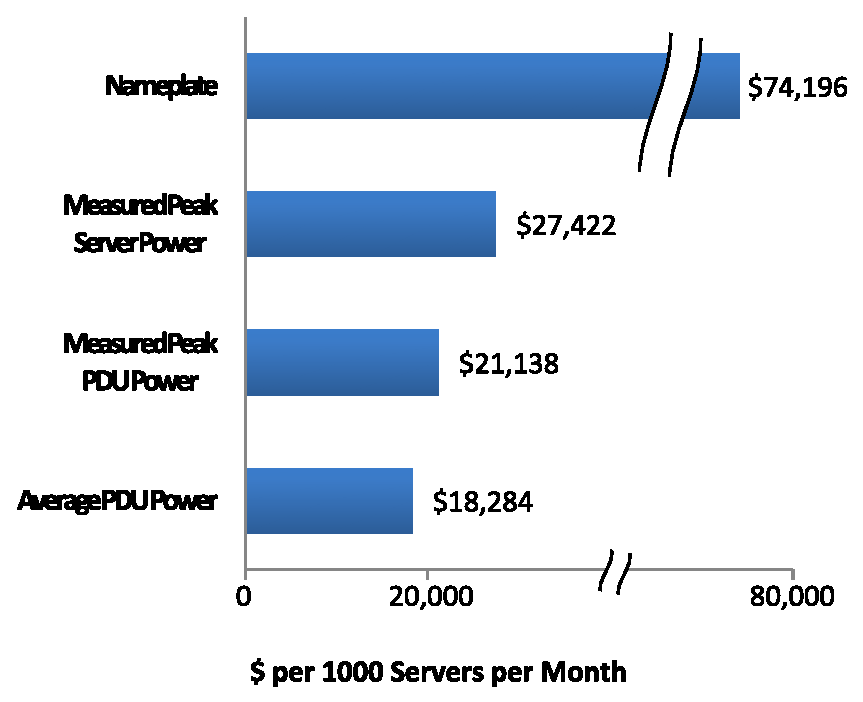
\includegraphics[width = 3.0 in]{Appendices/PowerRouting/figure/intro.eps}
\vspace{-.05 in}
\caption{ \textbf{The cost of over-provisioning.} \textnormal{Amortized monthly cost of power infrastructure for 1000 servers under varying provisioning schemes.}}
\label{figure::intro}
\vspace{-.1 in}
\end{figure}

Although the power demands of individual servers can vary greatly, statistical effects make it unlikely for all servers' demands to peak at the same time \cite{Govindan09,Ranganathan06}. Even in highly-tuned clusters running a single workload, peak utilization is rare, and still falls short of provisioned power capacity \cite{Fan07}.  This observation has lead researchers and operators to propose \emph{over-subscribing} power circuits.  To avoid overloads that might impact availability, such schemes rely on \emph{power capping} mechanisms that enforce power budgets at individual servers \cite{Lefurgy08, Wang08} or over ensembles \cite{Ranganathan06, Wang09}.  The most common power-capping approaches rely on throttling server performance to reduce power draw when budgets would otherwise be exceeded \cite{Lefurgy08,Ranganathan06, Wang08,Wang09}.  

Figure~\ref{figure::intro} illustrates the cost of conservative provisioning and the potential savings that can be gained by over-subscribing the power infrastructure.  The graph shows the amortized monthly capital cost for power infrastructure under varying provisioning schemes.  We calculate costs following the methodology of Hamilton \cite{Hamilton09} assuming high-availability power infrastructure costs \$15 per critical-load Watt \cite{Turner06}, the power infrastructure has a 15-year lifetime, and the cost of financing is 5\% per annum.   We derive the distribution of actual server power draws from 24 hours of data collected from 1000 servers in three production facilities (details in Section \ref{section::methodology}).  Provisioning power infrastructure based on nameplate ratings results in infrastructure costs over triple the facility's actual need.  Hence, operators typically ignore nameplate ratings, instead provisioning infrastructure based on a measured peak power for each class of server hardware.  However, even this provisioning method overestimates actual needs---provisioning based on the observed aggregate peak at any power distribution unit (PDU) reduces costs 23\%. Provisioning for less-than-peak loads can yield further savings at the cost of some performance degradation (e.g., average power demands are only 87\% of peak).  

Power capping makes over-subscribing safe.  However, power budgets must enforce local (PDU) as well as global (uninterruptible power supply, generator and utility feed) power constraints.  Hence, local spikes can lead to sustained performance throttling, even if the data center is lightly utilized and ample power delivery capacity is available elsewhere.  Moreover, in high-availability deployments, the need to maintain reserve capacity on redundant power delivery paths to ensure uninterrupted operation in the event of PDU failure magnifies the impact of utilization spikes---not only does the data center's direct demand rise, but also the potential load from failover.

An ideal power delivery system would balance loads across PDUs to ensure asymmetric demand does not arise.  Unfortunately, since server power demands vary, it is difficult or impossible to balance PDU loads statically, through clever assignment of servers to PDUs.  Such balancing may be achievable dynamically through admission control \cite{Chase01} or virtual machine migration \cite{Clark05}, but implies significant complexity, may hurt performance, and may not be applicable to non-virtualized systems. Instead, in this paper, we explore mechanisms to balance load through the \emph{power delivery infrastructure}, by dynamically connecting servers to PDUs. 

Our approach, \emph{Power Routing}, builds on widely-used techniques for fault-tolerant power delivery, whereby each server can draw power from either of two redundant feeds.  Rather than designating primary and secondary feeds and switching only on failure (or splitting loads evenly across both paths), we instead centrally control the switching of servers to feeds.  The soft-switching capability (already present  for ease of maintenance in many dual-corded power supplies and rack-level transfer switches) acts as the foundation of a power switching network.

In existing facilities, it is common practice for all servers in a rack or row to share the same pair of redundant power feeds, which makes it impossible to use soft-switching to influence local loading.  Our key insight, inspired by the notion of skewed-associative caches \cite{Seznec93} and declustering in disk arrays \cite{Alvarez98}), is to create \emph{shuffled distribution topologies}, where power feed connections are permuted among servers within and across racks. In particular, we seek topologies where servers running the same workload (which are most likely to spike together) connect to distinct pairs of feeds.  Such topologies have two implications.  First, they spread the responsibility to bear a failing PDU's load over a large number of neighbors, reducing the required reserve capacity at each PDU relative to conventional designs.  Second, they create the possibility, through a series of switching actions, to route slack in the power delivery system to a particular server.

Designing such topologies is challenging because similar servers tend to be collocated (e.g., because an organization manages ownership of data center space at the granularity of racks).  Shuffled topologies that route power from particular PDUs over myriad paths require wiring that differs markedly from current practice.  Moreover, assignments of servers to power feeds must not only meet PDU capacity constraints, they must also: (1) ensure that no overloads occur if any PDU fails (such a failure instantly causes all servers to switch to their alternate power feed); and (2) balance power draws across the three phases of each alternating current (AC) power source to avoid voltage and current fluctuations that increase heating, reduce equipment lifetime, and can precipitate failures \cite{Gruzs90}. Even given a shuffled topology, power routing remains challenging: we will show that solving the dynamic assignment of servers to PDUs reduces to the partitioning problem \cite{GareyBook}, and, hence, is NP-complete and infeasible to solve optimally.  In this paper, we address each of these challenges, to contribute:

\begin{packed_itemize}

\item {\bf Lower reserve capacity margins.}   Because more PDUs cooperate to tolerate failures, shuffled topologies reduce per-PDU capacity reserves from 50\% of instantaneous load to a $1/N$ fraction, where $N$ is the number of cooperating PDUs.   
\vspace{4pt}
\item {\bf Power routing.} We develop a linear programming-based heuristic algorithm that assigns each server a power feed and budget to minimize power capping, maintain redundancy against a single PDU fault, and balance power draw across phases.
\vspace{4pt}
\item {\bf Reduced capital expenses.}  Using traces from production systems, we demonstrate that our mechanisms reduce power infrastructure capital costs by 32\% without performance degradation.  With energy-proportional servers, savings reach 47\%.

\end{packed_itemize}

The rest of this paper is organized as follows.  In Section~\ref{section::background}, we provide background on data center power infrastructure and power capping mechanisms.   We describe our mechanisms in Section~\ref{section::powerrouting} and detail \PowerRouting's scheduling algorithm in Section~\ref{section::scheduling}.  We evaluate our techniques on our production data center traces in Section~\ref{section::evaluation}.  Finally, in Section~\ref{section::conclusion}, we conclude. 
. 

 \chapter{Introduction}
 \label{chap:Intro}
 For decades disk has been the primary technology for durable and large-capacity storage.
Although inexpensive and dense, disk provides high performance only for coarse-grained sequential access and suffers enormous slowdowns for random reads and writes.
Recently, several new technologies have emerged as popular or viable storage alternatives.
Flash memory, primarily used for mobile storage, has gained traction as a high-performance enterprise storage solution.
Nonvolatile Random Access Memories (NVRAM), such as phase change memory and spin-transfer torque RAM, have emerged as high performance storage alternatives \cite{BurrKurdi08}.

These technologies offer significant performance improvements over disk, while still providing durability with great storage capacity.
As drop-in replacements for disk, Flash and NVRAM accelerate storage access.
However, the disk interface fails to leverage specific device characteristics.

This thesis investigates how several data-centric workloads interact with future storage technologies, the relevant software and algorithms, and in some instances computer hardware.
Specifically, I consider analytics (commonly Decision Support Systems -- DSS -- popular in ``Big Data") and On-Line Transaction Processing (OLTP), important workloads which generally fit under the broad definition of databases.
Moreover, both workload classes have long been constrained by disk, both in terms of cost and software design complexity.
I match each workload to the emerging storage technology that suits it best and address specific opportunities or deficiencies in the software and hardware systems.

\section{Analytics}
\label{sec:Intro:Analytics}

Analytics relies on disk to provide enormous data capacity.
Typical analytics work-flow involves taking a snapshot of data from an online database and mining this data for complex, yet useful, patterns.
While applications do not rely on disk's durability for recovery (in fact, instances that reasonably fit in main memory have no need for disk), modern analytics data sets reach peta-byte scale \cite{Economist10}, and accessing such large data quickly becomes the dominant bottleneck.
Such capacity is only reasonably achieved by dense disk and Flash memory.

Decades of research have provided modern analytics databases with tools to minimize storage accesses, particularly slow random accesses (e.g., disk-specific indexes, join algorithms to minimize page access and produce large sequential runs).
Whereas these optimizations are still effective for Flash, they fail to fully leverage Flash's ability to read randomly located data quickly, or properly account for Flash's higher throughput reads than writes.
As examples, I consider access paths (various scan types) and join algorithms.
A rule of thumb for scans is that an index should be used when less than 10\% of tuples in a table are returned, otherwise the entire table should be scanned.
The intuition is that locating tuples from an index requires random reads as well as reading additional pages from the index itself.
One would expect this selectivity (10\%) to increase when replacing disk with Flash -- Flash is no longer penalized by random reads, and so prefers access paths which minimize total page accesses.
Similarly, different ad hoc join algorithms (those that do not use indexes: block-nested loops, sort-merge join, and hybrid-hash join) present different storage access patterns and may be variably suited to disk and Flash.

My results, originally presented in ADMS 2010 \cite{PelleyWenisch11} and discussed in Chapter~\ref{chap:FlashOpti}, show that while both previous hypotheses are correct, their significance is negligible.
Optimal access path (index vs table scan) only changes between disk and Flash for a small range of query selectivities, and queries within that range see only a small performance improvement.
Additionally, join algorithm choice makes little difference, as optimized join algorithms exhibit nearly balanced read and write capacity in large sequential runs -- join algorithms optimized for disk are already optimized for Flash.
I conclude that the page-oriented nature of Flash limits further analytics-Flash optimization.
Next, I turn to NVRAM's possible database uses.

\section{Transaction Processing}
\label{sec:Intro:OLTP}

While NVRAM's promising data capacity would additionally benefit analytics, the resulting software design would closely resemble DRAM-based analytics, a largely solved problem; in general analytics does not take advantage of NVRAM's persistence.
However, NVRAM can also be used to provide failure recovery for durable transactions.
Databases have been designed for decades to provide high-throughput transaction processing with disk.
Write Ahead Logging (WAL) techniques, such as ARIES \cite{MohanHaderle92}, transform random writes into sequential writes and minimize transactions' dependences on disk accesses.
With sufficient IOPS and read-buffering, databases can be made compute-bound and recover near-instantly.
NVRAMs provide this massive storage throughput, which I expect will provide high transaction performance and low recovery latency to the masses.

Whereas ARIES was necessary for disk, it presents only unnecessary software overheads to NVRAM.
I show that removing ARIES improves transaction throughput by alleviating software bottlenecks inherent in centralized logging.
Instead, NVRAM allows data to be updated in-place, enforcing data persistence immediately and providing correct recovery via transaction-local undo logs.

NVRAMs, however, are not without their limitations.
Se\-veral candidate NVRAM technologies exhibit larger read latency and significantly larger write latency compared to DRAM \cite{BurrKurdi08}.
Additionally, whereas DRAM writes benefit from caching and typically are not on applications' critical paths, NVRAM writes must become persistent in a constrained order to ensure correct recovery.
I consider an NVRAM access model where correct ordering of persistent writes is enforced via \emph{persist barriers}, which stall until preceding NVRAM writes complete; such persist barriers introduce substantial delays when NVRAM writes are slow.

To address these challenges I investigate accelerating NVRAM reads with various cache architectures and capacities, and avoid persist barrier delays by introducing a new recovery mechanism, \GroupCommit.
NVRAM designs are discussed in Chapter~\ref{chap:OLTP_design}.
I show that fast, memory-bus-connected NVRAM needs no additional caching (on-chip caches suffice) and that updating data in-place is a simple and viable recovery strategy.
However, long latency interconnects (e.g., Non-Uniform Memory Architectures -- NUMA, PCIe-attached NVRAM, or distributed storage) require additional caching and benefit from \GroupCommit.
Chapter~\ref{chap:OLTP_eval} presents an evaluation of NVRAM OLTP.
This work is currently under review at VLDB.

\section{Persistent Memory Consistency}
\label{sec:Intro:PMC}

Finally, I propose the final project of my thesis.
The previous work looks at how OLTP recovery mechanisms should be designed, considering only the average delay incurred by persist barriers.
I intend to investigate specific programming models to provide persist barriers, considering their probable performance and ease of programming.
I extend the concept of memory consistency with persistence to introduce \emph{Persistent Memory Consistency} (PMC).

Similar to volatile memory consistency, persistent consistency presents trade offs between hardware complexity, performance, and ease of programming.
I explore existing solutions, describe why they fall short, and place them into a more precisely defined taxonomy of persistent consistency.
Further, I introduce examples of relaxed consistency and how they improve performance in Chapter~\ref{chap:PMC}.
Finally, I highlight new optimizations for persist barriers and persistent consistency, providing example persistent data structures in Chapter~\ref{chap:PMC_patterns}.
Future work will include performance evaluations, new consistency models, new data structures, and potential optimizations.

\section{Additional Work}
\label{sec:Intro:Additional}
The primary themes of this thesis include performance, cost efficiency, and reliability.
While I focus on storage architectures, I have published additional work regarding the cost and reliability of data center infrastructure.
Appendix~\ref{app:WEED} contains ``Understanding and Abstracting Total Data Center Power," \cite{PelleyMeisner09} published at WEED 2009.
This work presents power/energy models for all aspects of the data center, including power distribution, battery backups, cooling infrastructure, and IT equipment.
Appendix~\ref{app:PowerRouting} contains ``PowerRouting: Dynamic Power Provisioning for the Data Center," \cite{PelleyMeisner10} published at ASPLOS 2010.
PowerRouting distributes power infrastructure throughout the data center to minimize installed power infrastructure capacity while maintaining reliability, minimizing data center cost.
The key insight is that data centers typically over-provision infrastructure, resulting in under-utilized (and often unnecessary) equipment.
PowerRouting leverages compute-specific knowledge of the IT workload to more effectively utilize power infrastructure.
Both of these works are included without modification.

My focus shifted away from data center infrastructure as I realized it was primarily an efficiency, not computing, problem.
That is, industry is effectively solving power and infrastructure problems by providing more efficient, cost-effective components (more efficient servers, efficient cooling, high density density).
As these components improve, the opportunity to use compute-specific knowledge to make an impact diminishes.
Instead, I turned to emerging storage technologies.

\section{Summary}
\label{sec:Intro:Summary}
This proposal is formatted according to thesis guidelines for the University of Michigan.
Where possible, I intend to use portions of the proposal in my final thesis.
Chapter~\ref{chap:Background} contains background information on storage technologies and database optimizations.
This background forms the foundation of the work that follows.
Chapter~\ref{chap:FlashOpti} considers taking advantage of Flash's fast random reads to accelerate database analytics.
I consider this work complete and do not propose any extension.
In Chapter~\ref{chap:OLTP_design} I describe potential software designs for OLTP using NVRAM and a methodology to evaluate NVRAM (devices that do not currently exist) on modern hardware.
I propose additional work to extend and complete this project in Sections~\ref{sec:OLTP_design:GroupCommit:Proposed} and~\ref{sec::OLTP_design:GroupCommit:Proposed}.
Chapter~\ref{chap:OLTP_eval} uses my methodology to evaluate several aspects of OLTP running on NVRAM.
Again, I propose additional evaluations in Section~\ref{sec:OLTP_eval:Proposed}.
Chapters~\ref{chap:PMC} and~\ref{chap:PMC_patterns} describe in-progress work on persistent memory consistency, persistent data structures, and their performance.
The ideas contained in those chapters are not entirely mature and I welcome feedback.


 \chapter{Background}
 \label{chap:Background}
 This chapter provides details necessary to understand the investigations and experiments in this thesis.
I focus on storage technologies, database analytics optimization, database transaction processing optimizations, and memory consistency models.
The purpose of discussing database optimizations is to understand the complications that arise when using disk, and how resulting mechanisms interact with new storage technologies.
Additionally, memory consistency forms the foundation for memory persistency.

\section{Storage Technologies}
\label{sec:Background:Storage}

Many technologies provide storage persistent storage, including disk, Flash, and upcoming NVRAM.
For each, I outline the operating principles and important technological trends.

\begin{table}
  \centering
  \begin{tabular}{ l l l }
  %\begin{tabular}{r@{\hspace{12pt}}c@{\hspace{12pt}}c@{\hspace{12pt}}}
  \toprule
   & Disk & Flash \\
   \midrule
   Model & WD VelociRaptor 10Krpm & OCZ RevoDrive \\
   Capacity & 300gb & 120gb \\
   Price & \$164 & \$300 \\
   Random Read & 10ms & 90$\muup$s \\
   Seq. Read & 120mb/s & 190mb/s \\
  \bottomrule
  \end{tabular}

  \caption{Disk Characteristics}
  \label{table::DiskCharacteristics}
\end{table}


\subsection{Disk}
\label{sec:Background:Storage:Disk}
Disk has been the primary durable and high capacity storage technology for decades.
Disk functions by storing data on spinning magnetic platters.
Accessing data requires moving the \emph{hard disk head} onto the proper \emph{track}.
Once the head settles, it may read or write data as the platter rotates and the correct sector within the track reaches the head.
Disk capacity increases with the areal size and number of platters, as well as areal density (placing more sectors and tracks within the same area).
Because capacity has scaled so well (and continues to), disk remains the lowest cost technology for large datasets and persistent storage.

While popular and inexpensive, disk suffers relatively slow access and undesirable access behavior \cite{RuemmlerWilkes94}.
Rotational speed limits the rate that data transfers to or from the disk.
Further, random reads and writes must first seek to the proper track and then wait until the correct sector reaches the head, a process which takes several ms.
Table~\ref{table:DiskCharacteristics} lists the measured performance characteristics of an enterprise disk (2011).
This disk achieves nearly 120 MB/s sequential transfers, but random reads take an average of 10ms (only 50 KB/s for 512-byte sectors).
As a result, there is a large history of optimization for disk-resident storage, as I discuss in Section~\ref{sec:Background:Recovery}.

\subsection{Flash Memory}
\label{sec:Background:Storage:Flash}
Driven by the popularity of mobile devices, Flash memory has quickly improved in both storage density and cost to the point where it has become a viable alternative for durable storage in enterprise systems.
Unlike conventional rotating hard disks, which store data using magnetic materials, Flash stores charge on a floating-gate transistor forming a memory cell.
These transistors are arranged in arrays resembling NAND logic gates, after which the ``NAND Flash'' technology is named.
This layout gives NAND Flash a high storage density relative to other memory technologies.
Though dense, the layout allows only coarse-grained access and sacrifices read latency---an entire array (a.k.a. page, typically 2KB to 4KB) must be read in a single operation---making NAND Flash more appropriate for block-oriented IO than as a direct replacement for RAM.  

One of the difficulties of Flash devices is that a cell can be more easily programmed (by adding electrons to the floating gate) than erased (removing these electrons).  
Erase operations require both greater energy and latency, and typically can be applied only at coarse granularity (e.g., over blocks of 128KB to 512KB).
Moreover, repeated erase operations cause the Flash cell to wear out over time, limiting cell lifetime (e.g., to $10^5$ to $10^6$ writes \cite{Roberts2009}).  
Recent Flash devices further increase storage density by using several distinct charge values to represent multiple bits in a single cell at the cost of slower accesses and even shorter lifetimes.

A Flash-based SSD wraps an array of underlying Flash memory chips with a controller that manages capacity allocation, mapping, and wear leveling across the individual Flash devices.  
The controller mimics the interface of a conventional (e.g., SATA) hard drive, allowing Flash SSDs to be drop-in replacements for conventional disks.
      
As previously noted, Flash SSDs provide substantially better performance than disks, particularly for random reads, but at higher cost \cite{BoboilaDesoyers11}.
Table \ref{table:DiskCharacteristics} lists specifications of a typical Flash SSD as compared to a 10,000 RPM hard drive (2011).
Though neither of these devices are the highest-performing available today, they are representative of the mid-range of their respective markets.
The latency for a random read is over 100\texttimes~better on the SSD than on the disk, while the sequential read bandwidth is 1.6\texttimes~better. 
Unlike disks, where each random read incurs mechanical delays (disk head seek and rotational delays), on SSDs, a random read is nearly as fast as a sequential read.  

\subsection{NVRAM}
\label{sec:Background:Storage:NVRAM}

Nonvolatile memories will soon be commonplace.
Technology trends suggest that DRAM and Flash memory may cease to scale, requiring new dense memory technologies \cite{LeeIpek09}.

\textbf{Memory technology characteristics.}
Numerous technologies offer durable byte-addressable access.
Examples include phase change memory (PCM), where a chalcogenide glass is heated to produce varying electrical conductivities, and spin-transfer torque memory (STT-RAM), a magnetic memory that stores state in electron spin \cite{BurrKurdi08}.
Storage capacity increases by storing more than two states per cell in Multi-level Cells (MLC) (e.g., four distinct resistivity levels provide storage of 2 bits per cell).

While it remains unclear which of these technologies will eventually gain traction, many share common characteristics.
In particular, NVRAMs will likely provide somewhat higher access latency relative to DRAM.
Furthermore, several technologies are expected to have asymmetric read-write latencies, where writing to the device may take several microseconds \cite{QureshiSrinivasan09}.
Write latency worsens with MLC, where slow, iterative writes are necessary to reliably write to cells.

Similarly to Flash, resistive NVRAM technologies suffer from limited write endurance; cells may be written reliably a limited number of times.
While write endurance is an important consideration, proposed hardware mechanisms (e.g., Start-Gap \cite{QureshiKaridis09}) are effective in distributing writes across cells, mitigating write endurance concerns.

\textbf{NVRAM storage architectures.}
Future database systems may incorporate NVRAM in a variety of ways.
At one extreme, NVRAM can be deployed as a disk or Flash SSD replacement.
While safe, cost-effective, and backwards compatible, the traditional disk interface imposes overheads.
Prior work demonstrates that file system and disk controller latencies dominate NVRAM access times \cite{CaulfieldDe10}.
Furthermore, block access negates advantages of fine-grained access.

Recent research proposes alternative interfaces for NVRAM.
Caulfield \emph{et al.} propose Moneta and Moneta Direct, a PCIe attached PCM device \cite{CaulfieldMollov12}.
Unlike disk, Moneta Direct bypasses expensive system software and disk controller hardware to minimize access latency while still providing traditional file system semantics.
However, Moneta retains a block interface.
Condit \emph{et al.} suggest that NVRAM connect directly to the memory bus, with additional hardware and software mechanisms providing file system access and consistency \cite{ConditNightingale09}.
I later adopt the same atomic eight-byte persistent write, enabling small, safe writes even in the face of failure.
NVRAM will eventually connect via a memory interface, but it is unclear how storage technologies will evolve or what their exact performance characteristics will be.
Instead of assuming specific NVRAM technologies and interconnects, I measure the affect that NVRAM performance (both latency and bandwidth) has on workload throughput.

\section{Analytics Optimization}
\label{sec:Background:Analytics}

Large scale data processing requires efficient use of storage devices.
Relational data is stored in tables (relations).
Tables are a collection of rows (tuples), each row containing values for the different columns (attributes) defined on the table.
I discuss two important operations common to the relational model that are expected to be affected by Flash's performance characteristics: scans and joins.

\subsection{Scans}
\label{sec:Background:Scans}

Each data access requires the query optimizer to choose access paths to each table. 
The goal is to select all relevant rows from the table while retrieving the fewest storage pages, frequently with the use of indexes.
Work on access path selection dates back to the late 1970s \cite{Selinger1979}.

There are two classic scan operators implemented by nearly all commercial DBMS systems: relation scan and index scan.
An index is a database data structure that maps column values to rows within a table, supporting fast look-ups by that column.
Indexes may be ordered (as in an in-memory balanced tree or disk-resident B-Tree) to efficiently retrieve all rows satisfying a range query (e.g., an ordered index on ``last name" would accelerate a query asking for all people whose last name is between ``Pelley" and ``Wenisch").
Additionally, indexes may be clustered (the primary table is stored in sorted/hashed order and supports searching) or non-clustered (the index is separate from the primary store and contains references to rows).
A table can only be physically ordered according to one key, limiting the use of clustered indexes.
Database indexes are themselves stored on disk.
Many types of indexes exist, but all provide a more direct way to filter specific data than scanning an entire data set.

When no indexes are available, the only choice is to perform a \emph{relation scan}, where all data pages in the table are read from disk and scanned tuple-by-tuple to select tuples that satisfy the query.
When a relevant index is available, the DBMS may instead choose to perform an \emph{index scan}, where the execution engine traverses the relevant portion of the index and fetches only pages containing selected tuples as needed.
For clustered indexes (i.e., the row itself exists within the index, and all rows are sorted according to the index key), an index scan is nearly always the preferred access path, regardless of the underlying storage device.  
For non-clustered indexes, whether the optimizer should choose a relation scan or index scan depends on the selectivity of the query (expected number of rows that satisfy the query); relation scans have roughly constant cost regardless of selectivity (cost depends on table size), whereas index scan costs grow approximately linearly with selectivity.
When selectivity is low, the index scan provides greater performance because it minimizes the total amount of data that must be transferred from disk.
However, as selectivity increases, the fixed-cost (and simpler) relation scan becomes the faster option.  
Though the relation scan reads the entire table, it can do so using sequential rather than random IO, leveraging the better sequential IO performance of rotating hard disks.
A classic rule of thumb for access path selection is to choose a relation scan once selectivity exceeds ten percent \cite{RamakrishnanAndGehrke}.

Recent databases implement a third, hybrid scan operator, which I call \emph{rowid-sort scan}.
In this scan operator, the unclustered index is scanned to identify relevant tuples.
However, rather than immediately fetching the underlying data pages, the rowid (a unique identifier that signifies the row's page and offset within that page) of each tuple is stored in a temporary table, which is then sorted at the end of the index scan.
Then, the pages identified in the temporary table are fetched in order, and relevant tuples are returned from the page.
The rowid-sort scan has the advantage that each data page will be fetched from disk only once, even if multiple relevant tuples are located on the page. 
Rowid-sort scan is provided by IBM's DB2, although they may refer to it by a different name.
Other databases use different terminology or algorithms to ensure that each heap page is fetched exactly once (for example, PostgreSQL uses a bitmap index, sorting the list of pages with tuples that satisfy the query \cite{PostgresLossyBitMap}).
Rowid-sort scan is the optimal access path for intermediate selectivities.
Section~\ref{sec:FlashOpti:Scans} investigates choosing an optimal access path depending on whether data resides on disk or Flash.

\subsection{Joins}
\label{sec:Background:Joins}

One of the most important aspects of query optimization is choosing appropriate join algorithms.
The development of join algorithms and optimization strategies dates back over 30 years \cite{Selinger1979,Shapiro1986}. 
Most commercial DBMS systems implement variants of at least three join algorithms: nested-loop join, sort-merge join, and hybrid hash join.
At a high level, the nested-loop join iterates over the inner relation for each tuple of the outer relation; the sort-merge join sorts both relations and then performs concurrent scans of the sorted results; and the hybrid hash join forms in-memory hash tables of partitions of the inner relation and then probes these with tuples from the outer relation.

The relative performance of these algorithms depends on a complex interplay of memory capacity, relation sizes, and the relative costs of random and sequential IOs.  
One example performance model that captures this interplay was proposed by Haas and co-authors \cite{DBLP:journals/vldb/HaasCLS97}.
Their model estimates the number of disk seeks and the size of each data transfer and weights each by a cost based on assumed characteristics of the IO device.
The model further identifies the optimal buffering strategy for the various phases of each join algorithm.
Seek and random/sequential transfer times are central parameters of this model, suggesting that new technologies require new device-specific query optimization.

As accessing large amounts of data on disk can limit system throughput, it is imperative that the query optimizer choose the best query plan.
Typical query optimizers use data statistics to approximate query selectivity and cardinality as well as physically-based models to estimate the runtime of candidate query plans.
Sections~\ref{sec:FlashOpti:Scans} and~\ref{sec:FlashOpti:Joins} will investigate when the query plan changes between disk and Flash, and what performance is lost when the incorrect decision is made (assuming disk but actually using Flash).

\section{Durable and Recoverable Transactions}
\label{sec:Background:Recovery}

Many database applications require transaction semantics commonly described as ACID (Atomic, Consistent, Isolated, Durable) \cite{Gray81}.
While the first three are primarily impacted by the database's concurrency control mechanisms within main memory, transaction durability and database recovery interacts with persistent storage.
The goal of recovery management is to ensure that during normal transaction processing no transaction reports that it has committed and is later lost after a system failure, and that any transaction that fails to commit before a failure is completely removed (i.e., no partial updates remain).
Additionally, recovery should occur as quickly as possible and allow efficient forward processing.
Several schemes provide correct, high performance recovery for disk.
I describe ARIES \cite{MohanHaderle92}, a popular Write Ahead Logging (WAL) system that provides atomic durable transactions.

\textbf{ARIES.}
ARIES uses a two-level store (disk and volatile buffer cache) alongside a centralized log.
The buffer cache is necessary to accelerate reads and defer writes to the disk.
Transaction writes coalesce in the buffer cache while being durably recorded in the log as ordered entries that describe page updates and actions, transforming random writes into sequential writes.

The log improves disk write performance while simultaneously providing data recovery after failure.
Transaction updates produce both redo and undo entries.
Redo logs record actions performed on heap pages so that they can be replayed if data has not yet written to disk in-place.
Undo logs provide roll back operations necessary to remove aborted and uncommitted transaction updates during recovery.
The database occasionally places a checkpoint in the log, marking the oldest update within the database still volatile in the buffer cache (and therefore where recovery must begin).
Recovery replays the redo log from the most recent checkpoint to the log's end, reproducing the state at failure in the buffer cache; ARIES ``replays history," recovering the failed database.
Afterwards, incomplete transactions are removed using the appropriate undo log entries.

While a centralized log orders all database updates, the software additionally enforces that log entries are durable before heap pages write back for each operation.
Transactions commit by generating a commit log entry, which must necessarily become durable after the transaction's other log entries (since the log writes to disk in order).
This process guarantees that no transaction commits, or page writes back to disk, without a durable history of its modifications in the log.

Though complex, ARIES improves database performance with disk.
First, log writes appear as sequential accesses to disk, maximizing device throughput.
Additionally, aside from reads resulting from buffer cache misses, each transaction depends on device access only at commit to flush log entries.
All disk writes to the heap may be done at a later time, off of transactions' critical paths.
In this way ARIES is designed from the ground up to minimize the effect of large disk access latencies.

\section{Memory consistency models}
\label{sec:Background:MemoryConsistency}

This section provides a background on memory consistency models, outlining three models: Sequential Consistency (SC), Total Store Order (TSO), Relaxed Memory Order (RMO), and Release Consistency (RC).
Much of this discussion assumes that caches are completely coherent---that is, any two accesses to a cache line (by any core/thread) have a total order.
Release Consistency may guarantee this property only for properly annotated programs.
Other systems enforce cache coherence in hardware without annotation.

Consistency models define the order of loads and stores observed by threads.
While every thread observes its own execution in program order, it may appear that other threads execute out of order.
Processors (and compilers) are generally free to reorder instructions to accelerate performance so long as they produce equivalent results assuming no shared memory accesses (single thread execution).
Loads and stores that are independent from a single-threaded point of view may in fact interact with other threads.
Reordering these memory accesses often results in unintended program behavior.

Two popular solutions to this problem are to (1) force all threads to observe the loads and stores of other threads in a single globally defined order (SC) or (2) relax this guarantee, introducing memory barriers that allow the programmer to enforce a certain order when necessary (i.e., relax consistency).
While relaxing consistency may provide higher performance, it places a greater burden on programmers to be aware of instruction reordering and correctly use memory barriers.

The consistency model provides the programming abstraction and guarantees on observed memory orders that the programmer can expect.
Implementations may momentarily violate the consistency model so long as no program is able to observe the violation.
For example, implementations are free to \emph{speculate}, executing with relaxed consistency, and later determine whether consistency has been violated.
When consistency is violated the implementation must rollback and re-execute memory instructions, providing the illusion that threads execute with strict consistency.

\textbf{Sequential Consistency.}
Sequential Consistency \cite{Lamport79} provides the most intuitive programming model, yet necessarily the worst performance (although modern techniques use speculation to improve performance).
All loads and stores appear in a globally consistent order that is an interleaving of program order of all threads.
A popular view of SC is that memory switches between the various processors; only a single processor accesses memory at any single time.
Additionally, many architectures define atomic Read-Modify-Write operations (RMW; e.g., compare-and-swap, atomic add).
The programmer need not consider memory instructions reordering; barriers are unnecessary (compiler barriers must still be used).

\textbf{Total Store Order.}
Total Store Order \cite{SPARCv9} provides greater performance than SC at the cost of requiring the programmer to insert memory barriers.
Most memory operations in each thread are still observed to occur in program order: (1) stores may not reorder with other stores, (2) loads may not reorder with other loads, and (3) a store that occurs after a load may not reorder and appear to occur before that load.
These rules guarantee that all stores occur in a globally consistent sequential order.
However, loads that occur after a store in program order may reorder and bypass the store, appearing to occur before the store from the perspective of other processors.
The justification for doing this is that stores are typically not on the application's critical path -- they simply write into the cache and do not result in delays.
Loads, on the other hand, may stall due to cache misses.
Executing loads as soon as possible minimizes delays.

The programmer is responsible for recognizing any code where allowing a load to bypass a store causes an incorrect result.
A barrier is provided by the architecture for such cases to force all loads to delay until the store appears to other threads (or re-execute those loads if some other thread issues conflicting stores).
RMW instructions act as as barrier, preventing memory operations from reordering.
As concurrent programming commonly uses RMW operations, explicit memory barriers are rarely required in practice.

\textbf{Relaxed Memory Order.}
Relaxed Memory Order \cite{SPARCv9} further relaxes consistency, allowing stores and loads to reorder around each other.
To enforce the intended behavior the programmer must use memory barriers to constrain memory operation order.
RMO barriers constrain (1) loads from reordering with other loads, (2) stores from reordering with other stores, (3) loads from bypassing stores, and (4) stores from bypassing loads.
Any of these constraints may be enforced at a memory barrier.
RMO requires frequent barriers for correct thread communication.

\textbf{Release Consistency.}
Release Consistency \cite{GharachorlooLenoski90} provides a relaxed consistency model with two barriers -- acquire and release.
In the absence of barriers threads may observe memory operations in any order and may read stale data (some other processor wrote to an address but an older value is loaded).
Before reading shared memory an \emph{acquire} barrier must be used to label the access as an acquire event.
Similarly, after writing to shared memory a \emph{release} barrier is used; acquire and release used as a pair ensure that written data is observed by other processors.
Additionally, acquire and release barriers prevent memory operations from reordering (for example, to ensure that operations in a critical section occur only after the lock is acquired and before the lock is released).
RMW operations implicitly contain both acquire and release barriers.

Release Consistency improves performance by (1) relaxing all consistency guarantees for single threaded code, (2) providing precise memory barriers, and (3) enforcing cache coherence only at barriers.
Acquire and release barriers order only certain types of accesses, leaving other accesses unconstrained.
However, release consistency requires the programmer to be aware of and understand these persist barriers.

A similar trade-off exists for enforcing data persistence---Persistence constraints are relaxed so that persist order may not match program order and may not appear as a valid interleaving of all persists.
Removing NVRAM write constraints improves performance while still providing mechanisms to enforce expected behavior.
The interaction between persistence, performance, and programmability is explored in Chapter~\ref{chap:Persistency}.

\section{Conclusion}
\label{sec:Background:Conclusion}

This chapter provides a brief history and outline of storage devices, database technologies, and memory consistency interfaces.
The remainder of thesis builds on these ideas to explore how best to use NVRAM in future memory systems.


 \chapter{SSD-aware Query Optimization}
 \label{chap:FlashOpti}
 This chapter attempts to determine if database query optimizers must be SSD-aware.
The work was originally published in the Second International Workshop on Accelerating Data Management Systems Using Modern Processor and Storage Architectures (AMDS 2011), collocated with VLDB \fixme{cite}.
I worked on this project with my advisor, Thomas F. Wenisch, and assistant professor Kristen LeFevre.
Working under their advisement, I was the sole graduate student and technical contributor (database and programming effort).
Refer to Sections~\ref{sec:Background:Storage} and~\ref{sec:Background:Analytics} for necessary background on this topic.
While the project ended in a negative result, it was instrumental developing my understanding of databases and storage management.
After completing this work I moved from considering flash to emerging NVRAM technologies; I propose no future work or extensions to this chapter.

\section{Introduction}
\label{sec:FlashOpti:Intro}

For decades, database management systems (DBMSs) have used rotating magnetic disks to provide durable storage.
Though inexpensive, disks are slow, particularly for non-sequential access patterns due to high seek latencies.
With the rapid improvements in storage density and drop in price of Flash-based Solid State Disks (SSDs), DBMS administrators are beginning to supplant conventional rotating disks with SSDs for performance-critical data in myriad DBMS applications.
Though SSDs are several factors more expensive than conventional disks (in terms of \$ per GB), they provide modest (2\texttimes) improvements in sequential IO and drastic (over 100\texttimes) improvements for random IO, closing the gap between these access patterns.

Many components of modern DBMSs have been designed to work around the adverse performance characteristics of disks (e.g., page-based buffer pool management, B-tree indexes, advanced join algorithms, query optimization to avoid non-sequential IO, prefetching, and aggressive IO request reordering).  
As SSDs present substantially different performance trade-offs, over the past few years researchers have begun to examine how SSDs are best deployed for a variety of storage applications \cite{Bouganim09uflip:understanding, Chen2009}, including DBMSs \cite{Lee2008, Yin2009, Li2009, Baumann2010, Tsirogiannis2009}.  
A common theme among these studies is to leverage the better random IO performance of SSDs through radical redesigns of index structures \cite{Yin2009, Li2009} and data layouts \cite{Baumann2010, Tsirogiannis2009}. 
However, even within the confines of conventional storage management and indexing schemes in commercial DBMSs, there may be substantial opportunity to improve query optimization by making it SSD-aware.

In this chapter, I examine the implications that moving a database from disk to Flash SSDs will have for query optimization in conventional commercial DBMSs.
I focus on optimization of read-only queries (e.g., as are common in analytics decision support workloads) as these operations are less sensitive to the SSD adoption barriers identified in prior work, such as poor SSD write/erase performance \cite{Chen2009} and write endurance \cite{Roberts2009}.
Conventional query optimizers assume a storage cost model where sequential IOs are far less costly than random IOs, and select access paths and join algorithms based on this assumption.
The recent literature \cite{Baumann2010} suggests that on SSDs, optimizers should instead favor access paths using non-clustered indexes more frequently; SSDs will favor retrieving more rows via an index if it reduces the number of pages accessed, even if it increases random IO accesses.
Furthermore, as SSDs change the relative costs of computation, sequential, and random IO, the relative performance of alternative join algorithms should be re-examined, and optimizer cost models updated.

My original intent was to leverage this idea to 1) improve query optimization by making device-specific decisions, and 2) accelerate database analytics and reduce operating costs by intelligently placing data on different devices.
While flash is faster than disk, it is generally more expensive per equal capacity.
It makes sense to place small amounts of frequently accessed data on flash, and the rest on disk.
Furthermore some data ``prefers" to live on flash as it is accessed in ways that flash can take advantage of (e.g., queries typically access this data in selectivities or join types that prefer flash).

Despite this intuition, my empirical investigation using a commercial DBMS finds \emph{it is not necessary to make any adjustments to the query optimizer when moving data from disk to Flash}---an SSD-oblivious optimizer generally makes effective choices.
I demonstrate this result, and explore why it is the case, in two steps.

First, I analyze the performance of scan operators.  
Classic rules of thumb suggest that non-clustered index scans are preferable at low selectivity (e.g., below 10\%), whereas a relation scan is faster at high selectivity, because it can leverage sequential IOs.
Therefore, the optimizer should prefer index scans at much higher selectivities on SSDs.  
I demonstrate analytically and empirically that this intuition is false---the range of selectivities for which an index scan operation can benefit from SSDs' fast random reads is so narrow that it is inconsequential in practice.

Second, I measure the relative performance of hybrid hash and sort-merge joins on disk and Flash.
My results indicate that the performance variation between the join algorithms is typically smaller (and often negligible) on Flash, and is dwarfed by the 5\texttimes~to 6\texttimes~performance boost of shifting data from disk to SSD.
 I conclude that because commercial DBMSs have been so heavily optimized to hide the long access latencies of disks (e.g., through sophisticated prefetching and buffering), they are largely insensitive to the latency improvements available on SSDs.
Overall, the small and inconsistent performance gains available by making query optimizers SSD-aware are not worth the effort.

\section{Methodology}
\label{sec:FlashOpti:Methodology}
The objective of this empirical study is to contrast the performance of alternative scan and join algorithms for the same queries to discover whether the optimal choice of access path or join algorithm differs between SSDs and conventional disks.
For either storage device, the optimal access path depends on the selectivity of the selection predicate(s).
The optimal join algorithm depends on several factors: the sizes of the inner and outer relations, the selectivity and projectivity of the query, the availability of indexes, and the available memory capacity.
The goal is to determine whether the regions of the parameter space where one algorithm should be preferred over another differ substantially between SSD and disk because of the much better random read performance of the SSD.
In other words, I am trying to discover, empirically, cases where an access path or join algorithm that is an appropriate choice for disk results in substantially sub-optimal performance on an SSD, suggesting that the optimizer must be SSD-aware.

I carry out this empirical investigation using IBM DB2 Enterprise Server Edition version 9.7.
Experiments use the Wisconsin Benchmark schema \cite{Bitton83benchmarkingdatabase} to provide a simple, well-documented dataset on which to perform scans and joins.
Though this benchmark does not represent a particular real-world application, modeling a full application is not our intent.
Rather, the Wisconsin Benchmark's uniformly distributed fields allows us to control precisely the selectivity of each query.
Whereas real world queries are more complicated than the simple scans and joins we study, these simple microbenchmarks reveal the underlying differences between the storage devices and scan/join algorithms most clearly.
Alternative ``real world" benchmarks (namely TPC-H \fixme{cite}) complicate matters, making it difficult to discern why different query plans prefer disk or SSD.
I aggregate results of all queries to avoid materializing output tables as I am primarily interested in isolating other database operations; typically all results must be aggregated regardless of device, so we remove this step to provide a better comparison.
I run queries on a Pentium Core Duo with 2GB main memory, a 7200 RPM root disk drive, and the conventional and SSD database disks described in Table \ref{table::DiskCharacteristics}.
Both the hard disk and SSD were new at the beginning of the experiments.
While other work has shown that SSD performance may degrade over the lifetime of the device I did not observe any change in performance.

Note that I am not concerned with the optimization decisions that DB2 presently makes for either disk or SSD; rather, I am seeking to determine the ground truth of which algorithm a correct optimizer should prefer for each storage device. 
Originally, I achieved this by varying input parameters to the query optimizer, namely the disk seek latency and sequential access throughput.
Ultimately I discovered that query plan can be established directly by the user, and used DB2's optimization profiles to explicitly set the query plan for each query.


 \chapter{Architecting Recovery Management for NVRAM}
 \label{chap:OLTP_design}
 The following two chapters consider the impact of using emerging NVRAM technologies for durable transaction processing.
Refer to Section~\ref{sec:Background:Storage:NVRAM} for an overview of storage technologies and Section~\ref{sec:Background:Recovery} for a description of ARIES, a popular recovery mechanism for disk.
Work relating to the next two chapters is currently under review at VLDB.
I completed this work under the guidance of my advisor, Thomas F. Wenisch, and collaborators at Oracle, Brian T. Gold and Bill Bridge.
I was the sole graduate student and technical contributer (programming and running experiments) for the project, although my co-authors heavily contributed to developing the following ideas.
I would especially like the thank Brian and Bill for bringing industry's point of view and ``real world" examples to this collaboration.

This chapter outlines the problems with existing disk recovery management, the potential pitfalls of using NVRAM for persistent applications, a methodology for evaluating NVRAM devices that are not yet available, and a description of several candidate software designs for NVRAM recovery management, to be evaluated in the next chapter.
I consider this chapter largely complete with two exceptions.
First, I have validated my timing model and intend to include results in the final thesis \ref{sec:OLTP_design:Methodology:Proposed}.
Second, my implementation of \GroupCommit is more complex than a 12 page journal paper allows room to describe.
I intend to include a detailed description in Section~\ref{sec::OLTP_design:GroupCommit:Proposed}.

\section{Introduction}
\label{sec:OLTP_design:Intro}

Emerging nonvolatile memory technologies (NVRAM) offer an alternative to disk that is persistent, provides read latency similar to DRAM, and is byte-addressable \cite{BurrKurdi08}.
Such NVRAMs could revolutionize online transaction processing (OLTP), which today must employ sophisticated optimizations with substantial software overheads to overcome the long latency and poor random access performance of disk.
Nevertheless, many candidate NVRAM technologies exhibit their own limitations, such as greater-than-DRAM latency, particularly for writes \cite{LeeIpek09}.

These NVRAM technologies stand to revolutionize Online Transaction Processing (OLTP), where consistency and durability are paramount, but applications demand high throughput and low latency.
Prior work has already demonstrated the potential of these technologies to enhance file systems \cite{GreenanMiller06, ConditNightingale09} and persistent data structures \cite{VenkataramanTolia11}, but has not considered OLTP. 
Today, OLTP systems are designed from the ground up to circumvent disk's performance limitations.
For example, many popular database systems use Write-Ahead Logging (WAL; e.g., ARIES \cite{MohanHaderle92}) to avoid expensive random disk writes by instead writing to a sequential log.  
Although effective at hiding write latency, WAL entails substantial software overheads.

NVRAM offers an opportunity to simultaneously improve database forward-processing throughput and recovery latency by rethinking mechanisms that were designed to address the limitations of disk.
Figure~\ref{fig::Recovery} demonstrates this potential, displaying recovery time and transaction throughput for the TPCB workload running on the Shore-MT storage manager \cite{JohnsonPandis09} for hypothetical NVRAM devices (see Section~\ref{sec:OLTP_design:Methodology} for a description of the methodology).

\begin{figure}
  \centering
  \includegraphics[width=.7\linewidth]{OLTP_design/TPCB_Recovery.pdf}
  \caption{\textbf{TPCB recovery latency vs throughput.} Increasing page flush rate reduces recovery latency.  Removing WAL entirely improves throughput by 50\%.}
  \label{fig::Recovery}
\end{figure}


The ARIES/WAL points (black circles) in the Figure show forward-processing throughput (horizontal axis) and recovery time (vertical axis) as a function of device write throughput (annotated alongside each point).
As database throughput can greatly outpace existing storage devices (this configuration requires 6,000 page writes/s to bound recovery at maximum transaction throughput; measured disk and Flash devices provide only 190 and 2,500 page writes/s, respectively) I model recovery performance under faster NVRAM using a RAM disk for log and store while limiting the page flush rate.
As intuition would suggest, greater write bandwidth enables more aggressive flushing, minimizing the number of dirtied pages in the buffer cache at the time of failure, in turn reducing recovery time.
With enough write bandwidth (in this case, 127,000 flushes/s, or 0.97 GB/s random writes for 8KB pages) the database recovers near-instantly, but forward-processing performance remains compute bound.
Achieving such throughput today requires large, expensive disk arrays or enterprise Flash storage devices; future NVRAM devices might enable similar performance on commodity systems.

NVRAM opens up even more exciting opportunities for recovery management if we consider re-architecting database software.
The Figure shows this additional potential with a design point (red triangle) that removes WAL and asynchronous page flushing---optimizations primarily designed to hide disk latency.
Throughput improves due to three effects: (1) threads previously occupied by page and log flushers become available to serve additional transactions, (2) asynchronous page flushing, which interferes with transactions as both flusher and transaction threads latch frequently accessed pages, is removed, and (3) transactions no longer insert WAL log entries, reducing the transaction code path.
In aggregate these simplifications amount to a 50\% throughput increase over ARIES's instantaneous-recovery NVRAM performance.
The key take-away is that database optimizations long used for disk only hinder performance with faster devices.
In this chapter, I investigate how to redesign durable storage and recovery management for OLTP to take advantage of the low latency and byte-addressability of NVRAM.

NVRAMs, however, are not without their limitations.
Se\-veral candidate NVRAM technologies exhibit larger read latency and significantly larger write latency compared to DRAM.
Additionally, whereas DRAM writes benefit from caching and typically are not on applications' critical paths, NVRAM writes must become persistent in a constrained order to ensure correct recovery.
I consider an NVRAM access model where correct ordering of persistent writes is enforced via \emph{persist barriers}, which stall until preceding NVRAM writes are complete; such persist barriers can introduce substantial delays when NVRAM writes are slow.

This chapter outlines an approach to architecting recovery management for transaction processing using NVRAM technologies.
I discuss potential performance concerns for both disk and NVRAM, proposing software designs to address these problems.
Additionally, I outline an NVRAM performance evaluation framework, involving memory trace analysis, code annotation, and precise timing models for OLTP running on existing hardware platforms.
Subsequent chapters will build on the designs and methodology presented here to determine when OLTP must be redesigned and what problems might remain.

\section{Recovery Management Design}
\label{sec:OLTP_design:Design}

\begin{table*}
  \centering
  \renewcommand{\arraystretch}{1.5}
  \begin{tabular*}{\textwidth}{l l l l}
     & \NVDisk & \InPlace & \GroupCommit \\
    \emph{Software buffer} & \cellcolor[gray]{.8}Traditional WAL/ARIES & \cellcolor[gray]{.8}Updates both buffer and NVRAM & \cellcolor[gray]{.8}Buffer limits batch size \\
    \emph{Hardware buffer} & \cellcolor[gray]{.95}Impractical & \cellcolor[gray]{.95}Slow uncached NVRAM reads & \cellcolor[gray]{.95}Requires hardware support \\
    \emph{Replicate to DRAM} & \multicolumn{3}{l}{\cellcolor[gray]{.8}Provides fast reads and removes buffer management, but requires large DRAM capacity} \\
  \end{tabular*}
  \caption{\textbf{NVRAM design space.} Database designs include recovery mechanisms (top) and cache configurations (left).}
  \label{table::DesignSpace}
\end{table*}


Upcoming NVRAM devices will undoubtedly be faster than both disk and Flash.
However, compared to DRAM many NVRAM technologies impose slower reads and significantly slower persistent writes.
both must be considered in redesigning OLTP for NVRAM.

\subsection{NVRAM Reads}
\label{sect:OLTP_design:Design:Reads}
While the exact read performance of future NVRAM technologies is uncertain, many technologies and devices increase read latency relative to DRAM.
Current databases and computer systems are not equipped to deal with this read latency.
Disk-backed databases incur sufficiently large read penalties (on the order of milli-seconds) to justify software-managed DRAM caches and buffer management.
On the other hand, main-memory databases rely only on the DRAM memory system, including on-chip data caches.
Increased memory latency and wide-spread data accesses may require hardware or software-controlled DRAM caches even when using byte addressable NVRAM.

I consider three configurations of cache management; these alternatives form the three rows of Table~\ref{table::DesignSpace} (subsequent sections consider the recovery management strategies, forming the three columns).
The first option, \emph{Software Buffer}, relies solely on software to manage a DRAM buffer cache, as in conventional disk-backed database systems.
The cache may be removed entirely or execution relies soly on a \emph{Hardware Buffer}, as in main-memory databases.
Hardware caches are fast (e.g., on-chip SRAM) and remove complexity from the software, but provide only limited capacity.
Third, one might \emph{replicate to DRAM} all data that is stored in NVRAM---all writes update both DRAM and NVRAM (for recovery), but reads retrieve data exclusively from DRAM.
Replicating data ensures fast reads by avoiding increased NVRAM read latencies (except for recovery) and simplifies buffer management, but requires large DRAM capacity.

\subsection{NVRAM Writes}
\label{sec:OLTP_design:Design:Writes}

Persistent writes, unlike reads, do not benefit from cach\-ing; writes persist through to the device for recovery correctness.
Additionally, NVRAM updates must be carefully ordered to ensure consistent recovery.
I assume that ordering is enforced through a generic mechanism called a \emph{persist barrier}, which guarantees that writes before the barrier persist before any dependant operations after the barrier persist.

Persist barriers may be implemented in several ways.
The easiest, but worst performing, is to delay threads that issue persist barriers until all pending NVRAM writes successfully persist.
More complicated mechanisms improve performance by allowing threads to continue executing beyond the persist barrier and only delaying thread execution when persist conflicts arise (i.e., a thread reads or overwrites shared data from another thread that has not yet persisted).
BPFS provides an example implementation of this mechanism \cite{ConditNightingale09}.
Regardless of how they are implemented, persist barriers can introduce expensive synchronous delays on transaction threads; the optimal recovery mechanism depends on how expensive, on average, persist barriers become.
To better understand how persist barriers are used and how frequently they occur, I outline operations to atomically update persistent data using persist barriers, and use these operations to implement three recovery mechanisms for NVRAM.

{
\singlespacing
\newsavebox{\persistwal}
\begin{lrbox}{\persistwal}
\begin{lstlisting}
persist_wal(log_buffer, nvram_log)
  for entry in log_buffer:
    nvram_log.force_last_lsn_invalid(entry)
    nvram_log.insert_body(entry) # no lsn
  persist_barrier()
  nvram_log.update_lsns()
  persist_barrier()
\end{lstlisting}
\end{lrbox}

\newsavebox{\persistpage}
\begin{lrbox}{\persistpage}
\begin{lstlisting}
persist_page(page_v, page_nv, page_log)
  page_log.copy_from(page_nv)
  persist_barrier()
  page_log.mark_valid()
  persist_barrier()
  page_nv.copy_from(page_v)
  persist_barrier()
  page_log.mark_invalid()
  persist_barrier()
\end{lstlisting}
\end{lrbox}

\begin{figure}[]
  \subfigure{ \usebox{\persistwal} }
  \subfigure{ \usebox{\persistpage} }

  \caption{\textbf{Durable atomic updates.} \texttt{persist\_wal()} appends to the ARIES log using two persist barriers.  \texttt{persist\_page()} persists pages with four persist barriers.}
  \label{fig::Code}
\end{figure}
}

\textbf{Atomic durable updates.}
Figure~\ref{fig::Code} shows two operations to atomically update NVRAM data.
The first, \texttt{persist\_wal()}, persists log entries into an ARIES log.
Sho\-re-MT log entries are post-pended with their Log Serial Number (LSN -- log entry file offset).
At recovery, a log entry is considered valid only if this tail LSN matches the starting location of the entry.
I persist log entries atomically by first persisting an entry without its tail LSN, and only later (once certain the entry is persistent) persisting the LSN.
This order is enforced by inserting a persist barrier between writing the log entry and its LSN.
Additionally, I reduce the number of persist barriers by persisting entries in batches, writing several log entries at once (without LSNs), followed by all their LSNs, separated by a single persist barrier.
It is entirely possible (yet unlikely) that pre-existing LSN tails already match the log entry's offset; tails must be checked and first reset when this occurs.
Log operations introduce two persist barriers---one to ensure that log entries persist before their LSNs, and one to enforce that LSNs persist before the thread continues executing.

The second operation, \texttt{persist\_page()}, atomically persists page data with the use of a persistent undo page log.
First, the page's original data is copied from the NVRAM page to the page log.
The page log is persistently marked valid and the dirty version of the page is copied to NVRAM (updated in-place while locks are held).
Finally, the log is marked invalid.
Four persist barriers ensure that each update persists before the next, ensuring consistent, persistent state at all points in execution.
Recovery checks the valid flags of all page logs, copying any valid log back in-place.
The log is always valid while the page persists in-place, protecting against partial NVRAM writes.
Together, \texttt{persist\_wal()} and \texttt{persist\_page()} provide the tools necessary to construct recovery mechanisms.
I discuss these mechanisms next, describing their implementation and performance.

\textbf{NVRAM Disk-Replacement.}
NVRAM database systems will likely continue to rely on ARIES/WAL at first, using NVRAM as \NVDisk.
WAL provides recovery for disk by keeping an ordered log of all updates, as described in Section~\ref{sec:Background:Recovery}.
While retaining disk's software interface, NVRAM disk accesses are implemented as copies between the volatile and nonvolatile address spaces.
\NVDisk in Shore-MT persists the log and pages with \texttt{persist\_wal()} and \texttt{persist\_page()}, respectively.
However, persists occur on log and page flusher threads, and transaction threads do not observe persist barrier delays (except when waiting for commit log entries to persist).
\NVDisk provides low recovery latency by aggressively flushing pages, minimizing the size of data to recover.
While requiring the least engineering effort, \NVDisk contains large software overheads to maintain a centralized log and asynchronously flush pages.
Next, I leverage NVRAM's low latency to reduce these overheads.

\textbf{In-Place Updates.}
Fast, byte-addressable NVRAM allows updates to persist in-place and enforce persist order immediately, a design called \InPlace.
\InPlace removes the centralized log by replacing redo and undo log functionality elsewhere.
I remove redo logs by keeping the database's durable state up-to-date.
In ARIES terms, the database is constantly at its replayed state---there is no need to replay a redo log after failure.
Undo logs need not maintain a global order (transactions are already free to roll back in any order), and instead I distribute ARIES undo logs per transaction.
Such non-concurrent logs are simpler and impose less overhead than centralized logs.
Other databases (such as Oracle) already distribute undo logs in rollback segments and undo table spaces and do not require additional distributed undo mechanisms \cite{OracleDoc}.
Transaction undo logs remain durable so that in-flight transactions at the time of failure can be rolled back.
Each page update consists of (1) latching the page, (2) inserting an undo entry into the transaction-private undo log, using \texttt{persist\_wal()}, (3) updating the page in-place, using \texttt{persist\_page()} (without an intermediate volatile page), and (4) releasing the page latch.
This protocol ensures all updates to a page, and updates within a transaction, persist in-order, and that no transaction reads data from a page until it is durable.
Recovery applies undo logs for in-flight transactions; there is no need to replay a redo log.

Persisting data in-place removes expensive redo logging and asynchronous page flushing, but introduces persist barriers on transactions' critical paths.
For sufficiently short persist barrier delays \InPlace outperforms \NVDisk (if persist barrier delays are negligible \InPlace resembles existing non-recoverable in-memory databases).
However, one would expect transaction performance to suffer as persist barrier delay increases.

In response, I introduce \GroupCommit, a recovery mechanisms designed to minimize the frequency of persist barriers while still removing WAL.
\GroupCommit is an entirely new design, committing instructions in large batches to minimize persist synchronization.
The next section describes, in detail, the operation and data structures necessary to implement \GroupCommit.

\section{NVRAM Group Commit}
\label{sec:OLTP_design:GroupCommit}

The two previous recovery mechanisms provide high throughput under certain circumstances, but also fail to perform in others.
\NVDisk is insensitive to large persist barrier delays as it was originally designed for disk.
However, it assumes IO delays to be the dominant performance bottleneck and trades off software overhead to minimize IO.
\InPlace, on the other hand, excels when persist barriers delays are short.
As persist barrier latency increases performance suffers, such that \NVDisk eventually performs better.
Here, I present \GroupCommit, coupling \NVDisk's persist barrier latency-insensitivity with \InPlace's low software overhead.

\subsection{Operating Principles and Implementation}
\label{sec:OLTP_design:GroupCommit:Proposed}

\GroupCommit operates by executing transactions in batches, whereby all transactions in the batch commit or (on failure) all transactions abort.
Transactions quiesce between batches, allowing only transactions from the oldest batch to execute.
Each transaction maintains a private ARIES-style undo log, supporting abort and roll-back as in \InPlace, but transaction logs are no longer persistent.
ARIES undo logs support concurrent durable transactions.
As batches persist atomically, transactions no longer roll back selectively during recovery, obviating the need for persistent ARIES undo logs.
Instead, recovery relies on a database-wide undo log and staging buffer to provide durable atomic batches.

\GroupCommit limits persist barrier frequen\-cy by enforcing persistence by batch rather than by transaction.
Persisting a batch resembles \texttt{persist\_page()}, used across the entire database, once per batch.
Because undo logging is managed at the batch level, transactions' updates may not persist in-place to NVRAM until all transactions in the batch complete.
Rather, transactions write to a volatile staging buffer, tracking dirtied cache lines in a concurrent bit field.
The bit field facilities quickly finding all dirtied data at batch completion.
Once the batch ends and all transactions complete, the pre-batch version of dirtied data is copied to the database-wide persistent undo log, only after which is data copied from the staging buffer in-place to NVRAM.
Finally, the database-wide undo log is invalidated, transactions commit, and transactions from the next batch begin executing.
On failure the log is copied back to the NVRAM database, aborting and rolling back all transactions from the in-flight batch.
The key observation is that \GroupCommit persists entire batches of transactions using four persist barriers, far fewer than required with \InPlace.  Note, however, that it enables recovery only to batch boundaries, rather than transaction boundaries.

I briefly outline two implementation challenges: long transactions and limited staging buffers.
Long transactions present a problem by forcing all other transactions in the batch to defer committing until the long transaction completes.
Limited staging buffers, not large enough to fit the entire data set, may fill while transactions are still executing.
I solve both problems by resorting to persistent ARIES-style undo logs, as in \InPlace.
Long transactions persist their ARIES undo log (previously volatile), allowing the remainder of the batch to persist and commit.
The long transaction joins the next batch, committing when that batch commits.
At recovery the most recent batch rolls back, and the long transaction's ARIES undo log is applied, removing updates that persisted with previous batches.
Similarly, if the staging buffer fills, the current batch ends immediately and all outstanding transactions persist their ARIES undo logs.
The batch persists, treating any in-flight transactions as long transactions, reassigning them to the next batch.
Transaction-local ARIES undo logs invalidate as the batch commits, requiring additional persistent data structures to allow transaction and batch logs to invalidate atomically.

\GroupCommit requires fewer persist barriers than \InPlace yet avoids expensive logging found in \NVDisk.
A batch requires only four persist barriers, regardless of batch length.
Expensive persist barrier delays can be amortized over additional transactions by increasing batch length, improving throughput.
Batch length must be at least large enough to amortize time spent quiescing transactions between batches.
However, increasing batch length defers commit for all transactions in the batch, increasing transaction latency.

\subsection{Proposed Work}
\label{sec::OLTP_design:GroupCommit:Proposed}

\GroupCommit only improves throughput so long as the time between batches to quiesce transactions, locate dirtied data, and persist that data is substantially less than time during each batch where transactions execute.
To provide a fair comparison between recovery mechanisms, I implement a functioning prototype of \GroupCommit in Shore-MT.
Whereas I expect NVRAM to have sufficient bandwidth to persist data quickly, orchestrating data copies, tracking dirty data with low overhead, and locating dirty data efficiently proved to be difficult software problems.
The details of this implementation were omitted from the VLDB submission, but are included here, including work to be done.

\textbf{Concurrent Dirty Set.}
As described previously, \GroupCommit requires each batch to track dirty data.
This is done with an efficient concurrent set, tracking the set of buffer pool cache lines dirtied by each batch.
In order to maximize transaction throughput, this set must allow low overhead updates by concurrent threads during batch execution, and fast iteration during batch persist.

The first attempt to create a set used an STL \emph{ordered\_set} (implemented as a balanced tree).
However, inserting cache lines to the dirty set was prohibitively expensive, slowing transactions down.
On the other hand, \emph{ordered\_set} allows relatively fast iteration over the dirty set during batch copy.
The next attempt used a bitmap of dirty cache lines, each bit corresponding to a cache line in the buffer pool.
A 12GB buffer pool requires 192MB of bits to track dirty cache lines.
Before each batch starts, after the previous batch finishes persisting, dirty bits must be flash cleared in order to track the next batch.
While bits can be quickly updated via an atomic OR operation, iterating over the dirty bits during persist was slow.

Instead, I leveraged the observation that dirty regions were rare and sparsely located throughput the buffer pool.
Batches contain up to thousands of transactions, yet these transactions could only manage to write to a small portion of a 12GB buffer pool.
It is therefore necessary to efficiently skip large regions of clean data when iterating through the dirty set.
To achieve this, I created a \emph{tiered bitfield set}.
The tiered bitfield set contains two bitfields.
The first is as described above, where each bit corresponds to a cache line in the buffer pool, referred to as the \emph{primary bitfield}.
In addition, there is a higher level bit field, each bit corresponding to a cache line of the primary bit field, called the \emph{top level bitfield}.
Thus, a marked bit in the top level bit field indicates that at least one bit within the corresponding cache line of the primary bit field is set, which in turn correspond to dirty cache lines in the buffer pool.

Updating this set requires atomic OR on the necessary bits in both bit fields of the set, a small cost.
Iterating over the set involves iterating over the (much smaller) top level bit field, finding \emph{segments} of the primary bit field known to contain at least one set bit.
This iteration reduces both the number of instructions and cache/memory lines accessed, minimizing persist time between batches.

I propose to include additional work demonstrating the sparse nature of writes to the buffer pool, as well as timing results that show that fast dirty line tracking and persist is possible.
Additionally, I believe this data structure will be effective for any batched persist application.

\textbf{Concurrent Persist.}
I have shown that dirty lines can be tracked and iterated over efficiently.
However, persisting each batch with the batch coordinator alone results in long persist delays.
These delays are due to the \emph{software} overhead of copying data, not NVRAM limitations.
To reduce these delays persist operations must be parallelized across threads.
Luckily, unused threads exist -- transaction threads that have quiesced between batches.
Instead of sitting idle, these threads participate in persisting each batch.

The buffer pool address space and corresponding portions of the dirty line set are partitioned into several segments, each placed in a task queue.
The batch coordinator and transaction threads blocked by the persist process each participate by accepting tasks to and persisting buffer pool partitions (both log and then data in-place).
Once all tasks complete the batch commits, allowing the next batch to begin.

I propose to include results showing that persist parallelization is necessary, but is an effective way to accelerate batching.

Once both of these optimizations are implemented the system is using all cores to persist, and profiling shows that \emph{memcpy} operations, copies from the buffer pool to the persistent address space, are the primary bottleneck (memcpy is implemented using fast SSE instructions and cannot be optimized further).
Persist time is minimized, and there is little room left for improvement.

\section{Design Space}
\label{sec:OLTP_design:Designs}
I describe the space of possible designs given choices regarding NVRAM read and write performance.
This discussion ignores possible uses of hard disk to provide additional capacity.
Each design works alongside magnetic disk with additional buffer management and the constraint that pages persist to disk before eviction from NVRAM.

Table~\ref{table::DesignSpace} lists the possible combinations of caching architectures and recovery mechanisms.
The left column presents \NVDisk, the obvious and most incremental use for NVRAM.
Of note is the center-left cell, \NVDisk without the use of a volatile buffer.
WAL, by its design, allows pages to write back asynchronously from volatile storage.
Removing the volatile cache requires transactions to persist data in-place, but do so only after associated log entries persist, retaining the software overheads of \NVDisk as well as the frequent synchronization in \InPlace.
Thus, this design is impractical.

The middle-column recovery mechanism, \InPlace, represents the most intuitive use of NVRAM in database systems, as noted in several prior works.
Agrawal and Jagadish explore several algorithms for atomic durable transactions with an NVRAM main-memory \cite{AgrawalJagadish89}.
They describe the operation and correctness of each mechanism and provide an analytic cost model to compare them.
Their work represents the middle column, middle row of Table~\ref{table::DesignSpace} (\InPlace with no volatile buffer).
Aky\"{u}rek and Salem present a hybrid DRAM and NVRAM buffer cache design alongside strategies for managing cache allocation \cite{SalemAkyrek95}.
They evaluate their allocation strategies using database traces and queuing models to demonstrate the effectiveness of NVRAM at accelerating persistent writes.
Partial Memory Buffers is closest to the middle-top cell of the design space table (\InPlace with a software-managed DRAM buffer), although that design considers NVRAM as part of a hybrid buffer, not the primary persistent store.
None of these works considers alternative approaches (such as \GroupCommit), to account for large persist barrier latency and associated delays.
Additionally, this work extends prior work by providing a more precise performance evaluation and more detailed consideration of NVRAM characteristics.

The right column presents \GroupCommit.
I am not aware of any previous work that extends disk group commit to reduce the frequency of NVRAM persist barriers.
A limited-capacity staging buffer (i.e., one insufficient for the entire data set) may limit batch size, as described above.

Each of the three recovery mechanisms may replicate all data between NVRAM and DRAM to ensure fast read accesses, manage a smaller DRAM buffer cache, or omit the cache altogether.
In Section~\ref{sec:OLTP_eval:Reads} I consider the importance of NVRAM caching to transaction throughput.
Then, in Section~\ref{sec:OLTP_eval:Persists} I assume a DRAM-replicated data store to isolate read performance from persist performance in evaluating each recovery mechanisms's ability to maximize transaction throughput.
The next section describes an evaluation methodology for OLTP on NVRAM.

\section{Methodology}
\label{sec:OLTP_design:Methodology}

This section details the methodology for benchmarking transaction processing and modeling NVRAM performance.
Experiments use the Shore-MT storage manager \cite{JohnsonPandis09}, including the high performance, scalable WAL implementation provided by Aether \cite{JohnsonPandis10}.
While Aether provides a distributed log suitable for multi-socket servers, the distributed log exists as a fork of the main Shore-MT project.
Instead, I limit experiments to a single CPU socket to provide a fair comparison between WAL and other recovery schemes, enforced using the Linux \emph{taskset} utility.
Experiments place both the Shore-MT log and volume files on an in-memory \emph{tmpfs}, and provide sufficiently large buffer caches such that all pages hit in the cache after warmup.
The intent is to allow the database to perform data accesses at DRAM speed and introduce additional delays to model NVRAM performance.
Table~\ref{table::Specs} shows the experimental system configuration.

\begin{table}
  \centering
  \begin{tabular}{l l}
    \hline
    Operating System & Ubuntu 12.04 \\
    CPU & Intel Xeon E5645 \\
    & 2.40 GHz \\
    CPU cores & 6 (12 with HyperThreading) \\
    Memory & 32 GB \\
    \hline
  \end{tabular}
  \caption{\textbf{Experimental system configuration.}}
  \label{table::Specs}
\end{table}

\textbf{Modeling NVRAM delays.}
Since NVRAM devices are not yet available, I must provide a timing model that mimics their expected performance characteristics.
I model NVRAM read and write delays by instrumenting Shore-MT with precisely controlled assembly-code delay loops to model additional NVRAM latency and bandwidth constraints at 20ns precision.
Hence, Shore-MT runs in real time as if its buffer cache resided in NVRAM with the desired read and write characteristics.

I introduce NVRAM read and write delays separately.
Accurately modeling per-access increases in read latency is challenging, as reads are frequent and the expected latency increases on NVRAM are small.
It is infeasible to use software instrumentation to model such latency increases at the granularity of individual reads; hardware support, substantial time dilation, or alternative evaluation techniques (e.g., simulation) would be required, all of which compromise accuracy and the ability to run experiments at full scale.
Instead, I use offline analysis with PIN \cite{LukCohn05} to determine (1) the reuse statistics of buffer cache pages, and (2) the average number of cache lines accessed each time a page is latched.
Together, these offline statistics provide an average number of cache line accesses per page latch event in Shore-MT while considering the effects of page caching.
I then introduce a delay at each latch based on the measured average number of misses and an assumed per-read latency increase based on the NVRAM technology.

I model NVRAM persist delays by annotating Shore-MT to track buffer cache writes at cache line granularity---64 bytes---using efficient ``dirty" bitmaps.
Depending on the recovery mechanism, I introduce delays corresponding to persist barriers and to model NVRAM write bandwidth contention.
Tracking buffer cache writes introduces less than a 3\% overhead to the highest throughput experiments.

I create NVRAM delays using the x86 RDTSCP instruction, which returns a CPU-frequency-invariant, monotonically increasing time-stamp that increments each clock tick.
RDTSCP is a synchronous instruction---it does not allow other instructions to reorder with it.
The RDTSCP loop delays threads in increments of 20ns (latency per loop iteration and RDTSCP) with an accuracy of 2ns.

In addition to NVRAM latency, I model shared NVRAM write bandwidth.
Using RDTSCP as a clock source, I maintain a shared \emph{next\_available} variable, representing the next clock tick in which the NVRAM device is available to be written.
Each NVRAM persist advances \emph{next\_available} to account for the latency of its persist operation.
Reservations take the maximum of \emph{next\_available} and the current RDTSCP and add the reservation duration.
The new value is atomically swapped into \emph{next\_available} via a Compare-And-Swap (CAS).
If the CAS fails (due to a race with a persist operation on another thread), the process repeats until it succeeds.
Upon success, the thread delays until the end of its reservation.
The main limitation of this approach is that it cannot model reservations shorter than the delay required to perform a CAS to a contended shared variable.
This technique models reservations above 85ns accurately, which is sufficient for my experiments.

I choose on-line timing modeling via software instrumentation in lieu of architectural simulations to allow experiments to execute at full scale and in real time.
While modeling aspects of NVRAM systems such as cache performance and more precise persist barrier delays require detailed hardware simulation, I believe NVRAM device and memory system design are not sufficiently established to consider this level of detail.
Instead, I investigate more general trends to determine if and when NVRAM read and write performance warrant storage management redesign.

\textbf{Recovery performance.} Figure~\ref{fig::Recovery} displays recovery latency vs transaction throughput for the TPCB workload, varying page flush rate.
Page flush rate is controlled by maintaining a constant number of dirty pages in the buffer cache, always flushing the page with the oldest volatile update.
Experiments run TPCB for one minute (sufficient to reach steady state behavior) and then kill the Shore-MT process.
Before starting recovery I drop the file system cache.
Reported recovery time includes only the recovery portion of the Shore-MT process; I do not include system startup time nor non-recovery Shore-MT startup time.

\textbf{Workloads}
I use three workloads and transactions in this evaluation: TPCC, TPCB, and TATP.
TPCC models order management for a company providing a product or service \cite{TPCC}.
TPCB contains one transaction class and models a bank executing transactions across branches, tellers, customers, and accounts \cite{TPCB}.
TATP includes seven transactions to model a Home Location Registry used by mobile carriers \cite{TATP}.
Table~\ref{table::Workloads} shows the workload configuration.
I choose a single updating transaction from each workload and size workloads to fit in a 12GB buffer cache.
All experiments report throughput as thousands of Transactions Per Second (kTPS).
Experiments perform ``power runs" -- each thread generates and executes transactions continuously without think time -- and run an optimal number of threads per configuration (between 10 and 12).

\begin{table}
  \centering
  \begin{tabular}{l l l l}
    \hline
    Workload & Scale factor & Approx. size & Transaction \\
    \hline \hline
    TPCC & 70 & 9GB & New order \\
    TPCB & 1000 & 11GB & TPCB \\
    TATP & 600 & 10GB & Update location \\
    \hline
  \end{tabular}
  \caption{\textbf{Workloads and transactions.}  One transaction class from each of three workloads, sized to approximately 10GB.}
  \label{table::Workloads}
\end{table}

\subsection{Proposed Work}
\label{sec:OLTP_design:Methodology:Proposed}

While I long ago performed validation of my timing model, I intend to include a quantatative evaluation in the final thesis.
Results will include a demonstration that the RDTSCP loop allows precise delays in increments of 20ns.
Additionally, I will demonstrate the bandwidth can be accurately modeled so long as bandwidth reservations exceed 85ns.
The original validation was performed on a multi-socket system, using two processors.
Recent experiments restrict execution to a single socket due to WAL performance concerns.
As bandwidth modelling is limited by thread communication latency, I expect single socket execution will allow lower minimum reservations while still accurately modelling bandwidth.
However, the multi-socket validation provides a conservative bound, supporting the correctness of my experiments.

\section{Related Work}
\label{sec:OLTP_design:RelatedWork}
To the best of my knowledge, this work is the first to investigate NVRAM write latency and its effect on durable storage and recovery in OLTP.
A large body of related work considers applications of NVRAM and reliable memories.

Chen \emph{et al.} consider battery-backed DRAM as a reliable memory in the RIO project \cite{ChenNg96}.
The file cache is treated as a reliable memory and is recovered after ``warm" reboots (power is retained).
Ng and Chen build on RIO to place a database buffer cache in a reliable memory \cite{NgChen97}.
However, the mechanisms they investigate are insufficient to provide against many types of failure or ensure proper recovery for truly nonvolatile memories. 

Further work considers NVRAM in the context of file systems.
Baker \emph{et al.} use NVRAM as a file cache to optimize disk I/O and reduce network traffic in distributed file systems \cite{BakerAsami92}.
Greenan and Miller use NVRAM to store file system meta-data, improving performance while maintaining consistency and durability \cite{GreenanMiller06}.
Both works continue to assume that disk provides the bulk of persistent storage.
More recently, Condit \emph{et al.} demonstrate the hardware and software design necessary to implement a file system entirely in NVRAM as the Byte-Addressable Persistent File System (BPFS) \cite{ConditNightingale09}.
While I assume similar hardware, I additionally consider a broad range of NVRAM performance and focus instead on databases.

Other work develops programming paradigms and system organizations for NVRAM.
Coburn \emph{et al.} propose NV-Heaps to manage NVRAM within the operating system, provide safety guarantees while accessing persistent stores, and atomically update data using copy-on-write \cite{CoburnCaulfield11}.
Volos \emph{et al.} similarly provide durable memory transactions using Software Transactional Memory (STM) and physical redo logging per transaction \cite{VolosTack11}.
While these works provide useful frameworks for NVRAM, they do not investigate the effect of NVRAM persist latency on performance, nor do they consider OLTP, where durability is tightly coupled with concurrency and transaction management.

Recently, researchers have begun to focus specifically on databases as a useful application for NVRAM.
Chen \emph{et al.} reconsider database algorithms and data structures to address NVRAM's write latency, endurance, and write energy concerns, generally aiming to reduce the number of modified NVRAM bits \cite{ChenGibbons11}.
However, their work does not consider durable consistency for transaction processing.
Venkataraman \emph{et al.} demonstrate a multi-versioned log-free B-Tree for use with NVRAM \cite{VenkataramanTolia11}.
Indexes are updated in place, similarly to my \InPlace, without requiring any logging (physical or otherwise) and while providing snap shot reads.
This work considers durability management at a higher level, user transactions, and consistency throughout the entire database.
Finally, Fang \emph{et al.} develop a new WAL infrastructure for NVRAM that leverages byte addressable and persistent access \cite{FangHsiao11}.
Fang aims to improve transaction throughput but retains centralized logging.
I distinguish myself by investigating how NVRAM write performance guides database and recovery design more generally.

While different than byte addressable NVRAMs, Flash memory has become an important storage medium.
Similar in theme to this work, numerous authors have considered designing databases specifically for Flash (\cite{BernsteinReid11}, \cite{SarwatMokbel11}).
NVRAM, unlike Flash, allows more efficient in-place updates through byte-addressability, low persist latency, and atomic persists.

Prior work (e.g., H-Store \cite{StonebrakerMadden07}) has suggested highly available systems as an outright replacement for durability.
I argue that computers and storage systems will always fail, and durability remains a requirement for many applications.

\section{Conclusion}
\label{sec:OLTP_design:Conclusion}
This chapter motivated the need to reconsider system design for NVRAM recovery management.
I highlight possible caching architectures as well as three candidate recovery management software designs and their implementations.
Further, I provide a methodology for evaluating these systems based on memory trace analysis and read-hardware timing models.
The next chapter uses this methodology to compare these system designs.


 \chapter{An Evaluation of NVRAM Recovery Management}
 \label{chap:OLTP_eval}
 This chapter builds on the previous to investigate the performance effects of different caching architectures and recovery mechanisms for NVRAM.
I look at NVRAM read and write performance concerns separately.
Additionally, I propose to include additional investigations into important aspects of the system such as bandwidth constraints and device lifetime (based on write endurance), outlined in Section~\ref{sec:OLTP_eval:Proposed}.

\section{NVRAM Reads}
\label{sec:OLTP_eval:Reads}

I first evaluate database performance with respect to NVRAM reads.
Many candidate NVRAM technologies exhibit greater read latency than DRAM, possibly requiring additional hardware or software caching.
I wish to determine, for a given NVRAM read latency, how much caching is necessary to prevent slowdown, and whether it is feasible to provide this capacity in a hardware-controlled cache (otherwise software caches must be used).

\subsection{NVRAM Caching Performance}
\label{sec:OLTP_eval:Reads:Performance}

\textbf{Traces.}
\begin{table*}
  \centering
  %\begin{tabulary}{\textwidth}{L L L L L L L L L}
  \begin{tabular}{l l l l l l l l l}
    \hline
    & \multicolumn{2}{c}{TATP} & \multicolumn{2}{c}{TPCB} & \multicolumn{2}{c}{TPCC} & \multicolumn{2}{c}{Average} \\[1ex]
    & \% lines & \pbox{1 in}{lines/\\latch} & \% lines & \pbox{1 in}{lines/\\latch} & \% lines & \pbox{1 in}{lines/\\latch} & \% lines & \pbox{1 in}{lines/\\latch} \\[2ex]
    \hline \hline
    Heap & 7.26\% & 4.19 & 15.47\% & 4.25 & 15.27\% & 6.10 & 12.66\% & 4.85 \\
    Index & 92.45\% & 11.82 & 81.18\% & 11.17 & 81.54\% & 11.44 & 85.06\% & 11.48 \\
    Other & 0.29\% & 3.00 & 3.36\% & 3.00 & 3.19\% & 8.31 & 2.28\% & 4.77 \\
    Total & & 11.24 & & 9.83 & & 10.52 & & 10.48 \\
    \hline
  %\end{tabulary}
  \end{tabular}
  \caption{\textbf{NVRAM access characteristics.} ``\% lines" indicates the percentage breakdown of cache line accesses.  ``lines/latch" reports the average number of cache line accesses per page latch.  Indexes represent the majority of accesses.}
  \label{table::AccessCharacteristics}
\end{table*}

The NVRAM read-performance model combines memory access trace analysis with the timing model to measure transaction throughput directly in Shore-MT.
Traces consist of memory accesses to the buffer cache, collected running Shore-MT with PIN for a single transaction thread for two minutes.
I assume concurrent threads exhibit similar access patterns.
In addition, I record all latch events (acquire and release) and latch page information (i.e., table id, store type -- index, store, or other).
I analyze traces at cache line (64 bytes) and page (8KB) granularity.

These traces provide insight into how Shore-MT accesses persistent data, summarized in Table~\ref{table::AccessCharacteristics}.
Index accesses represent the great majority of cache line accesses, averaging 84\% of accesses to NVRAM across workloads.
Any caching efforts should focus primarily on index pages and cache lines.
Note also that indices access a greater number of cache lines per page access than other page types (average 11.54 vs 5.20 per store and 3.39 per other page types), suggesting that uncached index page accesses have the potential to introduce greater delays. 

\textbf{Throughput.}
\begin{figure}
  \centering
  \subfigure[TATP]{\label{fig::ReadPerformance::TATP} \includegraphics[width=.45\textwidth]{OLTP_eval/ReadPerformance_TATP.pdf}}
  \subfigure[TPCB]{\label{fig::ReadPerformance::TPCB}\includegraphics[width=.45\textwidth]{OLTP_eval/ReadPerformance_TPCB.pdf}}
  \subfigure[TPCC]{\label{fig::ReadPerformance::TPCC}\includegraphics[width=.45\textwidth]{OLTP_eval/ReadPerformance_TPCC.pdf}}
%  \begin{subfigure}{0.32\textwidth}
%    \includegraphics[width=\textwidth]{OLTP_eval/ReadPerformance_TATP.pdf}
%    \caption{TATP}
%    \label{fig::ReadPerformance::TATP}
%  \end{subfigure}
%  \begin{subfigure}{0.32\textwidth}
%    \includegraphics[width=\textwidth]{OLTP_eval/ReadPerformance_TPCB.pdf}
%    \caption{TPCB}
%    \label{fig::ReadPerformance::TPCB}
%  \end{subfigure}
%  \begin{subfigure}{0.32\textwidth}
%    \includegraphics[width=\textwidth]{OLTP_eval/ReadPerformance_TPCC.pdf}
%    \caption{TPCC}
%    \label{fig::ReadPerformance::TPCC}
%  \end{subfigure}
  \caption{\textbf{Throughput vs NVRAM read latency.} 100ns miss latency suffers less than a 10\% slowdown over DRAM.  Higher miss latencies see large slowdowns, requiring caching.  Fortunately, even small caches effectively accelerate reads.}
  \label{fig::ReadPerformance}
\end{figure}

I create a timing model in Shore-MT from the previous memory traces.
Given traces, I perform cache analysis at page granularity, treating latches as page accesses and assuming a fully associative cache with a least-recently-used replacement policy (LRU).
Cache analysis produces an average page miss rate to each table.
I conservatively assume that every cache line access within an uncached page introduces an NVRAM stall, neglecting optimizations such as out-of-order execution and simultaneous multi-threading that might hide some NVRAM access stalls. 
The model assumes the test platform incurs a 50ns DRAM fetch latency, and adds additional latency to mimic NVRAM (for example, a 200ns NVRAM access adds 150ns delay per cache line).
I combine average page miss rate and average miss penalty (from lines/latch in table~\ref{table::AccessCharacteristics}) to compute the average delay incurred per latch event.
This delay is inserted at each page latch acquire in Shore-MT, using \InPlace, to produce a corresponding throughput.

Figure~\ref{fig::ReadPerformance} shows throughput achieved for the three workloads while varying the number of pages cached (horizontal axis) and NVRAM miss latency (various lines).
The vertical axis displays throughput normalized to DRAM-miss-latency's throughput (no additional delay inserted).
Without caching, throughput suffers as NVRAM miss latency increases, shown at the extreme left of each graph.
A 100ns miss latency consistently achieves at least 90\% of potential throughput.
However, an 800ns miss latency averages only 50\% of the potential throughput, clearly requiring caching.
Fortunately, caching proves remarkably effective for all workloads.
Each workload sees a spike of 10-20\% improvement for a cache size of just 20 pages.
As cache capacity further increases, each workload's throughput improves to varying degrees.
A cache capacity of 100,000 (or 819MB at 8KB pages) allows NVRAMs with 800ns miss latencies to achieve at least 80\% of the potential throughput.
While too large for on-chip caches, such a buffer might be possible as a hardware-managed DRAM cache \cite{QureshiSrinivasan09}.

\subsection{Analysis}
\label{sec:OLTP_eval:Reads:Analysis}
\begin{figure}
  \centering
  \subfigure[TATP]{\label{fig::Caching::TATP} \includegraphics[width=.45\textwidth]{OLTP_eval/Caching_TATP.pdf}}
  \subfigure[TPCB]{\label{fig::Caching::TPCB}\includegraphics[width=.45\textwidth]{OLTP_eval/Caching_TPCB.pdf}}
  \subfigure[TPCC]{\label{fig::Caching::TPCC}\includegraphics[width=.45\textwidth]{OLTP_eval/Caching_TPCC.pdf}}
  \caption{\textbf{Page caching effectiveness.} High level B+Tree pages and append-heavy store pages cache effectively.  Other pages cache as capacity approaches table size.}
  \label{fig::Caching}
\end{figure}

I have shown that modest cache sizes effectively hide NVRAM read stalls for these workloads, and further analyze caching behavior to reason about OLTP performance more generally.
Figure~\ref{fig::Caching} shows the page miss rate per page type (index, store, or other) as page cache capacity increases.
Each graph begins at 1.0 at the left -- all page accesses miss for a single page cache.
As cache capacity increases, workloads see their miss rates start to decrease between cache capacity of five and 20 pages.
TATP experiences a decrease in misses only in index pages, whereas TPCB and TPCC see a decrease across all page types.

While the behavior is specific to each workload, the results represent trends applicable to most databases and workloads, specifically, index accesses and append-heavy tables.
First, all workloads see a decrease in index page misses as soon as B+Tree roots (accessed on every traversal) successfully cache.
The hierarchical nature of B+Tree indices allows high levels of the tree to cache effectively for even a small cache capacity.
Additionally, TPCB and TPCC contain history tables to which data are primarily appended.
Transactions append to the same page as previous transactions, allowing such tables to cache effectively.
Similarly, extent map pages used for allocating new pages and locating pages to append into are frequently accessed and likely to cache.
The remaining tables' pages are accessed randomly and only cache as capacity approaches the size of each table.
In the case of TPCB and TPCC, each transaction touches a random tuple of successively larger tables (Branch, Teller, and Account for TPCB; Warehouse, District, Customer, etc. for TPCC).
This analysis suggests that various page types, notably index and append-heavy pages, cache effectively, accelerating throughput for high-latency NVRAM misses with small cache capacities.

\begin{table}
  \centering
  \begin{tabular}{l l}
    \hline
    Workload & Bandwidth (GB/s) \\
    \hline \hline
    TATP & 0.977 \\
    TPCB & 1.044 \\
    TPCC & 1.168 \\
    \hline
  \end{tabular}
  \caption{\textbf{Maximum required NVRAM read bandwidth.} Workloads require approximately 1 GB/s NVRAM read bandwith, well below technology limits.}
  \label{table::ReadBandwidth}
\end{table}

\textbf{Bandwidth.}
Finally, I briefly address NVRAM read bandwidth.
For a worst-case analysis, I assume no caching.
Given the average number of cache line accesses per page latch, the average number of page latches per transaction, and transaction throughput (taken from Section~\ref{sec:OLTP_eval:Persists}), I compute worst-case NVRAM read bandwidth for each workload, shown in Table~\ref{table::ReadBandwidth}~
The considered workloads require at most 1.168 GB/s (TPCC).
Since this is substantially lower than expected NVRAM bandwidth and caching reduces the required bandwidth further, I conclude that NVRAM read bandwidth for persistent data on OLTP is not a concern.

\subsection{Summary}
\label{sec:OLTP_eval:Reads:Summary}
NVRAM presents a new storage technology for which modern database systems have not been optimized.
Increased memory read latencies require new consideration for database caching systems.
I show that persistently stored data for OLTP can be cached effectively, even with limited cache capacity.
I expect future NVRAM software to leverage hardware caches, omitting software buffer caches.
Next, I turn to write performance for storage management on NVRAM devices.

\section{NVRAM Persist Synchronization}
\label{sec:OLTP_eval:Persists}

Whereas NVRAM reads benefit from caching, persists must always access the device.
Of particular insterest is the cost of ordering persists via persist barriers.
Several factors increase persist barrier latency, including ordering persists across distributed/NUMA memory architectures, long latency interconnects (e.g., PCIe-attached storage), and slow NVRAM MLC cell persists.
I consider the effect of persist barrier latency on transaction processing throughput to determine if and when new NVRAM technologies warrant redesigning recovery management.

Refer to Sections~\ref{sec:OLTP_design:Design} and~\ref{sec:OLTP_design:Methodology} for a more thorough description of recovery mechanisms and experimental setup.
All experiments throttle persist bandwidth to 1.5GB/s, which I believe to be conservative (possible with PCIe-attached flash).
Ideally, NVRAM will provide fast enough accesses to use \InPlace.
However, one would expect \InPlace's performance to suffer at large persist barrier latencies, requiring either \NVDisk or \GroupCommit to regain throughput.

\subsection{Persist Barrier Latency}
\label{sec:OLTP_eval:Persists:Performance}

\begin{figure*}
  \centering
  %\begin{subfigure}{0.32\textwidth}
  %  \includegraphics[width=\textwidth]{figures/pdfs/PersistLatencyThroughput/TATP.pdf}
  %  \caption{TATP}
  %  \label{fig::PersistLatencyThroughput::TATP}
  %\end{subfigure}
  %\begin{subfigure}{0.32\textwidth}
  %  \includegraphics[width=\textwidth]{figures/pdfs/PersistLatencyThroughput/TPCB.pdf}
  %  \caption{TPCB}
  %  \label{fig::PersistLatencyThroughput::TPCB}
  %\end{subfigure}
  %\begin{subfigure}{0.32\textwidth}
  %  \includegraphics[width=\textwidth]{figures/pdfs/PersistLatencyThroughput/TPCC.pdf}
  %  \caption{TPCC}
  %  \label{fig::PersistLatencyThroughput::TPCC}
  %\end{subfigure}
  \subfigure[TATP]{\label{fig::PersistLatencyThroughput::TATP} \includegraphics[width=.45\textwidth]{OLTP_eval/PersistLatencyThroughput_TATP.pdf}}
  \subfigure[TPCB]{\label{fig::PersistLatencyThroughput::TPCB}\includegraphics[width=.45\textwidth]{OLTP_eval/PersistLatencyThroughput_TPCB.pdf}}
  \subfigure[TPCC]{\label{fig::PersistLatencyThroughput::TPCC}\includegraphics[width=.45\textwidth]{OLTP_eval/PersistLatencyThroughput_TPCC.pdf}}
  \caption{\textbf{Throughput vs persist barrier latency.} \InPlace performs best for zero-cost persist barriers, but throughput suffers as persist barrier latency increases.  \NVDisk and \GroupCommit are both insensitive to increasing persist barrier latency, with \GroupCommit offering higher throughput.}
  \label{fig::PersistLatencyThroughput}
\end{figure*}


Figure~\ref{fig::PersistLatencyThroughput} shows transaction throughput as persist barrier latency increases from 0\textmu s to 5\textmu s, the range believed to encompass realistic latencies for possible implementations of persist barriers and storage architectures.
A persist barrier latency of 0\textmu s (left edge) corresponds to no barrier/DRAM latency.
For such devices (e.g., battery-backed DRAM), \InPlace far out-paces \NVDisk, providing up to a 50\% throughput improvement.
The speedup stems from a combination of removing WAL overheads, removing contention between page flushers and transaction threads, and freeing up (a few) threads from log and page flushers to run additional transactions.
\InPlace also outperforms \GroupCommit, providing an average 10\% throughput improvement across workloads.

As persist barrier latency increases, each recovery mechanism reacts differently.
\InPlace, as expected, loses throughput.
\NVDisk and \GroupCommit, on the other hand, are both insensitive to persist barrier latency; their throughputs see only a small decrease as persist barrier latency increases.
TATP sees the largest throughput decrease for \NVDisk (14\% from 0\textmu s to 5\textmu s).
The decrease stems from \NVDisk's synchronous commits, requiring the log flusher thread to complete flushing before transactions commit.
During this time, transaction threads sit idle.
While both \NVDisk and \GroupCommit retain high throughput, there is a large gap between the two, with \GroupCommit providing up to a 50\% performance improvement over \NVDisk.
This difference, however, is workload dependent, with WAL imposing a greater bottleneck to TATP than to TPCB or TPCC.

Of particular interest are persist barrier latencies where lines intersect---the break-even points for determining the optimal recovery mechanism.
Whereas all workloads prefer \InPlace for a 0\textmu s persist barrier latency, \GroupCommit provides better throughput above 1\textmu s persist barrier latency.
When only considering \InPlace and \NVDisk the decision is less clear.
Over the range of persist barrier latencies TATP always prefers \InPlace to \NVDisk (the break-even latency is well above 5\textmu s).
TPCB and TPCC see the two mechanisms intersect near 3.5\textmu s and 2.5\textmu s, respectively, above which \NVDisk provides higher throughput.
TATP, unlike the other two workloads, only updates a single page per transaction.
Other overheads tend to dominate transaction time, resulting in a relatively shallow \InPlace curve.

These results suggest different conclusions across storage architectures.
NVRAM connected via the main memory bus will provide low latency persist barriers (less than 1\textmu s) and prefer \InPlace.
Other storage architectures, such as distributed storage, require greater delays to synchronize persists.
For such devices, \GroupCommit offers an alternative to \NVDisk that removes software overheads inherent in WAL while providing recovery.
However, \GroupCommit increases transaction latency.

\subsection{Transaction Latency}
\label{sec:OLTP_eval:Persists:XctLatency}

\begin{figure*}
  \centering
  %\begin{subfigure}{0.32\textwidth}
  %  \includegraphics[width=\textwidth]{figures/pdfs/XctLatency/TATP.pdf}
  %  \caption{TATP}
  %  \label{fig::XctLatency::TATP}
  %\end{subfigure}
  %\begin{subfigure}{0.32\textwidth}
  %  \includegraphics[width=\textwidth]{figures/pdfs/XctLatency/TPCB.pdf}
  %  \caption{TPCB}
  %  \label{fig::XctLatency::TPCB}
  %\end{subfigure}
  %\begin{subfigure}{0.32\textwidth}
  %  \includegraphics[width=\textwidth]{figures/pdfs/XctLatency/TPCC.pdf}
  %  \caption{TPCC}
  %  \label{fig::XctLatency::TPCC}
  %\end{subfigure}
  \subfigure[TATP]{\label{fig::XctLatency::TATP} \includegraphics[width=.45\textwidth]{OLTP_eval/XctLatency_TATP.pdf}}
  \subfigure[TPCB]{\label{fig::XctLatency::TPCB}\includegraphics[width=.45\textwidth]{OLTP_eval/XctLatency_TPCB.pdf}}
  \subfigure[TPCC]{\label{fig::XctLatency::TPCC}\includegraphics[width=.45\textwidth]{OLTP_eval/XctLatency_TPCC.pdf}}
  \caption{\textbf{95th percentile transaction latency.} All graphs are normalized to 0\textmu s persist barrier latency \InPlace throughput.  Experiments use 3\textmu s persist barrier latency.  \GroupCommit avoids high latency persist barriers by defering transaction commit, committing entire batches atomically.}
  \label{fig::XctLatency}
\end{figure*}


\GroupCommit improves transaction throughput by placing transactions into batches and committing all transactions in a batch atomically.
Doing so minimizes and limits the number of inserted persist barriers.
However, deferring transaction commit increases transaction latency, especially for the earliest transactions in each batch.
To achieve reasonable throughput, batches must be significantly longer than average transaction latency (such that batch execution time dominates batch quiesce and persist time).
The batch period acts as a knob for database administrators to trade off transaction latency and throughput.
I use this knob to measure the relationship between throughput and high-percentile transaction latency.

Figure~\ref{fig::XctLatency} shows throughput, normalized to \InPlace at 0\textmu s persist barrier latency.
The results consider a 3\textmu s persist barrier latency, where \GroupCommit provides a throughput improvement over other recovery mechanisms.
The different \GroupCommit points represent different batch periods, and I report the measured 95th percentile transaction latency for all recovery mechanisms.
I measure transaction latency from the time a transaction begins to the time its batch ends (Shore-MT does not model any pre-transaction queuing time).

The results illustrate that \GroupCommit is capable of providing equivalent throughput to the other recovery mechanisms with reasonable latency increases (no more than 5\texttimes).
Further, high-percentile transaction latencies fall well below the latency expectations of modern applications.
TPCC, the highest latency transaction, approaches optimal throughput with a 95th percentile transaction latency of 15ms---similar to latencies incurred by disk-backed databases.
For latency sensitive workloads, the batch period can be selected to precisely control latency, and \InPlace and \NVDisk remain alternatives.

\subsection{Summary}
\label{sec:OLTP_eval:Persists:Summary}
Persist barriers used to enforce persist order pose a new obstacle to providing recoverable storage management with NVRAM.
I show that, for memory bus-attached NVRAM devices, ensuring recovery using \InPlace is a viable strategy that provides high throughput and removes the overheads of WAL.
For interconnects and NVRAM technologies that incur larger persist barrier delays, \GroupCommit offers an alternative that yields high throughput and reasonable transaction latency.
\GroupCommit's batch period allows precise control over transaction latency for latency-critical applications.

\section{Proposed Work}
\label{sec:OLTP_eval:Proposed}

I propose to include two additional studies.
These studies were originally conducted for an earlier journal submission; the experimental system has changed substantially since then.

\textbf{Persist bandwidth.}
Different NVRAM storage architectures impose a variety of limitations on persist bandwidth (e.g., memory bus-attached NVRAM will allow greater throughput than PCIe-attached NVRAM).
I intend to study the persist bandwidth requirements for each recovery mechanism.

Recovery mechanisms display interesting behaviors with respect to bandwidth.
\NVDisk persists inefficiently with respect to the total number of store bytes updated; even a small page update requires large log entries.
However, the log persist makes effective use of cache lines (the granularity that data must transfer to the memory device).
Further, when increased recovery latency is allowable, bandwidth usage may be decreased by deferring page flushing, allowing writes to coalesce in pages.
The result is that \NVDisk makes reasonable use of bandwidth, and bandwidth constraints are unlikely to limit throughput.

\InPlace displays similar bandwidth usage to \NVDisk.
All page updates must persist to NVRAM, and these updates tend to use cache lines ineffectively (only a small portion of each cache line changes).
Also similarly to \NVDisk, \InPlace must maintain ARIES logs (although per-transaction and undo-only), requiring large persists.

\GroupCommit, while persisting the least amount of data, is the most sensitive to persist bandwidth constraints.
The total quantity of data is reduced by using physical logs -- logs copy data with little associated metadata.
Additionally, updates in each batch coalesce.
Only the first write to a given address produces undo, and only the final write to that address persists in-place.
Other versions of data during the batch do not persist.
The downside of \GroupCommit is that persists occur in bursts between batches.
No data persists while the batch executes.
Between batches however, all logs and store data persists, placing huge requirements on bandwidth.
I intend to include a quantitative study of this behavior.

\textbf{Device lifetime.}
NVRAM technologies, much like flash memory currently, will have limited write endurance; each cell may only be reliably written to a finite number of times.
Previous work suggests hardware techniques to evenly spread writes amongst cells.
The recovery mechanisms presented here each produce varying persist rates with different abilities to naturally spread persists across addresses/cells.
I intend to study expected device lifetime for each recovery mechanism, both assuming that persists to an address always persist to the same cell, and assuming hardware that evenly spreads persists across cells.

When persist-levelling hardware is not available \NVDisk manages to prolong lifetime the best of the three recovery mechanisms.
Centralized logs evenly persist to the entire log address space, which can be large.
Further, writes to individual pages can be bounded by limiting the page flush rate, although at the cost of recovery latency.
\InPlace performs worst in terms of device lifetime.
Updates to hot pages and addresses persist each distinct value, quickly wearing out hot cells.
\GroupCommit behaves reasonably, but is insufficient to provide lifetime guarantees for expected phase-change write endurance.
Persists coalesce within each batch.
This bounds persists to a single write per cell per batch.
However, as batches are short to lower transaction latency (on the order of 10ms) hot addresses continue to wear out quickly.

The story changes when hardware spreads persists across NVRAM cells.
The primary concern becomes the total number of persists.
While \GroupCommit outperforms \NVDisk and \InPlace in this regard, none of the recovery mechanisms pose a device lifetime concern.
Simply put, an insufficient amount of data persists to worry about device lifetime in the presence of hardware wear-leveling.

\section{Conclusion}
\label{sec:OLTP_eval:Conclusion}
New NVRAM technologies offer an alternative to disk that provides high performance while maintaining durable transaction semantics, yet existing database software is not optimized for such storage devices.
In this chapter, I evaluated recovery management to optimize for NVRAM read and persist characteristics.
I found that on-chip or other hardware caches prove sufficient to minimize NVRAM read stalls.
I also considered database performance in the presence of persist barrier delays.
As a drop-in replacement for disk, \NVDisk retains centralized logging overheads.
\InPlace reduces these overheads, but for large persist barrier latencies suffers from excessive synchronization stalls.
I proposed a new recovery mechanism, \GroupCommit, to minimize stalls due to persist synchronization while still removing centralized logging.
While \GroupCommit increases high-percentile transaction latency, latency is controllable and within modern application constraints.


 \chapter{Persistent Memory Consistency}
 \label{chap:PMC}
 This chapter motivates and defines \emph{Persistent Memory Consistency}.
This should be considered future work and I welcome feedback.
I first define the problem and then give examples of persistent memory consistency models.
In the next chapter I give examples of programming patterns, why they require relaxed persistent consistency models, and possible optimizations.

\section{Introduction}
\label{sec:PMC:Intro}

Future NVRAMs will provide a persistent store with the programming interface of modern main memories.
While such technologies could revolutionize the design of recoverable systems and durable storage, questions remain regarding device performance and the NVRAM programming model.
Chapters~\fixme{ref} and~\fixme{ref} consider an abstract \emph{persist barrier} capable of enforcing persist order or blocking until previous persists complete.
Instead of considering an implementation or exact semantics of these barriers, I instead looked at the effect average persist barrier latency had on OLTP software design.
This project delves into the details of persist barriers, considering their implementation, performance impact, and programming model.

Persist barriers exist as a tool for programmers to ensure correct persistence behavior, while at the same time improving performance.
Imagine an NVRAM model where persist barriers do not exist.
Without persist barriers, the only way for the programmer to reason about persist order is for all persists to truly occur in program order.
This is in fact a popular model for DRAM programming, but the volatile semantics of DRAM writes to execute to fast caches.
NVRAM persists, on the other hand, must always execute to a long latency memory; executing all NVRAM persists in-order will introduce frequent, substantial stalls.
Persist barriers remove these stalls by allowing all persists between barriers to occur in parallel.
This is a prime example of using a more sophisticated programming model to provide performance optimizations.

Additional questions remain when persistent memory is shared between threads or processes.
Currently, memory consistency models define how threads communicate and what barriers are necessary to ensure proper behavior.
Memory consistency models exist because processors prefer to run instructions out of order -- a pervasive optimization that significantly complicates multi-threaded programming.
While consistency models control the order in which threads observe reads and writes, there is no similar definition for the order in which persists occur, or how persist order is enforced across communicating threads.
Furthermore, persistent memories often care about the actual timing of persists, not just relative ordering -- for example, system calls must make sure that all previous persists have completed before notifying the user.
In this case there is no alternative but to block until all data persists.
These mechanisms are not present in existing consistency models.

While memory consistency models provide a starting point for considering persistent consistency models, the performance differences of volatile memory systems/DRAM and NVRAM will require new programming models for NVRAM.
In fact, the consistency and persistence models may be de-coupled.
That is, the rules that define load and store order might be different between how \emph{values} are communicated and how \emph{persist order} is enforced.

I wish to extend memory consistency models with persistence semantics to address these concerns.
The goals are to determine how multi-threaded consistency interacts with persistence, how to relax consistency/persistency models to provide high performance and an easily programmable interface, and identify programming patterns likely to cause NVRAM bottlenecks alongside potential optimizations.
All of these will eventually lead to the design of new persistent memory consistency models and implementations, yet that is most likely outside the scope of this project.

The remainder of this chapter provides a brief background of memory consistency models before considering simple examples of persistent memory consistency models.
In addition, I examine previous work, highlighting strengths and weaknesses, and placing it into my persistent memory consistency taxonomy.

\section{Memory consistency models}
\label{sec:PMC:MemoryConsistency}

This section provides a background on memory consistency models, focusing on two simple models: Sequential Consistency (SC) and Total Store Order (TSO).
For the remainder of this section I am referring solely to volatile writes without considering for NVRAM persists.
This discussion assumes that caches are completely coherent -- that is, any two accesses to a cache line (by any core/thread), where at least one access is a store, have a total order.
While incredibly relaxed memory models may allow stale cached values to be read, I do not consider that here.

Consistency models define the order that threads observe loads and stores.
While every thread observes its own execution in program order, it may appear that remote threads execute out of order.
Processors (and compilers) are free to reorder instructions to accelerate performance so long as they produce equivalent results.
When examining a program ordering restrictions can be observed through register and memory dependencies.
However, it is much more difficult to observe memory dependencies between threads.
Loads and stores that are independent from a single-threaded point of view may in fact interact with other threads.
Reordering these memory accesses can result in unintended program behavior.

Two popular solutions to this problem are to 1) force all threads to observe the loads and stores of other threads in a globally defined order (SC) or 2) relax this guarantee, introducing memory barriers that allow the programmer to enforce a certain order when necessary (e.g., TSO).
While relaxing consistency may provide higher performance, it places a greater burden on the programmer to correctly use memory barriers.

\textbf{Sequential Consistency.}
Sequential consistency provides the most intuitive programming model, yet necessarily the worst performance (although modern techniques involving speculation provide high performance).
All loads and stores across threads appear in some globally consistent order that is an interleaving of the program order of all threads.
There is no need for the programmer to consider that memory instructions might reorder or use memory barriers.

\textbf{Total Store Order.}
TSO provides greater performance than SC at the cost of requiring the programmer to insert memory barriers.
Most memory operations are still observed to occur in program order: 1) stores may not reorder with other stores, 2) loads may not reorder with other loads, and 3) a store that occurs after a load may not reorder and appear to occur before that load.
However, loads that occur after a store in program order may reorder and bypass the store, appearing to occur before the store.
The justification for doing this is that stores are typically not on the application's critical path -- they simply write into the cache and do not insert delays.
Loads, on the other hand, may cause delays if they miss in the cache and must execute to a higher level cache or main memory.
These loads must start as soon as possible to minimize delays.

The programmer is responsible for locating any code where allowing a load to bypass a store causes an incorrect result.
In this case, a barrier is provided by the architecture to force all loads to delay until the store appears to other threads (or rerun those loads if some other thread stores to those addresses).

The next section extends these simple memory consistency models to investigate how persistence interacts with communicating threads.

\section{Persistent Memory Consistency Models}
\label{sec:PMC:PersistenceModels}

While memory consistency models control the order that loads and stores are observed across threads, they give no guarantees on persistence.
I outline several persistent consistency models, starting with constrained models, and then considering more relaxed models.

\subsection{Persistent Sequential Consistency}
\label{sec:PMC:PersistenceModels:PSC}

The first model couples persistence to the sequential consistency model as Persistent Sequential Consistency (PSC).
All loads and stores (including persists) appear to occur in a globally defined order as an interleaving of valid program orders.
Whereas volatile memory systems control this solely by controlling the order in which memory actions become visible from each processor, NVRAM used for recovery must treat every point in time as a possible failure, observing the persistent state.
Achieving a globally consistent persist order requires that persists \emph{actually} occur in-order from each thread, or that sequential batches of persists occur atomically, so that no failure may observe an intermediate state (NVRAM's atomically persistable size is likely to be small -- 8 bytes usually assumed).
Additionally, all data sharing propagates ordering dependencies between persists.

Consider Figure~\fixme{ref}.
The letters correspond to persistent variables, and all are initialized to 0.
Assuming threads execute under a sequential consistency model (i.e., they observe shared values from that model) and persist orders are enforced according to the PSC model, at no point may we observe that A=1, C=1, and B=0.
Doing so would violate the model by allowing thread 1 to observe a persist from thread 2 (B=1) and then persist an additional value before B persists.
Even if the program executes according to SC, persistence order must also be observed.

The problem with PSC is that all persists are ordered.
If persist latency is large (expected to be at least hundreds of nanoseconds up to several microseconds) every persist will incur this penalty; there is no opportunity to execute persists from the same thread in parallel.
While persists across threads may occur in parallel, sharing introduces additional dependencies, increasing delays further.
The next model relaxes the multi-threaded constraint.

\subsection{Total Persist Order}
\label{sec:PMC:PersistenceModels:TPO}


 \chapter{Persistent Programming Patterns}
 \label{chap:PMC_patterns}
 The previous chapter looked at persistent memory programming from the perspective of consistency models and programming interfaces.
While necessary to define correct program behavior, I did not consider actual implementations or investigate specific optimizations.
This chapter investigates performance more directly, considering two simple persistent programming patterns -- a persistent log/buffer and a persistent linked list.
While I will describe how I expect the persistent memory consistency models from the previous chapters operate with each pattern, the point is to highlight potential performance bottlenecks and necessary optimizations.
I do not yet consider actual programming models or hardware to provide many of these optimizations.

Prior work has examined building data structures for NVRAM.
However, these works generally address other issues such as write endurance \cite{ChenGibbons11}, suggest data structures that intuitively fit NVRAM's programming interface without concern for performance \cite{VenkataramanTolia11}, or propose complicated software mechanisms to work around incomplete or inferior persistent consistency models \cite{FangHsiao11}.
While BPFS \cite{ConditNightingale09} takes a more holistic approach, their model falls short in terms of correctness, multi-threaded performance, and possibly single-thread performance, as I will show shortly.
I take a different approach, looking at useful data structures and potential performance concerns and using this insight to imagine new persistent consistency models and optimizations.

\section{Persistent Buffer}
\label{sec:PMC_patterns:Buffer}

\begin{figure}
\centering
\includegraphics[width=\textwidth]{PMC_patterns/buffer.pdf}
\caption{Persistent buffer. The persistent buffer constists of a persistent array and counter (top).  The array holds persistent data.  The persistent counter marks the greatest persistent slot.  Persisting to the buffer under PSC places depdencies between writing buffer data and updating the counter, as well between persisting the counter and the next buffer persist, forming a chain (bottom).  This occurs both for single threaded and multithreaded use.}
\label{fig:buffer}
\end{figure}

\begin{figure}
\centering
\includegraphics[width=\textwidth]{PMC_patterns/buffer_PEO_LPO.pdf}
\caption{Buffer execution under LPO and TEO.  LPO (top) removes persist dependencies between persisting the counter value and subsequent buffer persists.  Such dependencies still remain when adjacent buffer inserts are from the same thread.  Atomic persist segments within each buffer persist serialize.  TEO (bottom) allows buffer data to persist in parallel.  Buffer data necessarily persists before counter data for correctness, but counter values additionally persist before subsequent buffer persists, even from remote threads.}
\label{figure::buffer_PEO_LPO}
\end{figure}

\begin{figure}
\centering
\includegraphics[width=\textwidth]{PMC_patterns/buffer_relaxed_elision.pdf}
\caption{Buffer execution under relaxed persistent consistency.  Relaxing persistent consistency by using LPO's cross-thread dependency tracking and TEO's single thread dependencies (top) allows buffer data to persist in parallel and forms a critical path chain only through counter persists.  Single threaded relaxed persistent consistency additionally requires precise barriers to describe non-sequential persist dependencies.  High performance systems may skip persists to the counter so long as all buffer persist dependencies are satisfied to the final counter value and all skipped values, effectively eliding persist epochs (bottom).}
\label{figure::buffer_relaxed_elision}
\end{figure}


I first discuss a persistent buffer, used as an OLTP database centralized log in \cite{FangHsiao11}.
This log buffer contains a persistent data array as well as a persistent counter, marking the end of the valid, persistent region of the buffer, shown at the top of Figure~\ref{fig:buffer}.
In the example buffer slots 0 and 1 are persistent and valid, while slots 2 and 3 are not (0 and 1 will be recovered on failure).
For simplicity, I neglect details that require data to wrap around the end of the buffer and instead pretend that the valid region of the buffer always grows from the base offset of the buffer through the address marked by the counter.
Data are inserted into this buffer by acquiring a volatile lock on the structure, reading the counter to determine the next available address, persisting data to that address, and incrementing the counter by the size of the inserted data before releasing the lock.
For correctness, buffer data must persist before the new counter value persists, and all counter values must persist in order.
These dependencies guarantee that, on recovery, the valid portion of the buffer includes the base address through the address located in the persistent counter.

\cite{FangHsiao11} assumes the BPFS consistency model, noting that updates to the counter field will cause each thread to stall while the previous value persists.
Instead of considering other hardware and programming interfaces, they provide additional software complexity to allow only intermediate values of the counter to persist.
I believe this optimization contains a recovery bug (further motivating the need for intuitive, high performance persistent consistency models), but I leverage the idea of only persisting intermediate values later in this chapter.
\cite{FangHsiao11} provides several complicated optimizations to 1) allow log entries from different threads to persist in parallel (by explicitly removing or re-ordering cross-thread dependencies) and (2) only persist intermediate values of the counter, removing a chain of persist dependencies that would otherwise limit throughput.
Such a design improves performance but requires additional effort and is unintuitive.

\textbf{PSC.} Under PSC (recall, persistent sequential consistency) all persists to the buffer and counter form a dependence chain, shown at the bottom of Figure~\ref{fig:buffer}.
Every atomically persistable segment (8 bytes) of buffer data persists in serial, followed by the new value of the counter.
The next thread to insert into the buffer reads the counter, a shared variable, ordering all subsequent persists after persists of the previous insert.
Assuming log entries are 100 bytes on average, each insert requires 14 serial persists (13 to persist the log entry data, 1 to persist the counter).
If NVRAM persists take even 100ns (a conservative estimate), entries can only be inserted every 1.4\textmu s, on average (any faster and buffers will eventually fill).
This rate is significantly slower than the throughput of modern concurrent buffers, where cache invalidations take anywhere from 10s to 100s ns (multi-core to multi-socket, respectively).
Without relaxed persistent memory consistency models, NVRAM persists will necessarily create a throughput bottleneck.

\textbf{LPO.} Next I consider the relaxed persistent consistency models introduced in Section~\ref{sec:PMC:PersistenceModels}, starting with LPO.
Recall that LPO (local persist order) enforces program-order persist order within threads, but not cross-thread dependence order (barriers necessary).
Figure~\ref{fig:buffer_PEO_LPO} shows execution of LPO at the top.
Buffer persists continue to serialize and must persist before the counter, but there is no longer a dependence between the counter persisting and later buffer persists from other threads.
Counter values must still persist in-order, which will be enforced with a persist barrier or as a result of persists to the same memory address.
Dependencies \emph{do} exist between counter persists and subsequent buffer persists on the same thread, shown as a dashed line in the Figure.
If every log entry is inserted by a separate thread, LPO results in a persist critical path that involves only counter persists.
However, log entries within a single thread must persist in-order, limiting the throughput of each individual thread.
LPO is easy to program, as all persists within a thread occur-in order, and provides high throughput given sufficient buffering and a large number of threads to yield persist parallelism.

\textbf{PEO.} The bottom of Figure~\ref{fig:buffer_PEO_LPO} displays buffer execution for PEO -- partial epoch order.
Partial epoch order allows single-thread persists to occur in parallel by placing them in epochs.
Epochs across threads are ordered (or considered concurrent) according to the consistency model and memory sharing.
By using epochs, PEO allows buffer data to persist in parallel, but may still order buffer persists with counter persists, and counter persists to subsequent buffer persists.
The persist critical path forms a chain of two persist epochs per insert.
Using our earlier assumptions, this model allows inserts every 200ns on average.
While getting closer to the performance of modern volatile concurrent systems, this is still likely slower, and true NVRAM devices may require more than 100ns per serialized persist.
Furthermore, PEO requires frequent persist barriers, placing a burden on the programmer.
While these epoch barriers are deemed intuitive, they are not as easy to use as sequential consistency (no barriers required) and are more complicated to reason about with multi-threading (as evident by BPFS allowing deadlocks).

\textbf{Relaxed persistent consistency.}
Finally, I imagine a relaxed consistency model for this buffer, shown in Figure~\ref{fig:buffer_relaxed_elision} (top).
I will not describe the semantics of this model, but rather the desired persist dependencies.
Like PEO buffer data persists in parallel.
Like LPO there are no dependencies between counter persists subsequent buffer persists.
In fact, this is true even for single-threaded use.
Doing so requires more complicated barriers that do not impose serial dependencies between epochs, but instead allow precise, possibly named dependencies.
For example, a barrier may enforce that a given epoch depends only on the previous epoch from the same thread, and no other epochs regardless of thread communication or data dependencies.
Such a barrier would allow a programmer to persist buffer data and guarantee that buffer persists never serialize after counter persists.

I introduce an additional optimization to the relaxed consistency model, leveraging the insight from \cite{FangHsiao11} that not all values must persist, shown at the bottom of Figure~\ref{fig:buffer_relaxed_elision}.
Persistent memory consistency models describe the set of \emph{allowable} persistent states, yet not every allowable state must actually persist.
Since the counter is atomically persistable (8 bytes), the memory system may defer persisting new values of the counter.
Once the buffer data for two (or more) adjacent log entries successfully persist, the counter value for the last entry persists, implicitly persisting all intermediate counter values at once and validating the log entries, eliding persist epochs entirely.
By recognizing that the counter variable is atomically persistable and exists in an epoch by itself, we might imagine a new epoch barrier that restricts the epoch to a single persist of atomic persist size.
This persist will defer, hoping to coalesce with similar persist epochs.
A new value will eventually persist, but may skip any intermediate values so long as all the coalesced persist epochs' dependencies are satisfied.
The result is that the persist critical path is now bounded to a constant -- persists should never limit the throughput of this buffer (assuming large but finite buffers).

More generally, persist dependencies form a schedule or DAG, with persist epochs forming nodes in the graph and epoch dependencies forming edges.
Nodes in the DAG may be combined into an elision super node (combining all the nodes' persists) so long as 1) all persists in the super node fit in an atomically persistable size, 2) combining nodes retains the DAG (no cycles introduced), and 3) the super node inherits all dependencies of its member nodes, and all nodes that previously depended on the super node's member nodes now depend on the super node.
An interesting prospect is that as NVRAM technologies progress, the atomically persistable size may increase (say, from 8 bytes to 64 bytes).
Larger atomic persists allow additional persist epochs to coalesce into super nodes, decreasing persist critical path, possibly without intervention from the user.
It remains unclear if this property should be leveraged by hardware or in the consistency model, if at all.

\section{Persistent Linked List}
\label{sec:PMC_patterns:LinkedList}

\begin{figure}
\centering
\includegraphics[width=.7\textwidth]{PMC_patterns/linkedlist.pdf}
\caption{\textbf{Persistent linked list.}  The linked list constains nonvolatile Head pointer, volatile Tail pointer, and nodes (data -- solid square; \emph{next} reference -- patterned box).  Nodes persist in parallel (data must still persist before references).  Dashed lines show unnecessary dependencies enforced by strict persistent consistency models, forming a dependence chain.  The valid list is determined at recovery by traversing from Head to the last valid node reference.  Implementing efficient sync remains a challenging.}
\label{fig:LinkedList}
\end{figure}


Finally, I consider a persistent linked list, shown in Figure~\ref{fig:LinkedList}.
The linked list contains a persistent Head reference, persistent nodes (each containing a \emph{next} reference), and a volatile Tail reference to quickly find the end of the list for insertion (although I assume that at recovery the list will only be traversed from the Head).
Unlike the persistent buffer, where log entries persist in parallel and the counter is overwritten, the linked list does not overwrite any values as new nodes are added.
For correctness, node data must persist before the node \emph{next} reference pointing to that data.
However, strict persistent consistency models will enforce that all nodes persist in the order that they are inserted into the list (dependencies shown as dotted lines in the bottom of the Figure).
Ignoring sync operations briefly, it would be correct to allow nodes to persist in parallel (references persisting after associated data), and simply determine the persistent and valid portion of the list at recovery.
Doing so bounds the persist critical path to a constant.
However, there is now no efficient way to sync the list short of traversing the entire list again, ordering the sync after all persists within the traversal.
This is an interesting design for persistent lists that require high throughput, rarely sync, and prefer linked lists (perhaps to insert in the middle).
Faster, more efficient, yet intuitive sync design remains an interesting challenge.

\section{Conclusion and Future Work}
\label{sec:PMC_patterns:Conclusion}

This chapter considered persistent memory consistency from a performance perspective.
I investigated two simple programming patterns, considering how my proposed persistent consistency models might perform and imagining additional optimizations, separate from the programming model, necessary to increase persistent data structure throughput.

For the future, I would like to develop these ideas and design some sort of methodology to support my claim that persistent memory consistency models are a necessary tool and require further investigation.
To start, I would like to implement the above data structures, annotating the code with persist dependencies and using a timing model similar to the one outlined in Section~\ref{sec:OLTP_design:Methodology}.
Additionally, I would consider implementing these models in Shore-MT.
Finally, I will consider additional models if the described models do not provide sufficient performance, or I discover that other models provide sufficient performance and are easier to program for.
I am especially interested in determining if models stricter than BPFS (fewer barriers) provide sufficient performance.
I plan to submit a paper based on these ideas to this upcoming ISCA, November 2013, and defend next year (2014).

Future work (hopefully outside the scope of my thesis) might consider an evaluation framework that does not require code annotation -- programs are written truly assuming consistency models and executed via simulation.
Additionally, future work will consider actual hardware implementations of useful persistent memory consistency models.


\startappendices
 \appendix{Power Routing: Dynamic Power Provisioning in the Data Center}
 \label{app:PowerRouting}
 %&latex

%%%%%%%%%%%%%%%%%%%%%%%%%%%%%%%%%%
%				TeX Configuration
%%%%%%%%%%%%%%%%%%%%%%%%%%%%%%%%%%

%%%\documentclass[9pt,blockstyle,nonatbib]{sigplanconf}
%%%%\documentclass[11pt,times,letterpaper]{article}
%%%
%%%%\usepackage[top=.75in,left=.75in,right=.75in,bottom=.75in]{geometry}
%%%
%%%\usepackage{times} % For times font
%%%\usepackage{graphics}
%%%\usepackage[usenames]{color}
%%%\usepackage{color,graphicx}  % To import color graphics
%%%\usepackage{latexsym,amssymb,epsf}
%%%\usepackage{setspace}  % For single/double spacing
%%%\usepackage{subfigure} % subfigure support
%%%\usepackage{tabularx} % For tabular in author 
%%%\usepackage{multirow}
%%%\usepackage{booktabs}
%%%\usepackage{paralist} % For tabular in author 
%%%%\usepackage{titling} % For complicated author list layout
%%%\usepackage{cite} % To sort citation numbers
%%%\usepackage[format=hang,indention=-0.5in,margin=10pt,font={small,sf},labelfont=bf]{caption}  %Get figure captions to look sensible
%%%\usepackage{amsfonts}
%%%\usepackage{xspace} 
%%%\usepackage{fancyhdr}
%%%%\usepackage[numbers,square,sort]{natbib} 
%%%
%%%
%%%%\usepackage{url}
%%%%\usepackage{epsf}
%%%%\usepackage{pslatex}
%%%%\usepackage{amssymb}
%%%%\usepackage{enumerate}
%%%%\usepackage{algorithm}
%%%%\usepackage{colordvi}
%%%%\usepackage{floatflt}


\newcommand{\fix}{ {\bf \textcolor{red}{FIXME} }}
%\newcommand{\fixme}[1]{\textbf{\textcolor{red}{[ Fixme: #1]}}}


\newcommand{\PowerRouting}{Power Routing\xspace}

\newcommand{\MACClong}{Scientific Computing Data Center}
\newcommand{\MACC}{SCDC}

\newcommand{\field}[1]{\mathbb{#1}}


\newenvironment{packed_itemize}{
\begin{itemize}
  \setlength{\topsep}{0pt}
  \setlength{\partopsep}{0pt}
  \setlength{\itemsep}{0pt}
  \setlength{\parskip}{0pt}
  \setlength{\parsep}{0pt}
}{\end{itemize}}
%%%
%%%\widowpenalty=10000
%%%\clubpenalty=10000
%%%\raggedbottom
%%%
%%%% Shrink bib font 
%%%\def \bibfont {\normalsize}
%%%
%%%%\pagenumbering{arabic}

% authors for Appendix
{
\centering
Steven Pelley, David Meisner, Pooya Zandevakili, \\
Thomas F. Wenisch, and Jack Underwood \\
\vspace{2\baselineskip}
}

%	Abstract

\emph{The alarming growth of data center power consumption has led to a surge in research activity on data center energy efficiency.  Though myriad, most existing energy-efficiency efforts focus narrowly on a single data center subsystem. Sophisticated power management increases dynamic power ranges and can lead to complex interactions among IT, power, and cooling systems. However, reasoning about total data center power is difficult because of the diversity and complexity of this infrastructure.}

\emph{In this paper, we develop an analytic framework for modeling total data center power.  We collect power models from a variety of sources for each critical data center component.  These component-wise models are suitable for integration into a detailed data center simulator that tracks subsystem utilization and interaction at fine granularity.  We outline the design for such a simulator.  Furthermore, to provide insight into average data center behavior and enable rapid back-of-the-envelope reasoning, we develop abstract models that replace key simulation steps with simple parametric models. To our knowledge, our effort is the first attempt at a comprehensive framework for modeling total data center power.}


%	Introduction
\section{Introduction}

Data center power provisioning infrastructure incurs massive capital costs---on the order of \$10-\$25 per Watt of supported IT equipment \cite{BarrosoBook09,Turner06}. Power infrastructure costs can run into the \$10's to \$100's of millions, and frequently exceed energy costs over the life of the data center \cite{Hamilton09}.  Despite the enormous price tag, over-provisioning remains common at every layer of the power delivery system \cite{Hamilton09, BarrosoBook09,Fan07,Lefurgy08,Ranganathan06,Govindan09}.  Some of this spare capacity arises due to deliberate design.  For example, many data centers include redundant power distribution paths for fault tolerance.  However, the vast majority arises from the significant challenges of sizing power systems to match unpredictable, time-varying server power demands. Extreme conservatism in nameplate power ratings (to the point where they are typically ignored), variations in system utilization, heterogeneous configurations, and design margins for upgrades all confound data center designers' attempts to squeeze more power from their infrastructure.  Furthermore, as the sophistication of power management improves, servers' power demands will become even more variable \cite{Meisner09}, increasing the data center designers' challenge.

\begin{figure}[t!]
\centering
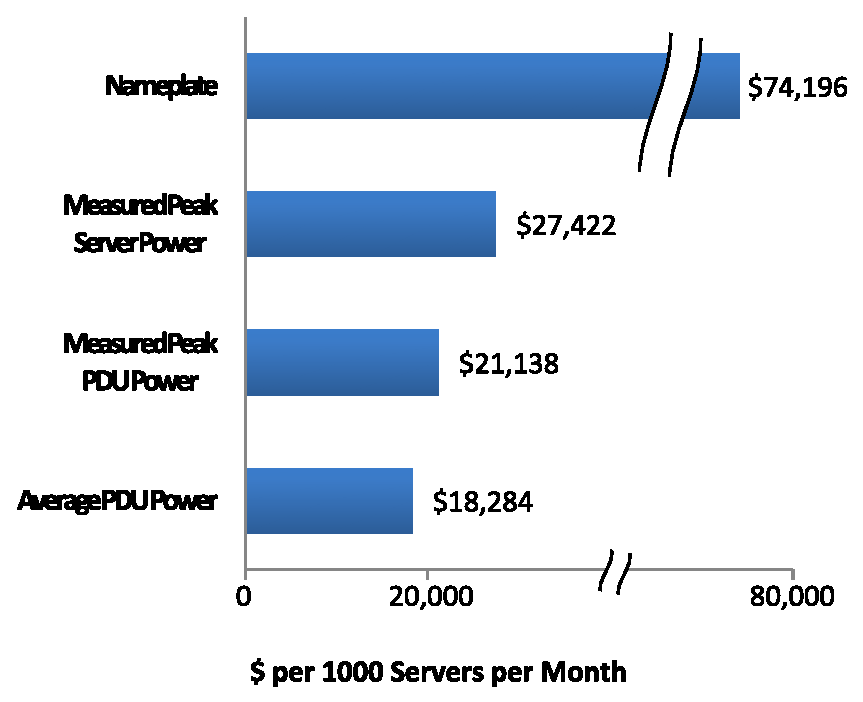
\includegraphics[width = 3.0 in]{Appendices/PowerRouting/figure/intro.eps}
\vspace{-.05 in}
\caption{ \textbf{The cost of over-provisioning.} \textnormal{Amortized monthly cost of power infrastructure for 1000 servers under varying provisioning schemes.}}
\label{figure::intro}
\vspace{-.1 in}
\end{figure}

Although the power demands of individual servers can vary greatly, statistical effects make it unlikely for all servers' demands to peak at the same time \cite{Govindan09,Ranganathan06}. Even in highly-tuned clusters running a single workload, peak utilization is rare, and still falls short of provisioned power capacity \cite{Fan07}.  This observation has lead researchers and operators to propose \emph{over-subscribing} power circuits.  To avoid overloads that might impact availability, such schemes rely on \emph{power capping} mechanisms that enforce power budgets at individual servers \cite{Lefurgy08, Wang08} or over ensembles \cite{Ranganathan06, Wang09}.  The most common power-capping approaches rely on throttling server performance to reduce power draw when budgets would otherwise be exceeded \cite{Lefurgy08,Ranganathan06, Wang08,Wang09}.  

Figure~\ref{figure::intro} illustrates the cost of conservative provisioning and the potential savings that can be gained by over-subscribing the power infrastructure.  The graph shows the amortized monthly capital cost for power infrastructure under varying provisioning schemes.  We calculate costs following the methodology of Hamilton \cite{Hamilton09} assuming high-availability power infrastructure costs \$15 per critical-load Watt \cite{Turner06}, the power infrastructure has a 15-year lifetime, and the cost of financing is 5\% per annum.   We derive the distribution of actual server power draws from 24 hours of data collected from 1000 servers in three production facilities (details in Section \ref{section::methodology}).  Provisioning power infrastructure based on nameplate ratings results in infrastructure costs over triple the facility's actual need.  Hence, operators typically ignore nameplate ratings, instead provisioning infrastructure based on a measured peak power for each class of server hardware.  However, even this provisioning method overestimates actual needs---provisioning based on the observed aggregate peak at any power distribution unit (PDU) reduces costs 23\%. Provisioning for less-than-peak loads can yield further savings at the cost of some performance degradation (e.g., average power demands are only 87\% of peak).  

Power capping makes over-subscribing safe.  However, power budgets must enforce local (PDU) as well as global (uninterruptible power supply, generator and utility feed) power constraints.  Hence, local spikes can lead to sustained performance throttling, even if the data center is lightly utilized and ample power delivery capacity is available elsewhere.  Moreover, in high-availability deployments, the need to maintain reserve capacity on redundant power delivery paths to ensure uninterrupted operation in the event of PDU failure magnifies the impact of utilization spikes---not only does the data center's direct demand rise, but also the potential load from failover.

An ideal power delivery system would balance loads across PDUs to ensure asymmetric demand does not arise.  Unfortunately, since server power demands vary, it is difficult or impossible to balance PDU loads statically, through clever assignment of servers to PDUs.  Such balancing may be achievable dynamically through admission control \cite{Chase01} or virtual machine migration \cite{Clark05}, but implies significant complexity, may hurt performance, and may not be applicable to non-virtualized systems. Instead, in this paper, we explore mechanisms to balance load through the \emph{power delivery infrastructure}, by dynamically connecting servers to PDUs. 

Our approach, \emph{Power Routing}, builds on widely-used techniques for fault-tolerant power delivery, whereby each server can draw power from either of two redundant feeds.  Rather than designating primary and secondary feeds and switching only on failure (or splitting loads evenly across both paths), we instead centrally control the switching of servers to feeds.  The soft-switching capability (already present  for ease of maintenance in many dual-corded power supplies and rack-level transfer switches) acts as the foundation of a power switching network.

In existing facilities, it is common practice for all servers in a rack or row to share the same pair of redundant power feeds, which makes it impossible to use soft-switching to influence local loading.  Our key insight, inspired by the notion of skewed-associative caches \cite{Seznec93} and declustering in disk arrays \cite{Alvarez98}), is to create \emph{shuffled distribution topologies}, where power feed connections are permuted among servers within and across racks. In particular, we seek topologies where servers running the same workload (which are most likely to spike together) connect to distinct pairs of feeds.  Such topologies have two implications.  First, they spread the responsibility to bear a failing PDU's load over a large number of neighbors, reducing the required reserve capacity at each PDU relative to conventional designs.  Second, they create the possibility, through a series of switching actions, to route slack in the power delivery system to a particular server.

Designing such topologies is challenging because similar servers tend to be collocated (e.g., because an organization manages ownership of data center space at the granularity of racks).  Shuffled topologies that route power from particular PDUs over myriad paths require wiring that differs markedly from current practice.  Moreover, assignments of servers to power feeds must not only meet PDU capacity constraints, they must also: (1) ensure that no overloads occur if any PDU fails (such a failure instantly causes all servers to switch to their alternate power feed); and (2) balance power draws across the three phases of each alternating current (AC) power source to avoid voltage and current fluctuations that increase heating, reduce equipment lifetime, and can precipitate failures \cite{Gruzs90}. Even given a shuffled topology, power routing remains challenging: we will show that solving the dynamic assignment of servers to PDUs reduces to the partitioning problem \cite{GareyBook}, and, hence, is NP-complete and infeasible to solve optimally.  In this paper, we address each of these challenges, to contribute:

\begin{packed_itemize}

\item {\bf Lower reserve capacity margins.}   Because more PDUs cooperate to tolerate failures, shuffled topologies reduce per-PDU capacity reserves from 50\% of instantaneous load to a $1/N$ fraction, where $N$ is the number of cooperating PDUs.   
\vspace{4pt}
\item {\bf Power routing.} We develop a linear programming-based heuristic algorithm that assigns each server a power feed and budget to minimize power capping, maintain redundancy against a single PDU fault, and balance power draw across phases.
\vspace{4pt}
\item {\bf Reduced capital expenses.}  Using traces from production systems, we demonstrate that our mechanisms reduce power infrastructure capital costs by 32\% without performance degradation.  With energy-proportional servers, savings reach 47\%.

\end{packed_itemize}

The rest of this paper is organized as follows.  In Section~\ref{section::background}, we provide background on data center power infrastructure and power capping mechanisms.   We describe our mechanisms in Section~\ref{section::powerrouting} and detail \PowerRouting's scheduling algorithm in Section~\ref{section::scheduling}.  We evaluate our techniques on our production data center traces in Section~\ref{section::evaluation}.  Finally, in Section~\ref{section::conclusion}, we conclude. 


% Background
\section{Background}
\label{section::background}

We begin with a brief overview of data center power provisioning infrastructure and power capping mechanisms.  A more extensive introduction to these topics is available in \cite{BarrosoBook09}.

\begin{figure*}[t]
\centering
\includegraphics[scale=.5]{Appendices/PowerRouting/figure/redundant.eps}
\vspace{-0.15 in}
\caption{ \textbf{Example power delivery system for a high-availability data center.} }
\vspace{-0.15 in}
\label{figure::redundant}
\end{figure*}


\textbf{Conventional power provisioning.} Today, most data centers operate according to power provisioning policies that assure sufficient capacity for every server. These policies are enforced by the data center operators at system installation time, by prohibiting deployment of any machine that creates the potential for overload.  Operators do their best to estimate systems' peak power draws, either through stress-testing, from vendor-supplied calculators, or through de-rating of nameplate specifications.

In high-availability data centers, power distribution schemes must also provision redundancy for fault tolerance; system deployments are further restricted by these redundancy requirements.  The Uptime Institute classifies data centers into tiers based on the nature and objectives of their infrastructure redundancy \cite{Turner05}. Some data centers provide no fault tolerance (Tier-1), or provision redundancy only within major power infrastructure components, such as the UPS system (Tier-2).  Such redundancy allows some maintenance of infrastructure components during operation, and protects against certain kinds of faults, but numerous single points-of-failure remain.  Higher-tier data centers provide redundant power delivery paths to each server. \PowerRouting is targeted at these data centers, as it exploits the redundant delivery paths to shift power delivery capacity.

\textbf{Example: A high-availability power system.} Figure~\ref{figure::redundant} illustrates an example of a high-availability power system design and layout for a data center with redundant distribution paths.  The design depicted here is based on the power architecture of the Michigan Academic Computer Center (MACC), the largest (10,000 square feet; 288 racks; 4MW peak load including physical infrastructure) of the three facilities providing utilization traces for this study. Utility power from two substations and a backup generator enter the facility at high voltage (13.2 kVAC) and meet at redundant automated transfer switches (ATS) that select among these power feeds.  These components are sized for the peak facility load (4MW), including all power infrastructure and cooling system losses.  The ATS outputs in turn are transformed to a medium voltage (480 VAC) and feed redundant uninterruptible power supply (UPS) systems, which are also each sized to support the entire facility.  These in turn provide redundant feeds to an array of power distribution units (PDUs) which further transform power to 208V 3-phase AC.  

PDUs are arranged throughout the data center such that each connects to two neighboring system clusters and each cluster receives redundant power feeds from its two neighboring PDUs.  The power assignments wrap from the last cluster to the first.  We refer to this PDU arrangement as a \emph{wrapped topology}. The wrapped topology provides redundant delivery paths with minimal wiring and requires each PDU to be sized to support  at most 150\% of the load of its connected clusters, with only a single excess PDU beyond the minimum required to support the load (called an ``N+1" configuration).  In the event of any PDU fault, 50\% of its supported load fails over to each of its two neighbors.  PDUs each support only a fraction of the data center's load, and can range in capacity from under ten to several hundred kilowatts.

Power is provided to individual servers through connectors (called ``whips"), that split the three phases of the 208VAC PDU output into the 120VAC single-phase circuits familiar from residential wiring.  (Some equipment may operate at higher voltages or according to other international power standards.) Many modern servers include redundant power supplies, and provide two power cords that can be plugged into whips from each PDU.  In such systems, the server internally switches or splits its load among its two power feeds.  For servers that provide only a single power cord, a rack-level transfer switch can connect the single cord to redundant feeds.

The capital costs of the power delivery infrastructure are concentrated at the large, high-voltage components: PDUs, UPSs, facility-level switches, generators, transformers and the utility feed.  The rack-level components cost a few thousand dollars per rack (on the order of \$1 per provisioned Watt), while the facility-level components can cost \$10-\$25 per provisioned Watt \cite{BarrosoBook09,Turner06}, especially in facilities with such high levels of redundancy.  With \PowerRouting, we focus on reducing the required provisioning of the facility-scale components while assuring a balanced load over the PDUs.  Though circuit breakers typically limit current both at the PDU's breaker panels and on the individual circuits in each whip, it is comparatively inexpensive to provision these statically to avoid overloads.  Though \PowerRouting is applicable to manage current limits on individual circuits, we focus on enforcing limits at the PDU level in this work.

\textbf{Phase balance}. In addition to enforcing current limits and redundancy, it is also desirable for a power provisioning scheme to balance power draw across the three phases of AC power supplied by each PDU.  Large phase imbalances can lead to current spikes on the neutral wire of a 3-phase power bus, voltage and current distortions on the individual phases, and generally increase heat dissipation and reduce equipment lifetime \cite{Gruzs90}.  Data center operators typically manually balance power draw across phases by using care in connecting equipment to particular receptacles wired to each phase.  \PowerRouting can automatically enforce phase balance by including it as explicit constraints in its scheduling algorithm. 


\textbf{Power capping.} Conservative, worst-case design invariably leads to power infrastructure over-provisioning \cite{Govindan09,Ranganathan06,Fan07,Wang09}.  Power capping mechanisms allow data center operators to sacrifice some performance in rare utilization spikes in exchange for substantial cost savings in the delivery infrastructure, without the risk of cascading failures due to an overload. In these schemes, some centralized control mechanism establishes a power budget for each server (e.g., based on historical predictions or observed load in the previous time epoch).  An actuation mechanism then enforces these budgets.  

\begin{figure*}[t]
\centering
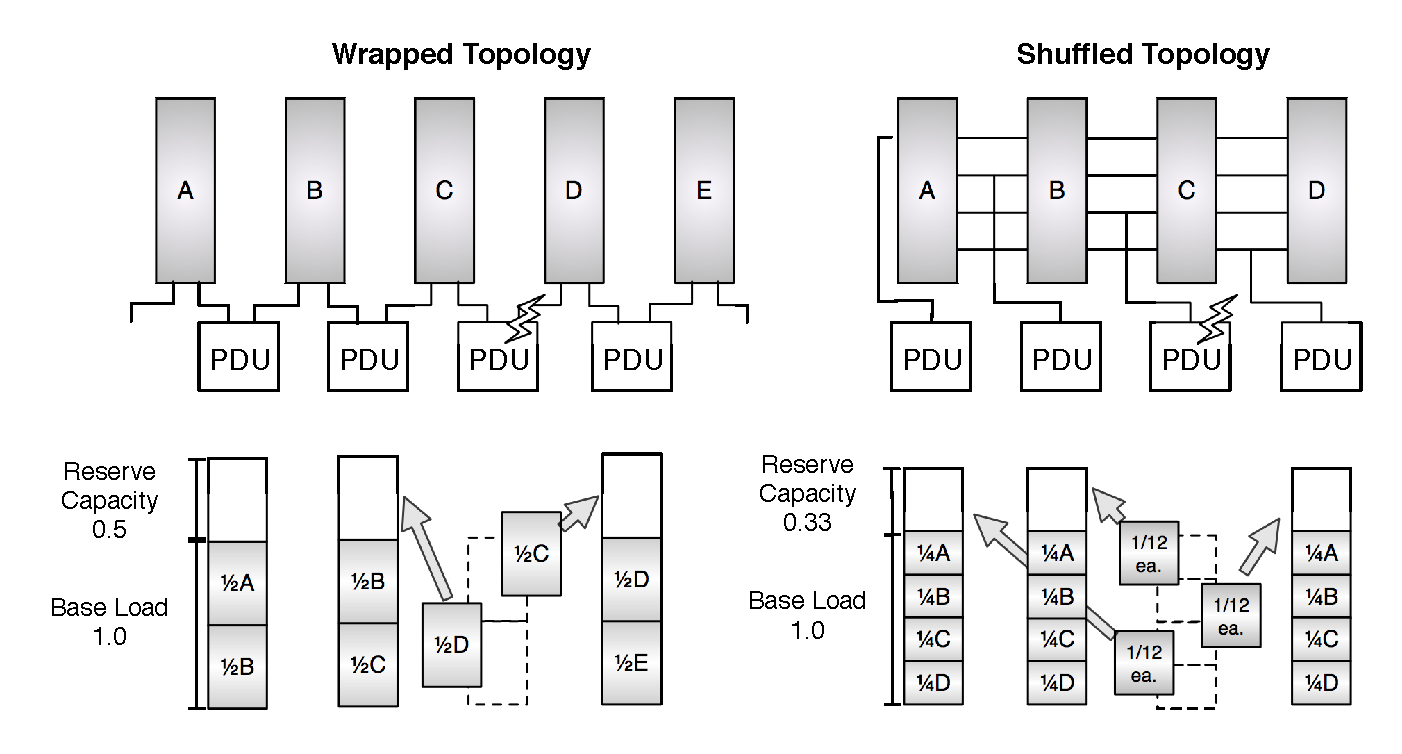
\includegraphics[width = 6.0 in]{Appendices/PowerRouting/figure/failover2.eps}
\caption{ \textbf{Reduced reserve capacity under shuffled topologies (4 PDUs, fully-connected topology).}}
\label{figure::failover}
\vspace{-.1 in}
\end{figure*}

The most common method of enforcing power budgets is through control loops that sense actual power draw and modulate processor frequency and voltage to remain within budget.  Commercial systems from IBM \cite{Popa06} and HP \cite{HP09} can enforce budgets to sub-watt granularities at milli-second timescales.  Researchers have extended these control mechanisms to enforce caps over multi-server chassis, larger ensembles, and entire clusters \cite{Ranganathan06,Lefurgy08,Wang08, Femal05}, examine optimal power allocation among heterogeneous servers \cite{Gandhi09b} and identify the control stability challenges when capping at multiple levels of the power distribution hierarchy \cite{Raghavendra08,Wang09}. Others have examined extending power management to virtualized environments \cite{Nathuji07}.  Soft fuses \cite{Govindan09} apply the notion of power budgets beyond the individual server and enforce sustained power budgets, which allow for transient overloads that the power infrastructure can support.  Finally, prior work considers alternative mechanisms for enforcing caps, such as modulating between active and sleep states \cite{Gandhi09a}. 

Like prior work, \PowerRouting relies on a power capping mechanism as a safety net to ensure extended overloads can not occur.  However, \PowerRouting is agnostic to how budgets are enforced. For simplicity, we assume capping based on dynamic frequency and voltage scaling, the dominant approach.  

Though rare, peak utilization spikes do occur in some facilities.  In particular, if a facility runs a single distributed workload balanced over all servers (e.g., as in a web search cluster), then the utilization of all servers will rise and fall together \cite{Fan07}.  No scheme that over-subscribes the physical infrastructure can avoid performance throttling for such systems. The business decision of whether throttling is acceptable in these rare circumstances is beyond the scope of this study; however, for any given physical infrastructure budget, \PowerRouting reduces performance throttling relative to existing capping schemes, by shifting loads among PDUs to locate and exploit spare capacity.



% Design
\section{Power Routing.}
\label{section::powerrouting}


\PowerRouting relies on two central concepts.  First, it exploits \emph{shuffled topologies} for power distribution to increase the connectivity between servers and diverse PDUs.  Shuffled topologies spread responsibility to sustain the load on a failing PDU, reducing the required reserve capacity per PDU.  Second, \PowerRouting relies on a \emph{scheduling} algorithm to assign servers' load across redundant distribution paths while balancing loads over PDUs and AC phases.  When loads are balanced, the provisioned capacity of major power infrastructure components (PDUs, UPSs, generators, and utility feeds) can be reduced, saving capital costs.  We first detail the design and advantages of shuffled topologies, and then discuss \PowerRouting.

\subsection{Shuffled Topologies.}
\label{section::intermixed}

\begin{figure*}[t]
\centering
\subfigure[Wrapped (conventional)]{
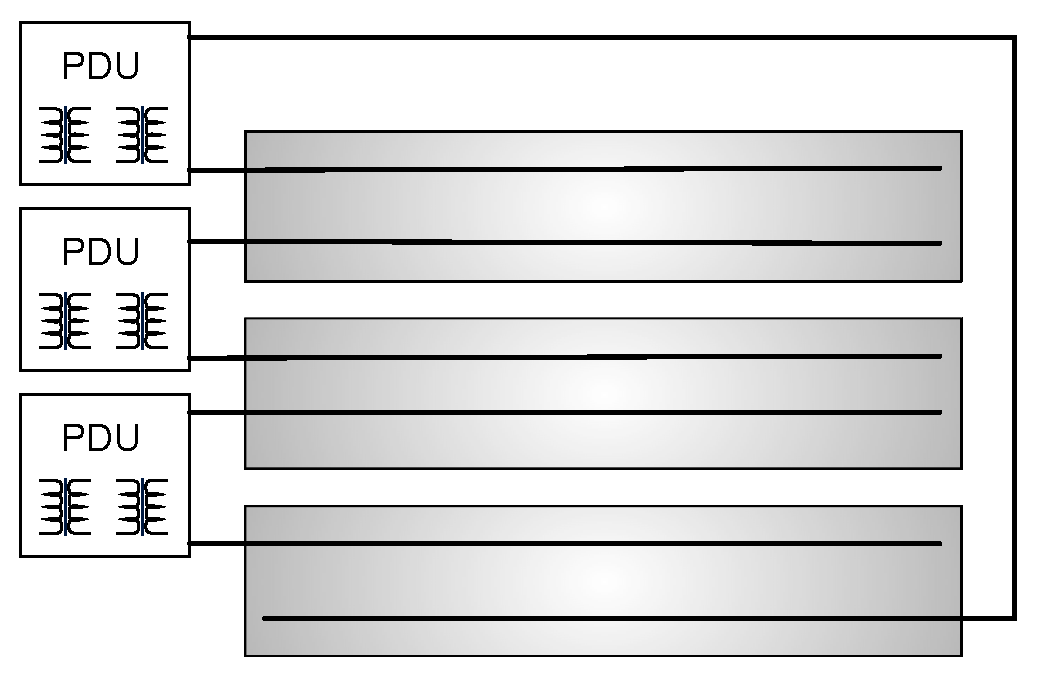
\includegraphics[scale=.3]{Appendices/PowerRouting/figure/standard3.eps}
\label{figure::wrapped}
}
\hspace{0.3in}
\subfigure[Fully-connected]{
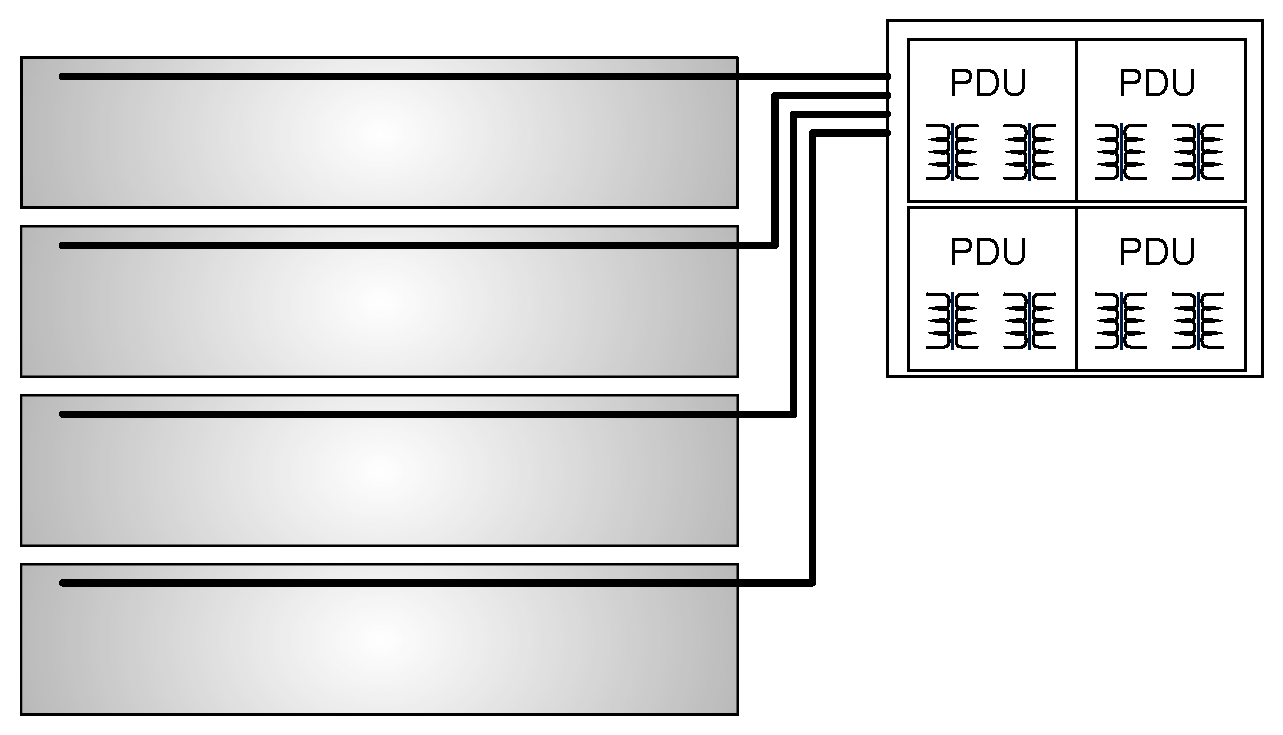
\includegraphics[scale=.3]{Appendices/PowerRouting/figure/full2.eps}
\label{figure::connected}
}
\qquad
\subfigure[Serpentine]{
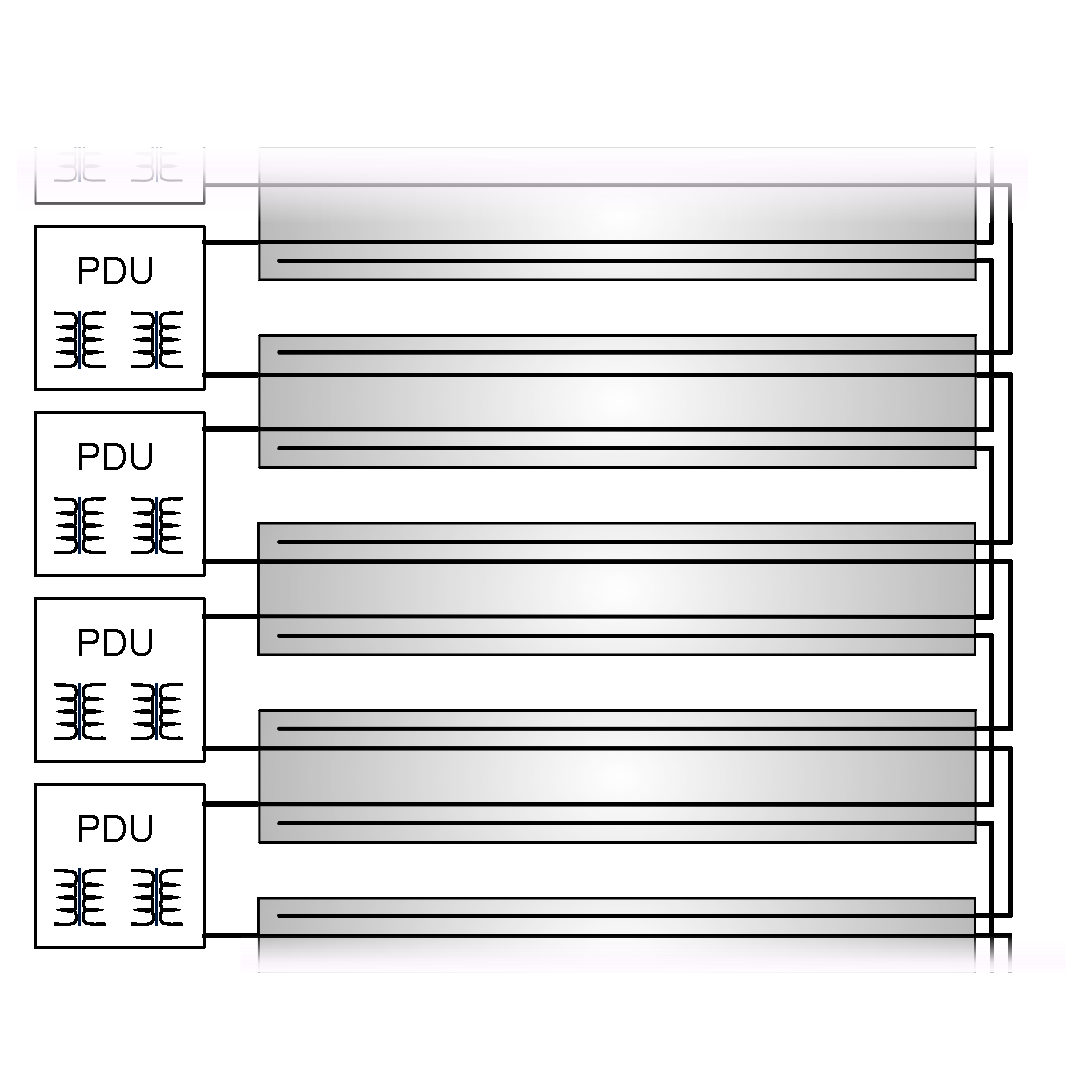
\includegraphics[scale=.3]{Appendices/PowerRouting/figure/ring.eps}
\label{figure::ring}
}
\hspace{0.5in}
\subfigure[X-Y]{
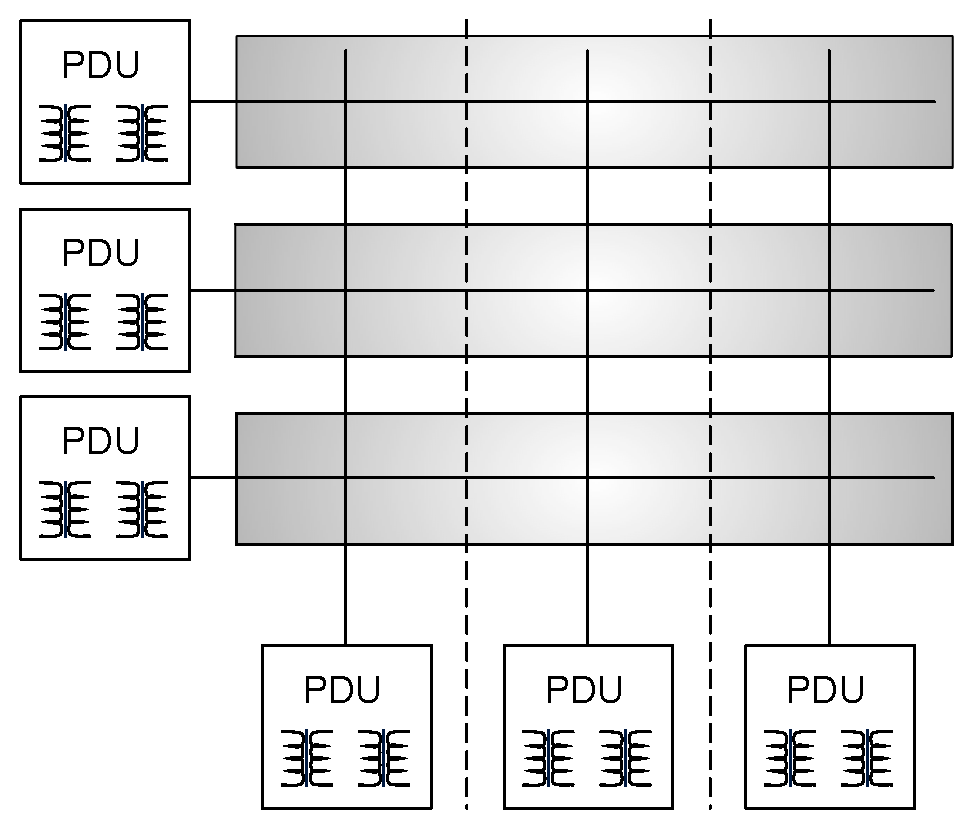
\includegraphics[scale=.3]{Appendices/PowerRouting/figure/xy3.eps}
\label{figure::xy}
}

\vspace{-0.10 in}
\caption{ \textbf{Shuffled power distribution topologies.} }
\vspace{-0.15 in}
\label{figure::topologies}
\end{figure*}

In high-availability data centers, servers are connected to two PDUs to ensure uninterrupted operation in the event of a PDU fault.  A naive (but not unusual) connection topology provisions paired PDUs for each cluster of machines.  Under this data center design, each PDU must be sized to support the full worst-case load of the entire cluster; hence, the power infrastructure is 50\% utilized in the best case. As described in Section~\ref{section::background}, the more sophisticated ``wrapped" topology shown in Figure~\ref{section::background} splits a failed PDU's load over two neighbors, allowing each PDU to be sized to support only 150\% of its nominal primary load.  

By spreading the responsibility for failover further, to additional PDUs, the spare capacity required of each PDU can be reduced---the more PDUs that cooperate to cover the load of a failed PDU, the less reserve capacity is required in the data center as a whole.  In effect, the reserve capacity in each PDU protects multiple loads (which is acceptable provided there is only a single failure). 

Figure~\ref{figure::failover} illustrates the differing reserve capacity requirements of the wrapped topology and a shuffled topology where responsibility for reserve capacity is spread over three PDUs.  The required level of reserve capacity at each PDU is approximately $X / N$, where $X$ represents the cluster power demand, and $N$ the number of PDUs cooperating to provide reserve capacity. (Actual reserve requirements may vary depending on the instantaneous load on each phase).

The savings from shuffled topologies do not require any intelligent switching capability; rather, they require only increased diversity in the distinct combinations of primary and secondary power feeds for each server (ideally covering all combinations equally).   

The layout of PDUs and power busses must be carefully considered to yield feasible shuffled wiring topologies.   Our distribution strategies rely on overhead power busses \cite{Rasmussen129} rather than conventional under-floor conduits to each rack.  The power busses make it easier (and less costly) to connect many, distant racks to a PDU.  Power from each nearby bus is routed to a panel at the top of each rack, and these in turn connect to vertical whips (i.e., outlet strips) that supply power to individual servers.  The whips provide outlets in pairs (or a single outlet with an internal transfer switch) to make it easy to connect servers while assuring an appropriate mix of distinct primary and secondary power feed combinations.

Though overhead power busses are expensive, they still account for a small fraction of the cost of large-scale data center power infrastructure.  Precise quantification of wiring costs is difficult without detailed facility-specific architecture and engineering. We neglect differences in wiring costs when estimating data center infrastructure costs, and instead examine the (far more significant) impact that topologies have on the capacity requirements of the high-voltage infrastructure.  The primary difficulty of complex wiring topologies lies in engineering the facility-specific geometry of the large (and dangerous) high-current overhead power rails; a challenge that we believe is surmountable.

We propose three shuffled power distribution topologies that improve on the wrapped topology of current high-availability data centers.  The \emph{fully connected} topology collocates all PDUs in one corner of the room, and routes power from all PDUs throughout the entire facility.  This topology is not scalable. However, we study it as it represents an upper bound on the benefits of shuffled topologies. We further propose two practical topologies.  The \emph{X-Y} topology divides the data center into a checkerboard pattern of power zones, routing power both north-south and east-west across the zones.  The \emph{serpentine} topology extends the concept of the wrapped topology (see Figure~\ref{figure::redundant}) to create overlap among neighboring PDUs separated by more than one row.

Each distribution topology constrains the set of power feed combinations available in each rack in a different manner.  These constraints in turn affect the set of choices available to the \PowerRouting scheduler, thereby impacting its effectiveness.  


\textbf{Wrapped Topology}.  Figure~\ref{figure::wrapped} illustrates the wrapped topology, which is our term for the conventional  high-availability data center topology (also seen in Figure~\ref{figure::redundant}).  This topology provides limited connectivity to PDUs, and is insufficient for \PowerRouting. 

\textbf{Fully-connected Topology}.  Figure~\ref{figure::connected} illustrates the fully-connected topology.  Under this topology, power is routed from every PDU to every rack. As noted above, the fully-connected topology does not scale and is impractical in all but the smallest data centers.  However, one scalable alternative is to organize the data center as disconnected islands of fully-connected PDUs and rack clusters.  Such a topology drastically limits \PowerRouting flexibility, but can scale to arbitrary-sized facilities.

\textbf{Serpentine Topology}.  Figure~\ref{figure::ring} illustrates the serpentine topology.  Under this topology, PDUs are located at one end of the data centers' rows, as in the wrapped topology shown in Figure~\ref{figure::redundant}.  However, whereas in the wrapped topology a power bus runs between two equipment rows from the PDU to the end of the facility, in the serpentine topology, the power bus then bends back, returning along a second row.  This snaking bus pattern is repeated for each PDU, such that two power busses run in each aisle and four busses are adjacent to each equipment row.  The pattern scales to larger facilities by adding PDUs and replicating the pattern over additional rows.  It scales to higher PDU connectivity by extending the serpentine pattern with an additional turn.

\textbf{X-Y Topology}.  Figure~\ref{figure::xy} illustrates the X-Y topology. Under this topology, the data center is divided into square zones in a checkerboard pattern.  PDUs are located along the north and west walls of the data center.  Power busses from each PDU route either north-south or east-west along the centerline of a row (column) of zones.  Hence, two power busses cross in each zone.  These two busses are connected to each rack in the zone. This topology scales to larger facilities in a straight-forward manner, by adding zones to the ``checkerboard."  It scales to greater connectivity by routing power busses over the zones in pairs (or larger tuples).



\subsection{Power Routing.}

\PowerRouting leverages shuffled topologies to achieve further capital cost savings by under-provisioning PDUs relative to worst-case demand.   The degree of under-provisioning is a business decision made at design time (or when deploying additional systems) based on the probability of utilization spikes and the cost of performance throttling (i.e., the risk of failing to meet a service-level agreement).  \PowerRouting shifts spare capacity to cover local power demand spikes by controlling the assignment of each server to its primary or secondary feed.  The less correlation there is among spikes, the more effective \PowerRouting will be at covering those spikes by shifting loads rather than throttling performance.  \PowerRouting relies on a capping mechanism to prevent overloads when spikes cannot be covered.

\PowerRouting employs a centralized control mechanism to assign each server to its primary or secondary power feed and set power budgets for each server to assure PDU overloads do not occur.  Each time a server's power draw increases to its pre-determined cap (implying that performance throttling will be engaged), the server signals the \PowerRouting controller to request a higher cap.  If no slack is available on the server's currently active power feed, the controller invokes a scheduling algorithm (detailed in Section~\ref{section::scheduling}) to determine new power budgets and power feed assignments for all servers to try to locate slack elsewhere in the power distribution system.  The controller will reduce budgets for servers whose utilization has decreased and may reassign servers between their primary and secondary feeds to create the necessary slack.  If no solution can be found (e.g., because aggregate power demand exceeds the facilities' total provisioning), the existing power cap remains in place and the server's performance is throttled.  

In addition to trying to satisfy each server's desired power budget, the \PowerRouting scheduler also maintains sufficient reserve capacity at each PDU to ensure continued operation (under the currently-established power budgets) even if any single PDU fails.  A PDU's required reserve capacity is given by the largest aggregate load served by another PDU for which it acts as the secondary (inactive) feed.

Finally, the \PowerRouting scheduler seeks to balance load across the three AC phases of each PDU.  As noted in Section~\ref{section::background}, phase imbalance can lead to numerous electrical problems that impact safety and availability.  The scheduler constrains the current on each of the three phases to remain within a 20\% margin.

The key novelty of \PowerRouting lies in the assignment of servers to power feeds; sophisticated budgeting mechanisms (e.g., which assign asymmetric budgets to achieve higher-level QoS goals) have been extensively studied \cite{Ranganathan06,Lefurgy08,Wang08, Femal05,Raghavendra08,Wang09,Nathuji07,Gandhi09b}.  Hence, in this paper, we focus our design and evaluation on the power feed scheduling mechanism and do not explore QoS-aware capping in detail.

\subsection{Implementation.}

\PowerRouting comprises four elements: (1) an actuation mechanism to switch servers between their two redundant power feeds; (2) the centralized controller that executes the power feed scheduling algorithm;  (3) a communications mechanism for the controller to direct switching activity and assign budgets; and (4) a power distribution topology that provisions primary and secondary power feeds in varying combinations to the receptacles in each rack.   

\textbf{Switching power feeds}. The power feed switching mechanism differs for single- and dual-corded servers.  In a single-corded server, an external transfer switch attaches the server to its primary or secondary power feed.  In the event of a power interruption on the active feed, the transfer switch seamlessly switches the load to the alternative feed (a local, automatic action).  The scheduler assures that all PDUs have sufficient reserve capacity to supply all loads that may switch to them in the event of any single PDU failure.  To support phase balancing, the transfer switch must be capable of switching loads across out-of-phase AC sources fast enough to appear uninterrupted to computer power supplies.  External transfer switches of this sort are in wide-spread use today, and retail for several hundred dollars. In contrast to existing transfer switches, which typically switch entire circuits (several servers), \PowerRouting requires switching at the granularity of individual receptacles, implying somewhat higher cost. For dual-corded servers, switching does not require any additional hardware, as the switching can be accomplished through the systems' internal power supplies. 

\textbf{Control unit}. The \PowerRouting control unit is a microprocessor that orchestrates the power provisioning process.  Each time scheduling is invoked, the control unit performs four steps: (1) it determines the desired power budget for each server; (2) it schedules each server to its primary or secondary power feed; (3) it assigns a power cap to each server (which may be above the request, allowing headroom for utilization increase, or below, implying performance throttling); and (4) it communicates the power cap and power feed assignments to all devices.  The control unit can be physically located within the existing intelligence units in the power delivery infrastructure (most devices already contain sophisticated, network-attached intelligence units). Like other power system components, the control unit must include mechanisms for redundancy and fault tolerance.  Details of the control unit's hardware/software fault tolerance are beyond the scope of this study; the challenges here mirror those of the existing intelligence units in the power infrastructure.  

The mechanisms used in each of the control unit's four steps are orthogonal. As this study is focused on the novel scheduling aspect of \PowerRouting (step 2), we explore only relatively simplistic policies for the other steps.  We determine each server's desired power budget based in its peak demand in the preceding minute.  Our power capping mechanism assigns power budgets that throttle servers to minimize the total throttled power.
%\fixme{Add a comment citing work with more intelligent capping policies.}

\textbf{Communication.} Communication between the control unit and individual servers/transfer switches is best accomplished over the data center's existing network infrastructure, for example, using the Simple Network Management Protocol (SNMP) or BACnet.  The vast majority of power provisioning infrastructure already supports these interfaces.  Instantaneous server power draws and power budgets can also typically be accessed through SNMP communication with the server's Integrated Lights Out (ILO) interface. 

\textbf{Handling uncontrollable equipment.} Data centers contain myriad equipment that draw power, but cannot be controlled by \PowerRouting (e.g., network switches, monitors).  The scheduler must account for the worst-case power draw of such equipment when calculating available capacity on each PDU and phase.

\begin{figure}[b]
\centering
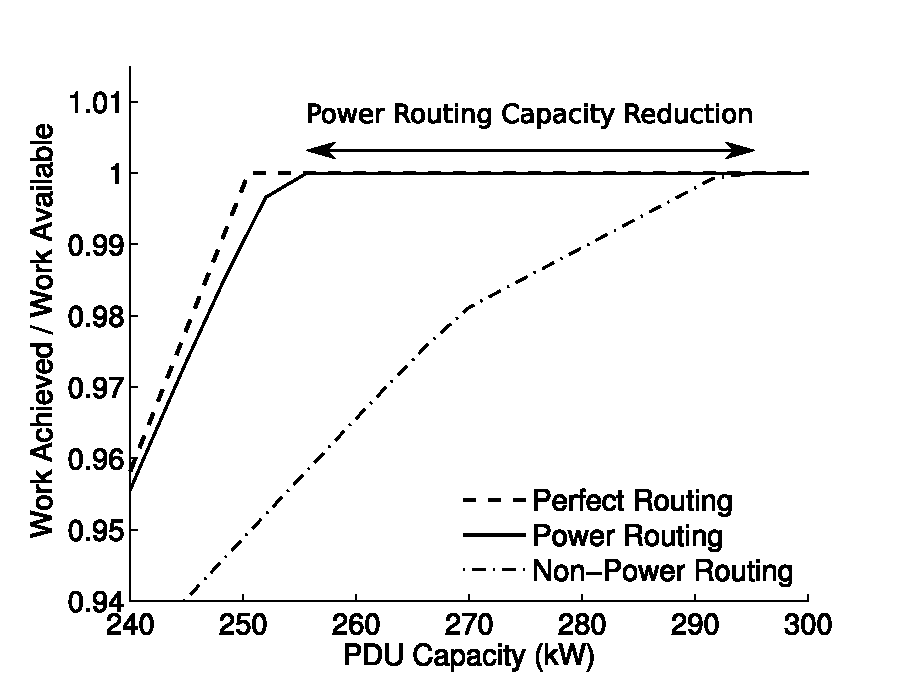
\includegraphics[width = 3.0 in]{Appendices/PowerRouting/figure/RoutingComparison.eps}
\caption{ \textbf{Shuffled Topologies: 6 PDUs, fully-connected}}
\label{figure::routingdemonstration}
\vspace{-.1 in}
\end{figure}

\subsection{Operating Principle.}

\PowerRouting relies on the observation that individual PDUs are unlikely to reach peak load simultaneously.
The power distribution system as a whole operates in one of three regimes.
The first, most common case is that the load on all PDUs is below their capacity.  In this case, the power infrastructure is over-provisioned, power capping is unnecessary, and the entire data center operates at full performance. At the opposite extreme, when servers demand more power than is available, the power infrastructure is under-provisioned, all PDUs will be fully loaded, and power capping (e.g., via performance throttling) is necessary.  In either of these regimes, \PowerRouting has no impact; the power infrastructure is simply under- (over-) provisioned relative to the server demand. 

\PowerRouting is effective in the intermediate regime where some PDUs are overloaded while others have spare capacity.  In current data centers, this situation will result in performance throttling that \PowerRouting can avoid.

To illustrate how \PowerRouting affects performance throttling, we explore its performance envelope near the operating region where aggregate power infrastructure capacity precisely meets demand.  Figure~\ref{figure::routingdemonstration} shows the relationship between installed PDU capacity and performance throttling (in terms of the fraction of offered load that is met) with and without  \PowerRouting (6 PDUs, fully-connected topology) and contrast these against an ideal, perfectly-balanced power distribution infrastructure.    The ideal infrastructure can route power from any PDU to any server and can split load fractionally over multiple PDUs.  (We detail the methodology used to evaluate \PowerRouting and produce these results in Section~\ref{section::methodology} below.)

The graph provides two insights into the impact of \PowerRouting.  First, we can use it to determine how much more performance \PowerRouting achieves for a given infrastructure investment relative to conventional and ideal designs.  This result can be obtained by comparing vertically across the three lines for a selected PDU capacity. As can be seen, \PowerRouting closely tracks the performance of the ideal power delivery infrastructure, recovering several percent of lost performance relative to a fully-connected topology without power routing.

The graph can also be used to determine the capital infrastructure savings that \PowerRouting enables while avoiding performance throttling altogether.  Performance throttling becomes necessary at the PDU capacity where each of the three power distributions dips below 1.0.  The horizontal distance between these intercepts is the capacity savings, and is labeled  ``Power Routing Capacity Reduction" in the figure. In the case shown here, \PowerRouting avoids throttling at a capacity of 255 kW, while 294 kW of capacity are needed without \PowerRouting. \PowerRouting avoids throttling, allowing maximum performance with less investment in power infrastructure.


% Scheduling
\section{Scheduling}
\label{section::scheduling}

\PowerRouting relies on a centralized scheduling algorithm to assign power to servers. Each time a server requests additional power (as a result of exhausting its power cap) the scheduler checks if the server's current active power feed has any remaining capacity, granting it if possible. If no slack exists, the scheduler attempts to create a new allocation schedule for the entire facility that will eliminate or minimize the need for capping. In addition to considering the actual desired power budget of each server, the scheduler must also provision sufficient reserve capacity on each feed such that the feed can sustain its share of load if any PDU fails.  Finally, we constrain the scheduler to allow only phase-balanced assignments where the load on the three phases of any PDU differ by no more than 20\% of the per-phase capacity.

The scheduling process comprises three steps: gathering the desired budget for each server, solving for an assignment of servers to their primary or secondary feeds, and then, if necessary, reducing server's budgets to meet the capacity constraints on each feed.

Whereas sophisticated methods for predicting power budgets are possible \cite{Choi08}, we use a simple policy of assigning each server a budget based on its average power demand in the preceding minute.  More sophisticated mechanisms are orthogonal to the scheduling problem itself.

Solving the power feed assignment problem optimally, even without redundancy, is an NP-Complete problem.  It is easy to see that power scheduling $\in$ NP; a nondeterministic algorithm can enumerate a set of assignments from servers to PDUs and then check in polynomial time that each PDU is within its power bounds.  To show that power scheduling is NP-Complete we transform PARTITION to it \cite{GareyBook}.  For a given instance of PARTITION of finite set $A$ and a size $s(a) \in \field{Z+}$ for each $a \in A$: we would like to determine if there is a subset $A' \in A$ such that the $\sum_{a \in A'}{s(a)} = \sum_{a \in A-A'}{s(a)}$. Consider $A$ as the set of servers, with $s(a)$ corresponding to server power draw. Additionally consider two PDUs each of power capacity $\sum_{a} s(a) / 2$. These two problems are equivalent. Thus, a polynomial time solution to power scheduling will yield a polynomial time solution to PARTITION (implying power scheduling is NP-Complete).

In data centers of even modest size, brute force search for an optimal power feed assignment is infeasible.  Hence, we resort to a heuristic approach to generate an approximate solution.  

We first optimally solve a power feed assignment problem allowing servers to be assigned fractionally across feeds using linear programming.  This linear program can be solved in polynomial time using standard methods \cite{CormenBook}. From the exact fractional solution, we then construct an approximate solution to the original problem (where entire servers must be assigned a power feed).  Finally, we check if the resulting assignments are below the capacity of each power feed.  If any feed's capacity is violated, we invoke a second optimization step to choose power caps for all servers.  

Determining optimal caps is non-trivial because of the interaction between a server's power allocation on its primary feed, and the reserve capacity that allocation implies on its secondary feed.  We employ a second linear programming step to determine a capping strategy that maximizes the amount of power allocated to servers (as opposed to reserve capacity).

{\bf Problem formulation.} We formulate the linear program based on the power distribution topology (i.e., the static assignment of primary and secondary feeds to each server), the desired server power budgets, and the power feed capacities.  For each pair of power feeds we calculate $Power_{i,j}$, the sum of power draws for all servers connected to feeds $i$ and $j$. (Our algorithm operates at the granularity of individual phases of AC power from each PDU, as each phase has limited ampacity). $Power_{i,j}$ is 0 if no server shares feeds  $i$ and $j$ (e.g., if the two feeds are different phases from the same PDU or no server shares those PDUs).  Next, for each pair of feeds, we define variables $Feed_{i,j}i$ and $Feed_{i,j}j$ to account for the server power from $Power_{i,j}$ routed to feeds $i$ and $j$, respectively.  Finally, a single global variable, $Slack$, represents the maximum unallocated power on any phase after all assignments are made.  
With these definitions, the linear program maximizes $Slack$ subject to the following constraints:

$\forall i, j \neq i$, $i$ and $j$ are any phases on different PDUs:

\vspace{-.2 in}
\begin{equation}\label{rationalbin}
Feed_{i,j}i + Feed_{i,j}j = Power_{i,j}
\end{equation}

\vspace{-.25 in}
\begin{equation}\label{pducapacity}
\displaystyle\sum_{k \neq i} Feed_{i,k}i + \displaystyle\sum_{l in j's PDU} Feed_{i,l}l + Slack \le Capacity(i) 
\end{equation}
\vspace{-.15 in}

And constraints for distinct phases $i$ and $j$ within a single PDU:

\vspace{-.2 in}
\begin{equation}\label{phasebalance}
|\displaystyle\sum_{k \neq i} Feed_{i,k}i - \displaystyle\sum_{k \neq j} Feed_{j,k}j| \le .2 \times Capacity(i,j)
\end{equation}
\vspace{-.15 in}

With the following bounds:

\vspace{-.2 in}
\begin{equation}\label{freeslack}
-\infty \le Slack \le \infty
\end{equation}
\vspace{-.15 in}

\vspace{-.25 in}
\begin{equation}\label{positivefeeds}
\forall i, j \ne i : Feed_{i,j}i, Feed_{i,j}j \ge 0
\end{equation}
\vspace{-.15 in}

Equation \ref{rationalbin} ensures that power from servers connected to feeds $i$ and $j$ is assigned to one of those two feeds.
Equation \ref{pducapacity} restricts the sum of all power assigned to a particular feed $i$, plus the reserve capacity required on $i$ should feeds on  $j$'s PDU fail, plus the excess slack to be less than the capacity of feed $i$. Finally, equation \ref{phasebalance} ensures that phases are balanced across each PDU. A negative $Slack$ indicates that more power is requested by servers than is available (implying that there is no solution to the original, discrete scheduling problem without power capping).

We use the fractional power assignments from the linear program to schedule servers to feeds.
For a given set of servers, $s$, connected to both feed $i$ and feed $j$, the fractional solution will indicate that $Feed_{i,j}i$ watts be assigned to $i$ and $Feed_{i,j}j$ to $j$.  The scheduler must create a discrete assignment of servers to feeds to approximate the desired fractional assignments as closely as possible, which is itself a bin packing problem.  To solve this sub-problem efficiently, the scheduler sorts the set $s$ descending by power and repeatedly assign the largest unassigned server to $i$ or $j$, whichever has had less power assigned to it thus far (or whichever has had less power relative to its capacity if the capacities differ).

If a server cannot be assigned to either feed without violating the feed's capacity constraint, then throttling may be necessary to achieve a valid schedule.  The server is marked as ``pending" and left temporarily unassigned. By the nature of the fractional solution, at most one server in the set can remain pending.  This server must eventually be assigned to one of the two feeds; the difference between this discrete assignment and the optimal fractional assignment is the source of error in our heuristic. By assigning the largest servers first we attempt to minimize this error. Pending servers will be assigned to the feed with the most remaining capacity once all other servers have been assigned.

The above optimization algorithm assumes that each pair of power feeds shares several servers in common, and that the power drawn by each server is much less than the capacity of the feed.
We believe that plausible power distribution topologies fit this restriction.

Following server assignment, if no feed capacity constraints have been violated, the solution is complete and all servers are assigned caps at their requested budgets.  If any slack remains on a feed, it can be granted upon a future request without re-invoking the scheduling mechanism, avoiding unnecessary switching. 

If any capacity constraints have been violated, a new linear programming problem is formulated to select power caps that maximize the amount of power allocated to servers (as opposed to reserve capacity for fail-over).  We scale back each feed such that no PDU supplies more power than its capacity, even in the event that another PDU fails.  The objective function maximizes the sum of the server budgets.  We assume that servers can be throttled to any frequency from idle to peak utilization and that the relationship and limits of frequency and power scaling are known a priori.
Note, however, that this formulation ignores heterogeneity in power efficiency, performance, or priority across servers; it considers only the redundancy and topology constraints of the power distribution network.  An analysis of more sophisticated mechanisms for choosing how to cap servers that factors in these considerations is outside the scope of this paper.



% Evaluation
\section{Evaluation}
\label{section::evaluation}

Our evaluation demonstrates the effectiveness of shuffled topologies and \PowerRouting at reducing the required capital investment in power infrastructure to meet a high-availability data center's reliability and power needs.  First, we demonstrate how shuffled topologies reduce the reserve capacity required to provide single-PDU-fault tolerance.  Then, we examine the effectiveness of \PowerRouting at further reducing provisioning requirements as a function of topology, number of PDUs, and workload.  Finally, we show how \PowerRouting will increase in effectiveness as server power management becomes more sophisticated and the gap between servers' idle and peak power demands grows.

\subsection{Methodology}
\label{section::methodology}

We evaluate \PowerRouting through analysis of utilization traces from a large collection of production systems. We simulate \PowerRouting's scheduling algorithm and impact on performance throttling and capital cost.

{\bf Traces.}
We collect utilization traces from three production facilities: (1) \emph{EECS servers}, a small cluster of departmental servers (web, email, login, etc.) operated by the Michigan EECS IT staff; (2) \emph{Arbor Lakes Data Center}, a ~1.5MW facility supporting the clinical operations of the University of Michigan Medical Center; and (3) \emph{Michigan Academic Computer Center (MACC)}, a 4MW high-performance computing facility operated jointly by the University of Michigan, Internet2, and Merit that runs primarily batch processing jobs.  These sources provide a diverse mix of real-world utilization behavior.  Each of the traces ranges in length from three to forty days sampling server utilization once per minute.  We use these traces to construct a hypothetical high-availability hosting facility  comprising 400 medical center servers, 300 high performance computing nodes, and a 300-node web search cluster.   The simulated medical center and HPC cluster nodes each replay a trace from a specific machine in the corresponding real-world facility.  The medical center systems tend to be lightly loaded, with one daily utilization spike (which we believe to be daily backup processing).  The HPC systems are heavily loaded.  As we do not have access to an actual 300-node web search cluster, we construct a cluster by replicating the utilization trace of a single production web server over 300 machines.  The key property of this synthetic search cluster is that the utilization on individual machines rises and falls together in response to user traffic, mimicking the behavior reported for actual search clusters \cite{Fan07}.  We analyze traces for a 24-hour period. Our synthetic cluster sees a time-average power draw of 180.5 kW, with a maximum of 208.7 kW and standard deviation of 9 kW.

{\bf Power.}  We convert utilization traces to power budget requests using published SPECPower results \cite{SpecPower}.  Most of our traces have been collected from systems where no SPECPower result has been published; for these, we attempt to find the closest match based on vendor descriptions and the number and model of CPUs and installed memory. As SPECPower only provides power at intervals of 10\% utilization, we use linear interpolation to approximate power draw in between these points.

Prior work \cite{Fan07,Ranganathan06} has established that minute-grained CPU utilization traces can predict server-grain power 
draw to within a few percent.   Because of the scope of our data collection efforts, finer-grained data collection is impractical.  Our estimates of savings from Power Routing are conservative; finer-grained scheduling might allow tighter tracking of instantaneous demand.  

To test our simulation approach, we have validated simulation-derived power values against measurements of individual servers in our lab.    Unfortunately, the utilization and power traces available from our production facilities are not exhaustive, which precludes a validation experiment where we compare simulation-derived results to measurements for an entire data center.
 
{\bf Generating data center topologies.} For each power distribution topology described in Section~\ref{section::intermixed}, we design a layout of our hypothetical facility to mimic the typical practices seen in the actual facilities. We design layouts according to the policies the Michigan Medical Center IT staff use to manage their \emph{Arbor Lakes} facility. Each layout determines an assignment of physical connections from PDUs to servers. Servers that execute similar applications are collocated in the same rack, and, hence, in conventional power delivery topologies, are connected to the same PDU.  Where available, we use information about the actual placement of servers in racks to guide our placement.  Within a rack, servers are assigned across PDU phases in a round-robin fashion.  We attempt to balance racks across PDUs and servers within racks across AC phases based on the corresponding system's power draw at 100\% utilization.  No server is connected to two phases of the same PDU, as this arrangement does not protect against PDU failure.  We use six PDUs in all topologies unless otherwise noted.

{\bf Metrics.} We evaluate \PowerRouting based on its impact on server throttling activity and data center capital costs.  As the effect of voltage and frequency scaling on performance varies by application, we instead use the fraction of requested server power budget that was not satisfied as a measure of the performance of capping techniques.  Under this metric, the ``cost" of failing to supply a watt of requested power is uniform over all servers, obviating the need to evaluate complex performance-aware throttling mechanisms (which are orthogonal to \PowerRouting). Our primary evaluation metric is the minimum total power delivery capacity required to assure zero performance throttling, as this best illustrates the advantage of \PowerRouting over conventional worst-case provisioning.

\subsection{Impact of Shuffled Topologies}

\begin{figure}[t!]
\centering
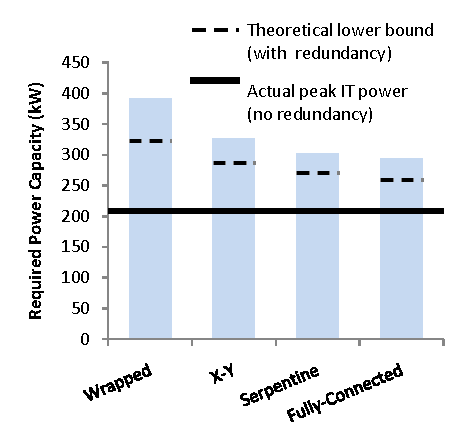
\includegraphics[width = 3.0 in]{Appendices/PowerRouting/figure/result_intermix.eps}
\caption{ \textbf{Minimum capacity for redundant operation under shuffled topologies (no Power Routing).} }
\label{figure::intermix}
\vspace{-.1 in}
\end{figure}

We first compare the impact of shuffled topologies on required power infrastructure capacity.  Shuffled topologies reduce the reserve capacity that each PDU must sustain to provide fault tolerance against single-PDU failure.  We examine the advantage of several topologies relative to the baseline high-availability ``wrapped" data center topology, which requires each PDU to be over-provisioned by 50\% of its nominal load.  We report the total power capacity required to prevent throttling for our traces.  We assume that each PDU must maintain sufficient reserve capacity at all times to precisely support the time-varying load that might fail over to it.

Differences in the connectivity of the various topologies result in differing reserve capacity requirements.
For an ideal power distribution infrastructure (one in which load is perfectly balanced across all PDUs), each PDU must reserve $\frac{1}{c + 1}$ to support its share of a failing PDU's load, where $c$ is the \emph{fail-over connectivity} of the PDU.  Fail-over connectivity counts the number of distinct neighbors to which a PDU's servers will switch in the event of failure. It is two for the wrapped topology, four for serpentine, and varies as a function of the number of PDUs for X-Y and fully-connected topologies. As the connectivity increases, reserve requirements decrease, but with diminishing returns.

To quantify the impact of shuffled topologies, we design an experiment where we statically assign each server the best possible primary and secondary power feed under the constraints of the topology.  We balance the average power draw on each PDU using each server's average power requirement over the course of the trace. (We assume this average to be known a priori for each server.)  

In Figure~\ref{figure::intermix} each bar indicates the required power capacity for each topology to meet its load and reserve requirements in all time epochs  (i.e., no performance throttling or loss of redundancy) for a 6 PDU data center.  For 6 PDUs, the fail-over connectivities are 2, 3, 4, and 5 for the wrapped, X-Y, serpentine, and fully-connected topologies, respectively.  The dashed line on each bar indicates the topology's theoretical lower-bound capacity requirement to maintain redundancy if server power draw could be split dynamically and fractionally across primary and secondary PDUs (which \PowerRouting approximates).  The gap between the top of each bar and the dashed line arises because of the time-varying load on each server, which creates imbalance across PDUs and forces over-provisioning. The solid line crossing all bars indicates the data center's peak power draw, ignoring redundancy requirements (i.e., the actual peak power supplied to IT equipment).

Topologies with higher connectivity require less reserve capacity, though the savings taper off rapidly.  The X-Y and serpentine topologies yield impressive savings and are viable and scalable from an implementation perspective.  Nevertheless, there is a significant gap between the theoretical (dashed) and practical (bar) effectiveness of shuffled topologies.  As we show next, \PowerRouting closes this gap.   

\subsection{Impact of \PowerRouting}
\label{sec::routing}

{\bf \PowerRouting effectiveness.}
To fully explore \PowerRouting effectiveness, we repeated the analysis above for all four topologies (wrapped, X-Y, serpentine, and fully-connected) and contrast the capacity required to avoid throttling for each. For comparison, we also reproduce the capacity requirements without \PowerRouting (from Figure~\ref{figure::intermix}).  We show results in Figure~\ref{figure::powerrouting}.
Again, a dashed line represents the theoretical minimum capacity necessary to maintain single-PDU fault redundancy for our workload and the given topology; the solid line marks the actual peak IT power draw. Because the overall load variation in our facilities is relatively small (HPC workloads remain pegged at near-peak utilization; the medical facility is over-provisioned to avoid overloading), we expect a limited opportunity for \PowerRouting.  Nonetheless, we reduce required power delivery capacity for all topologies (except wrapped) by an average of 12\%.

From the figure, we see that the sparsely-connected wrapped topology is too constrained for \PowerRouting to be effective; \PowerRouting requires 20\% more than the theoretical lower bound infrastructure under this topology. The three shuffled topologies, however, nearly reach their theoretical potential, even with a heuristic scheduling algorithm.
Under the fully-connected topology, \PowerRouting comes within 2\% of the bound, reducing power infrastructure requirements by over 39kW (13\%) relative to the same topology without \PowerRouting and more than 35\% relative to the baseline wrapped topology without \PowerRouting.
Our result indicates that more-connected topologies offer an advantage to \PowerRouting by providing more freedom to route power.
However, the the more-practical topologies yield similar infrastructure savings; the serpentine topology achieves 32\% savings relative to the baseline.

\begin{figure}[t!]
\centering
\includegraphics[width = 3.0 in]{Appendices/PowerRouting/figure/result_powerrouting.eps}
\caption{ \textbf{\PowerRouting infrastructure savings as a function of topology.} }
\label{figure::powerrouting}
\vspace{-.1 in}
\end{figure}

{\bf Sensitivity to number of PDUs.}
The number of PDUs affects \PowerRouting effectiveness, particularly for the fully-connected topology. Figure~\ref{figure::pdus} shows this sensitivity for four to eight PDUs. For a fixed total power demand, as the number of PDUs increases, each individual PDU powers fewer servers and requires less capacity.  With fewer servers, the variance in power demands seen by each PDU grows (i.e., statistical averaging over the servers is lessened), and it becomes more likely that an individual PDU will overload. Without \PowerRouting, this effect dominates, and we see an increase in required infrastructure capacity as the number of PDUs increases beyond 6.  At the same time, increasing the number of PDUs offers greater connectivity for certain topologies, which in turn lowers the required slack that PDUs must reserve and offers \PowerRouting more choices as to where to route power.  Hence, \PowerRouting is better able to track the theoretical bound and the required power capacity decreases with more PDUs.


\begin{figure}[t!]
\centering
\includegraphics[width = 3.0 in]{Appendices/PowerRouting/figure/result_numPDUs.eps}
\caption{ \textbf{Sensitivity of the fully-connected topology to number of PDUs.} }
\label{figure::pdus}
\vspace{-.1 in}
\end{figure}

\subsection{\PowerRouting For Low Variance Workloads}
%{\bf \PowerRouting for low variance workloads.}
The mixed data center trace we study is representative of the diversity typical in most data centers.  Nevertheless, some data centers run only a single workload on a homogeneous cluster.  \PowerRouting exploits diversity in utilization patterns to shift power delivery slack; hence, its effectiveness is lower in homogeneous clusters.  

\begin{figure*}[t]
\centering
\subfigure[Arbor Lakes (clinical operations)]{
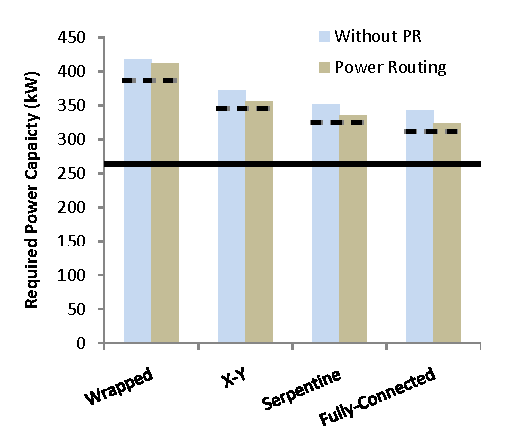
\includegraphics[width=3.0 in]{Appendices/PowerRouting/figure/result_AL.eps}
\label{figure::AL}
}
\hspace{0.5in}
\subfigure[MACC (high-performance computing)]{
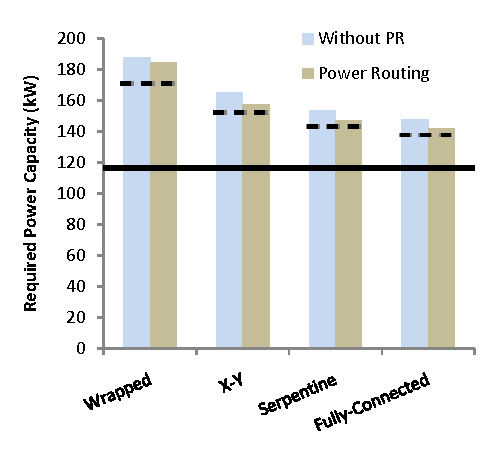
\includegraphics[width=3.0 in]{Appendices/PowerRouting/figure/result_nyx.eps}
\label{figure::nyx}
}
\vspace{-0.15 in}
\caption{ \textbf{\PowerRouting effectiveness in homogeneous data centers.} }
\vspace{-0.15 in}
\label{figure::homogenous}
\end{figure*}

To explore these effects, we construct \PowerRouting test cases for 1000-server synthetic clusters where each server runs the same application.  We do not study the web search application in isolation; in this application, the utilization on all servers rise and fall together, hence, the load on all PDUs is inherently balanced and there is no opportunity (nor need) for \PowerRouting. Instead, we evaluate \PowerRouting using the medical center traces and high performance computing traces, shown in Figures~\ref{figure::AL} and \ref{figure::nyx}, respectively. 

The high performance computing cluster consumes a time-average power of 114.9 kW, a maximum of 116.4 kW, and a standard deviation of 0.8 kW while the medical center computing traces consume a time-average power of 254.6 kW, with maximum 263.6 kW and standard deviation 2.4 kW.  In both cases, the variability is substantially lower than in the heterogeneous data center test case.

Although \PowerRouting comes close to achieving the theoretical lower bound infrastructure requirement in each case, we see that there is only limited room to improve upon the non-\PowerRouting case. Even the baseline wrapped topology requires infrastructure that exceeds the theoretical bound by only 7.5\% for the high performance computing cluster and 5\% for the medical data center. We conclude that \PowerRouting offers substantial improvement only in heterogeneous clusters and applications that see power imbalance, a common case in many facilities.

\subsection{\PowerRouting With Energy-Proportional Servers}
%{\bf \PowerRouting with Energy-Proportional Servers.}
As the gap between servers' peak and idle power demands grows  (e.g., with the advent of energy-proportional computers \cite{Barroso07}), we expect the potential for \PowerRouting to grow. The increase in power variance leads to a greater imbalance in power across PDUs, increasing the importance of correcting this imbalance with \PowerRouting.

To evaluate this future opportunity, we perform an experiment where we assume all servers are energy-proportional---that is, servers whose power draw varies linearly with utilization---with an idle power of just 10\% of peak.  This experiment models servers equipped with PowerNap \cite{Meisner09}, which allows servers to sleep during the millisecond-scale idle periods between task arrivals.  We repeat the experiment shown in Figure~\ref{figure::powerrouting} under this revised server power model. The results are shown in Figure~\ref{figure::powernap}.  Under these assumptions, our traces exhibit a time-average power of 99.8 kW, maximum of 153.9 kW, and standard deviation of 18.9 kW.

\PowerRouting is substantially more effective when applied to energy-proportional servers. 
However, the limitations of the wrapped topology are even more pronounced in this case, and \PowerRouting provides little improvement. Under the more-connected topologies, \PowerRouting is highly effective, yielding reductions of 22\%, 29\%, and 28\% for the X-Y, serpentine, and fully-connected topologies, respectively, relative to their counterparts without \PowerRouting.
As before, the more-connected topologies track their theoretical lower bounds more tightly.  Relative to the baseline wrapped topology, a serpentine topology with \PowerRouting yields a 47\% reduction in required physical infrastructure capacity. It is likely that as computers become more energy-proportional, power infrastructure utilization will continue to decline due to power imbalances.
\PowerRouting reclaims much of this wasted capacity.

\begin{figure}[t!]
\centering
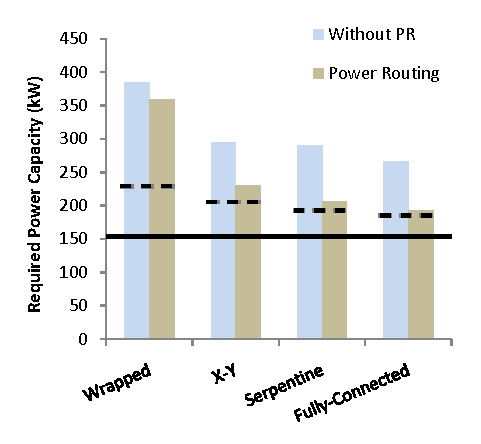
\includegraphics[width = 3.0 in]{Appendices/PowerRouting/figure/result_powernap.eps}
\vspace{-.1 in}
\caption{ \textbf{Impact with energy-proportional servers.} }
\label{figure::powernap}
\vspace{-.15 in}
\end{figure}


\subsection{Limitations}

Our evaluation considers workloads in which any server may be throttled, and our mechanisms make no effort to select servers for throttling based on any factors except maximizing the utilization of the power delivery infrastructure.  In some data centers, it may be unacceptable to throttle performance.  These data centers cannot gain a capital cost savings from under-provisioning; their power infrastructure must be provisioned for worst case load.  Nonetheless, these facilities can benefit from intermixed topologies (to reduce reserve capacity for fault tolerance) and from the phase-balancing possible with \PowerRouting.
 

% Conclusion
\section{Conclusion}
\label{section::conclusion}

The capital cost of power delivery infrastructure is one of the largest components of data center cost, rivaling energy costs over the life of the facility.  In many data centers, expansion is limited because available power capacity is exhausted.  To extract the most value out of their infrastructure, data center operators over-subscribe the power delivery system.  As long as individual servers connected to the same PDU do not reach peak utilization simultaneously, over-subscribing is effective in improving power infrastructure utilization.  However, coordinated utilization spikes do occur, particularly among collocated machines, which can lead to substantial throttling even when the data center as a whole has spare capacity.

In this paper, we introduced a pair of complementary mechanisms, shuffled power distribution topologies and \PowerRouting, that reduce performance throttling and allow cheaper capital infrastructure to achieve the same performance levels as current data center designs.  Shuffled topologies permute power feeds to create strongly-connected topologies that reduce reserve capacity requirements by spreading responsibility for fault tolerance.  \PowerRouting schedules loads across redundant power delivery paths to shift power delivery slack to satisfy localized utilization spikes.  Together, these mechanisms reduce capital costs by 32\% relative to a baseline high-availability design when provisioning for zero performance throttling. Furthermore, with energy-proportional servers, the power capacity reduction increases to 47\%.


% Acknowledgements
%\section{Acknowledgements}
This work was partially supported by grants and equipment from Intel and Mentor Graphics and NSF Grant CCF-0811320.



%%%\begin{spacing}{1.0}
%%%\bibliographystyle{IEEEtranS}
%%%\bibliography{abbrev,PowerRouting}
%%%\end{spacing}
%%%
%%%
%%%\end{document}

 %\appendix{Two-Dimensional Crank-Nicolson Scheme for a Uniform Spherical Grid}
 %\label{app:CN Scheme}
 %\input{Appendices/Appendix_Open_Flux}
 
\startbibliography
 \begin{singlespace} % Bibliography must be single spaced
  \bibliography{References}   % Use the BibTeX file ``References.bib''.
 \end{singlespace}

% An external Abstract that can be printed at the end of the document, 
% for separate submission to Rackham. Comment it out when not needed. - jg
%\startextabstractpage
%{The Title of Your Dissertation}{Your Name}{Chair: Albert Einstein}
%Emerging storage technologies offer an alternative to disk that is durable and allows faster data access.
Flash memory, made popular by mobile devices, provides block access with low latency random reads.
Additionally, new nonvolatile memories (NVRAM) are expected in upcoming years, presenting DRAM-like performance alongside persistent storage.
Wheres both technologies accelerate data access due to their raw speed, used merely as a disk replacement they may fail to achieve their full potentials.
Flash's asymmetric read/write access (i.e., reads execute faster than writes) opens new opportunities to optimize Flash-specific access.
Similarly, NVRAM's low latency persistent accesses allow new designs for high performance failure-resistant applications.

This thesis addresses software and hardware system design for such storage technologies.
First, I investigate analytics query optimization for Flash, expecting Flash's fast random access to require new query planning.
While Flash allows some queries to benefit from alternative query optimization, the range of queries affected and relative performance increase is negligible.
Second, I examine new opportunities for durable, recoverable transaction processing with NVRAM.
Existing disk-based recovery mechanisms impose large software overheads, yet updating data in-place requires frequent device synchronization that limits throughput.
Subsequently, I introduce a new design, \GroupCommit, to amortize synchronization delays over many transactions, increasing throughput at some cost to transaction latency.
Finally, I propose to research programming interfaces and hardware designs to enable intuitive, high performance recoverable data structures with NVRAM, extending memory consistency with persistent semantics to introduce \emph{Persistent Memory Consistency}.

%\label{ExtAbstract}

\end{document}
